\documentclass[a4paper]{report}
\usepackage{header}
\usepackage[
    top=1in,
    bottom=1in,
    left=1in,
    right=1in
]{geometry}

\begin{document}
\begin{titlepage}
\begin{center}
VIETNAM NATIONAL UNIVERSITY, HO CHI MINH CITY \\
UNIVERSITY OF TECHNOLOGY \\
FACULTY OF COMPUTER SCIENCE AND ENGINEERING
\end{center}

\vspace{3cm}

\begin{figure}[h!]
\begin{center}

\includegraphics[width=3cm]{hcmut.png}
\end{center}
\end{figure}

\vspace{1cm}


\begin{center}
\begin{tabular}{c}
\multicolumn{1}{l}{\textbf{{\Large SOFTWARE ENGINEERING (CO3001)}}}\\
~~\\
\hline
\\
\multicolumn{1}{l}{\textbf{{\Large Assignment}}}\\
\\
\textbf{{\Huge Student Smart Printing Service}}\\
\\
\hline
\end{tabular}
\end{center}

\vspace{3cm}

\begin{table}[h]
\begin{tabular}{rrl}
\hspace{5 cm} & Advisor: & Truong Tuan Anh\\

& Students: & Do Thanh Trung – 2252853\\
& & Do Quang Khanh – 2053106 \\
& & Ha The Binh – 2152435\\
& & Ho Minh Hoang – 2211073 \\
& & Hoang Huy Minh – 2053212
\end{tabular}
\end{table}


    \vspace*{5cm} % Pushes content to the bottom of the page
    \begin{center}
        {\footnotesize HO CHI MINH CITY, OCTOBER 2024}
    \end{center}
\end{titlepage}


%\thispagestyle{empty}

\newpage
\tableofcontents
\newpage


%%%%%%%%%%%%%%%%%%%%%%%%%%%%%%%%%
\vspace{5cm}

\begin{table}[H]
\renewcommand{\arraystretch}{1.8}
\centering
\begin{tabular}{|c|p{3cm}|c|p{6cm}|c|}
\hline
\textbf{No.} & \textbf{Fullname} & \textbf{Student ID} & \textbf{Tasks} & \textbf{Completion} \\
\hline
1 & Do Quang Khanh   & 2053106   & -                     & 100\% \\
\hline
2 & Ho Minh Hoang    & 2211073   & - Integration \& Report \newline
- Table format for usecase diagram& 100\% \\
\hline
3 & Do Thanh Trung   & 2252853   & - Domain Context \newline - F \& NF requirements \newline - Usecase diagram     & 100\% \\
\hline
4 & Ha The Binh      & 2152435   & - Domain Context \newline - F \& NF requirements & 100\% \\
\hline
5 & Hoang Huy Minh   & 2053212   & -               & 100\% \\
\hline
\end{tabular}
\caption{Table of Workload Distribution for Task 1}
\end{table}

\begin{table}[H]
\renewcommand{\arraystretch}{1.8}
\centering
\begin{tabular}{|c|p{3cm}|c|p{6cm}|c|}
\hline
\textbf{No.} & \textbf{Fullname} & \textbf{Student ID} & \textbf{Tasks} & \textbf{Completion} \\
\hline
1 & Do Quang Khanh & 2053106 & - Activity Diagram & 100\% \\
\hline
2 & Ho Minh Hoang & 2211073 & - Sequence Diagram & 100\% \\
\hline
3 & Do Thanh Trung & 2252853 & - Class Diagram & 100\% \\
\hline
4 & Ha The Binh      & 2152435   & - Development MVP 1 & 100\% \\
\hline
5 & Hoang Huy Minh   & 2053212   & - Report               & 100\% \\
\hline
\end{tabular}
\caption{Table of Workload Distribution for Task 2}
\end{table}

\begin{table}[H]
\renewcommand{\arraystretch}{1.8}
\centering
\begin{tabular}{|c|p{3cm}|c|p{6cm}|c|}
\hline
\textbf{No.} & \textbf{Fullname} & \textbf{Student ID} & \textbf{Tasks} & \textbf{Completion} \\
\hline
1 & Do Quang Khanh & 2053106 & - & 100\% \\
\hline
2 & Ho Minh Hoang & 2211073 & - Architecture Diagram & 100\% \\
\hline
3 & Do Thanh Trung & 2252853 & - Integration \& Report \newline - Redesign UI with Figma & 100\% \\
\hline
4 & Ha The Binh      & 2152435   & - Component Diagram & 100\% \\
\hline
5 & Hoang Huy Minh   & 2053212   & -& 100\% \\
\hline
\end{tabular}
\caption{Table of Workload Distribution for Task 3}
\end{table}



\newpage


\chapter{Requirement Elicitation}

\section{Domain Context}
With the increasing demand for accessible and efficient printing services among students on campus, the HCMUT Smart Printing Service (HCMUT$\_$SSPS) is designed to address these needs by offering a centralized and user-friendly printing solution. Traditionally, students had to leave the campus to reach printing shops, which can be both time-consuming and inconvenient, especially when tight schedules or emergency arises. On top of that, external services may not offer the flexibility when it comes to printing options. Therefore, HCMUT$\_$SSPS aims to tackle these problems by offering a seamless on-campus printing service where students can easily upload documents, configure print settings, and pick up their paperwork from nearby printers without leaving the university.

The HCMUT$\_$SSPS system is designed to address these issues by offering an all-in-one printing solution directly on campus, allowing students to upload documents, choose from a variety of print options, and select their nearest campus printer through a web-based or mobile interface. This further facilitate students to fully customize their print jobs according to their preferences. In other words, the service allows for a seamless printing experience without the hassle of third-party shops. Moreover, with multiple printers located across different campus buildings, students can easily find a printer near them. With this option, students can plan around their busy academic timetable.

Beyond convenience, the system enhances security by keeping sensitive information locally since students no longer need to share personal information with external printing services, the risk of data breaches is reduced. The authentication functionality also allows students to track their printing history, providing transparency and an easy way to track usage. This combination of convenience, highly customization and keeping confidential data locally makes HCMUT$\_$SSPS an invaluable resource for students, streamlining the printing process and integrating it into campus life

\section{Stakeholders and Needs}
\vspace{-0.2em}
\begin{enumerate}[label=\textbf{\arabic*}.]
    \item \textbf{Students}
    users of the printing services. They can send print request, upload docu ments and purchase additional papers.  Students need the service to be easy to use, accessible from all places and secured along with the ability to review printing history.  
    \item \textbf{Student Printing Service Officer (SPSO)}
    who is responsible for managing student printing activities. The SPSO needs to manage printer settings, track and log printing activities and useful management tools.
    \item \textbf{IT staff}
    who responsible for developing, maintaining and upgrading the system. They need to build and develop the service for the university. 
    \item \textbf{University Administators}
    who manages resources and online payments system like BKPay. They need to be able to allocate resources and monitor transaction effectively. 
\end{enumerate}

\section{Benefits of the System}

\begin{itemize}
    \item \textbf{Students}
    
    Because of the user-friendly interface and accessible service like a web page, students can save time, increasing their productivity and satisfactory. Students also can format the documents to match their requirements. 
    \item \textbf{SPSO}
    
    The SPSO will be able to manage printing resources and settings efficiently. They can also review detailed reports of students’ printing activities, leading to better operational insights.
    \item \textbf{IT staff}
    
    The IT department can enhance users’ satisfactory and generate economic benefits for the service providers.
    \item \textbf{University Administrators}
    
    They can get a higher reputation and better financial efficiency through streamlined payments. 
\end{itemize}

\section{Functional Requirements}
\textbf{For Students}
\begin{enumerate}
    \item Students have the ability to upload documents for printing.
    \item Students can select printers and printing options, such as page size, number of copies, etc.
    \item They can view their printing history and page balances.
    \item Ability to purchase additional pages through an online payment system.
    \item Students can observe the status of print jobs, including start and end times, so they can determine when their prints are ready.
\end{enumerate}
\textbf{For SPSO}
\begin{enumerate}
    \item Ability to add, enable, or disable printers.
    \item SPSO can configure system settings such as page quotas and file types.
    \item SPSO can track the printing logs of students.
    \item SPSO has access to monthly and annual reports and can view them at any time.
    \item SPSO can schedule default page quotas for students each semester.
\end{enumerate}
\textbf{For IT staff}
\begin{enumerate}
    \item IT staff must be able to monitor the system’s performance, including server status, network connectivity, and printer availability across campus in real-time.
    \item IT staff must be able to add, remove, or troubleshoot printers within the network to ensure they are correctly connected to the system and operating properly.
    \item IT staff can maintain the HCMUT\_SSO authentication system, ensuring that students and staff can securely log in to the system.
    \item IT staff can create backups of the system's data (e.g., printing logs, configurations, user data) and perform data recovery in case of a failure.
    \item IT staff should be able to access and review system logs to troubleshoot any issues (e.g., failed print jobs, server errors, user access problems) and take corrective actions when necessary.
\end{enumerate}
\newpage
\textbf{For University Administrators}
\begin{enumerate}
    \item They can view system usage reports, such as the number of pages used, student printing activities, or dates.
    \item They must be able to monitor financial transactions through BKPay services.
    \item They can configure the default number of pages allocated to each student.
    \item They also have access to printing logs and resource usage.
    \item They can define roles and permissions for users, such as students, SPSO, and IT staff, so that each person can perform certain actions.
\end{enumerate}

\section{Non-Functional Requirements}
\begin{enumerate}
    \item The system should be accessible on both web and mobile platforms.
    \item The system must ensure user authentication via HCMUT\_SSO and enable payments via BKPay services.
    \item The system should facilitate fast and efficient document upload and printing.
    \item The system should handle large numbers of students and printers efficiently, supporting up to 1000 concurrent requests.
    \item To protect users' privacy, the system must ensure data confidentiality for printing logs and payment details.
\end{enumerate}

\section{Use-case Diagrams}
\subsection{Use-case Diagram for the Whole System}
\begin{figure}[H]
    % \vspace{-0.5cm}
    \centering
    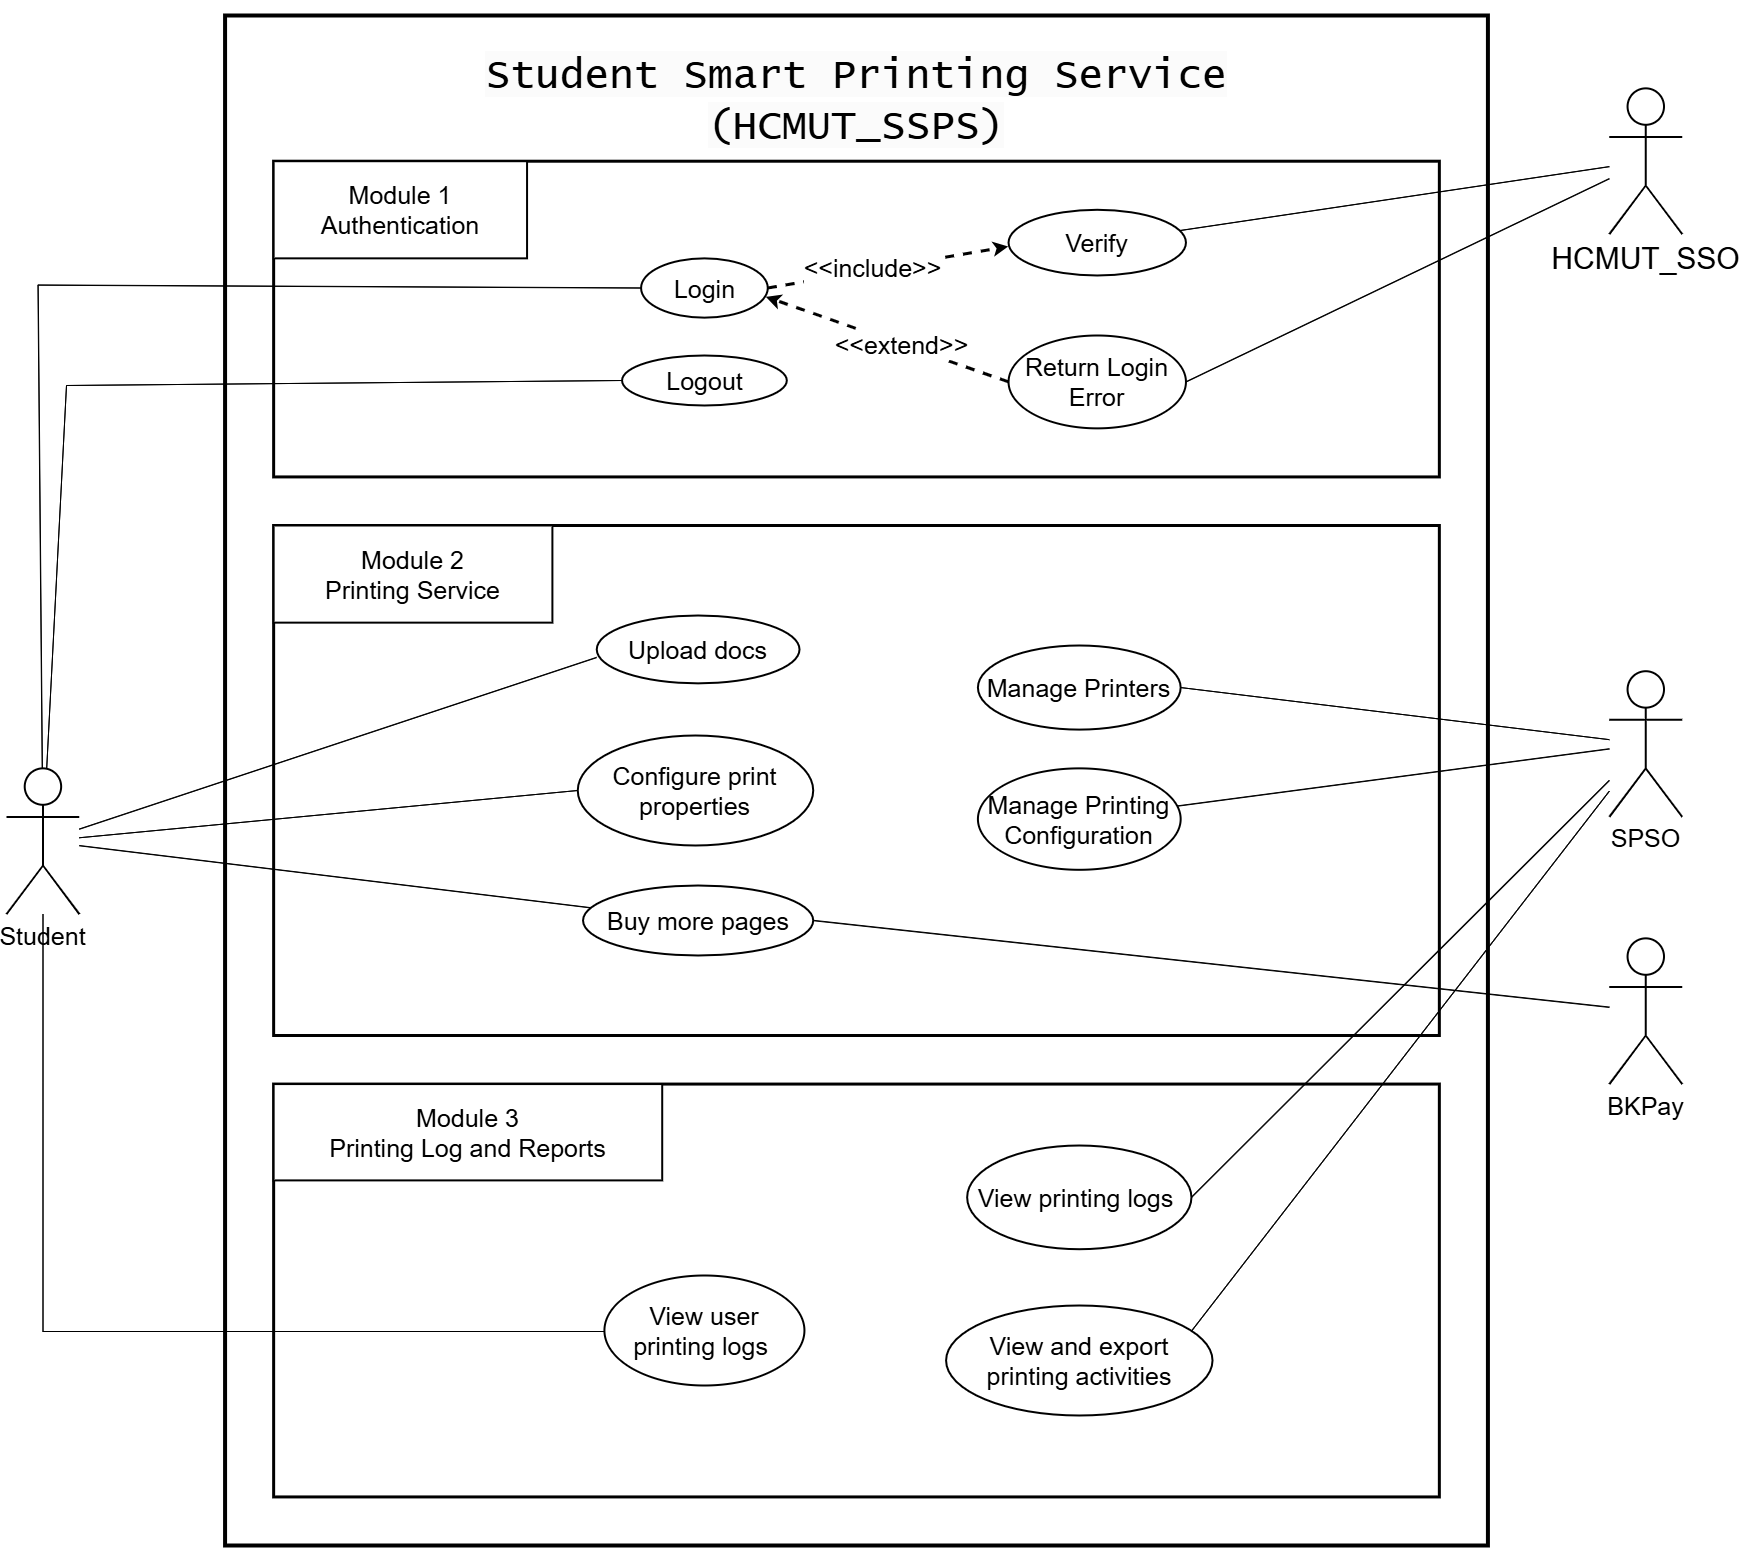
\includegraphics[width=\textwidth]{images/usecase_diagram/use_case_whole_system.png}
    \caption{Use-case Diagram for Whole System}
    \label{fig:use_case_whole_system}
\end{figure}

\clearpage
\begin{table}[h!]
\centering
\renewcommand{\arraystretch}{1.8}
% \small % Reduce font size for the table
\begin{tabular}{|>{\raggedright\arraybackslash}p{3cm}|>{\centering\arraybackslash}p{3cm}|p{7cm}|}
\hline
\textbf{Use Case Name} & \textbf{Actors} & \textbf{Description} \\ \hline
Login & Student,  HCMUT\_SSO & Allows the student to log in using HCMUT\_SSO authentication. \\ \hline
Logout & Student & Logs out the student from the system. \\ \hline
Upload Document & Student & Students upload documents to be printed by selecting a printer and configuring print properties. \\ \hline
Configure Print Properties & Student & Allows students to specify details like paper size, page range, and number of copies for printing. \\ \hline
Buy More Pages & Student, BKPay & Students purchase additional pages for printing by making a payment through BKPay. \\ \hline
View Printing Logs & Student, SPSO & Students and SPSO can view printing logs filtered by time period and printer. \\ \hline
Manage Printers & SPSO & SPSO can add, enable, or disable printers and modify printer configurations. \\ \hline
Manage Printing Configuration & SPSO & SPSO can manage settings like permitted file types and default page allocations. \\ \hline
View and Export Printing Activities & SPSO & SPSO can generate reports and export data on the usage of the printing service. \\ \hline
Authenticate Users & HCMUT\_SSO & HCMUT\_SSO authenticates students and SPSO before they can access the system. \\ \hline
Manage Page Quota & SPSO & SPSO can set default page quotas for students and update them during the semester. \\ \hline
Payment Processing & BKPay & Handles payment transactions for students purchasing more pages. \\ [2ex] \hline
\end{tabular}
\caption{Use-case Table for Whole System}
\label{tab:use_case_table_whole_system}
\end{table}




\subsection{Use-case Diagram for Printing Service Module}

\begin{figure}[H]
    % \vspace{-0.5cm}
    \centering
    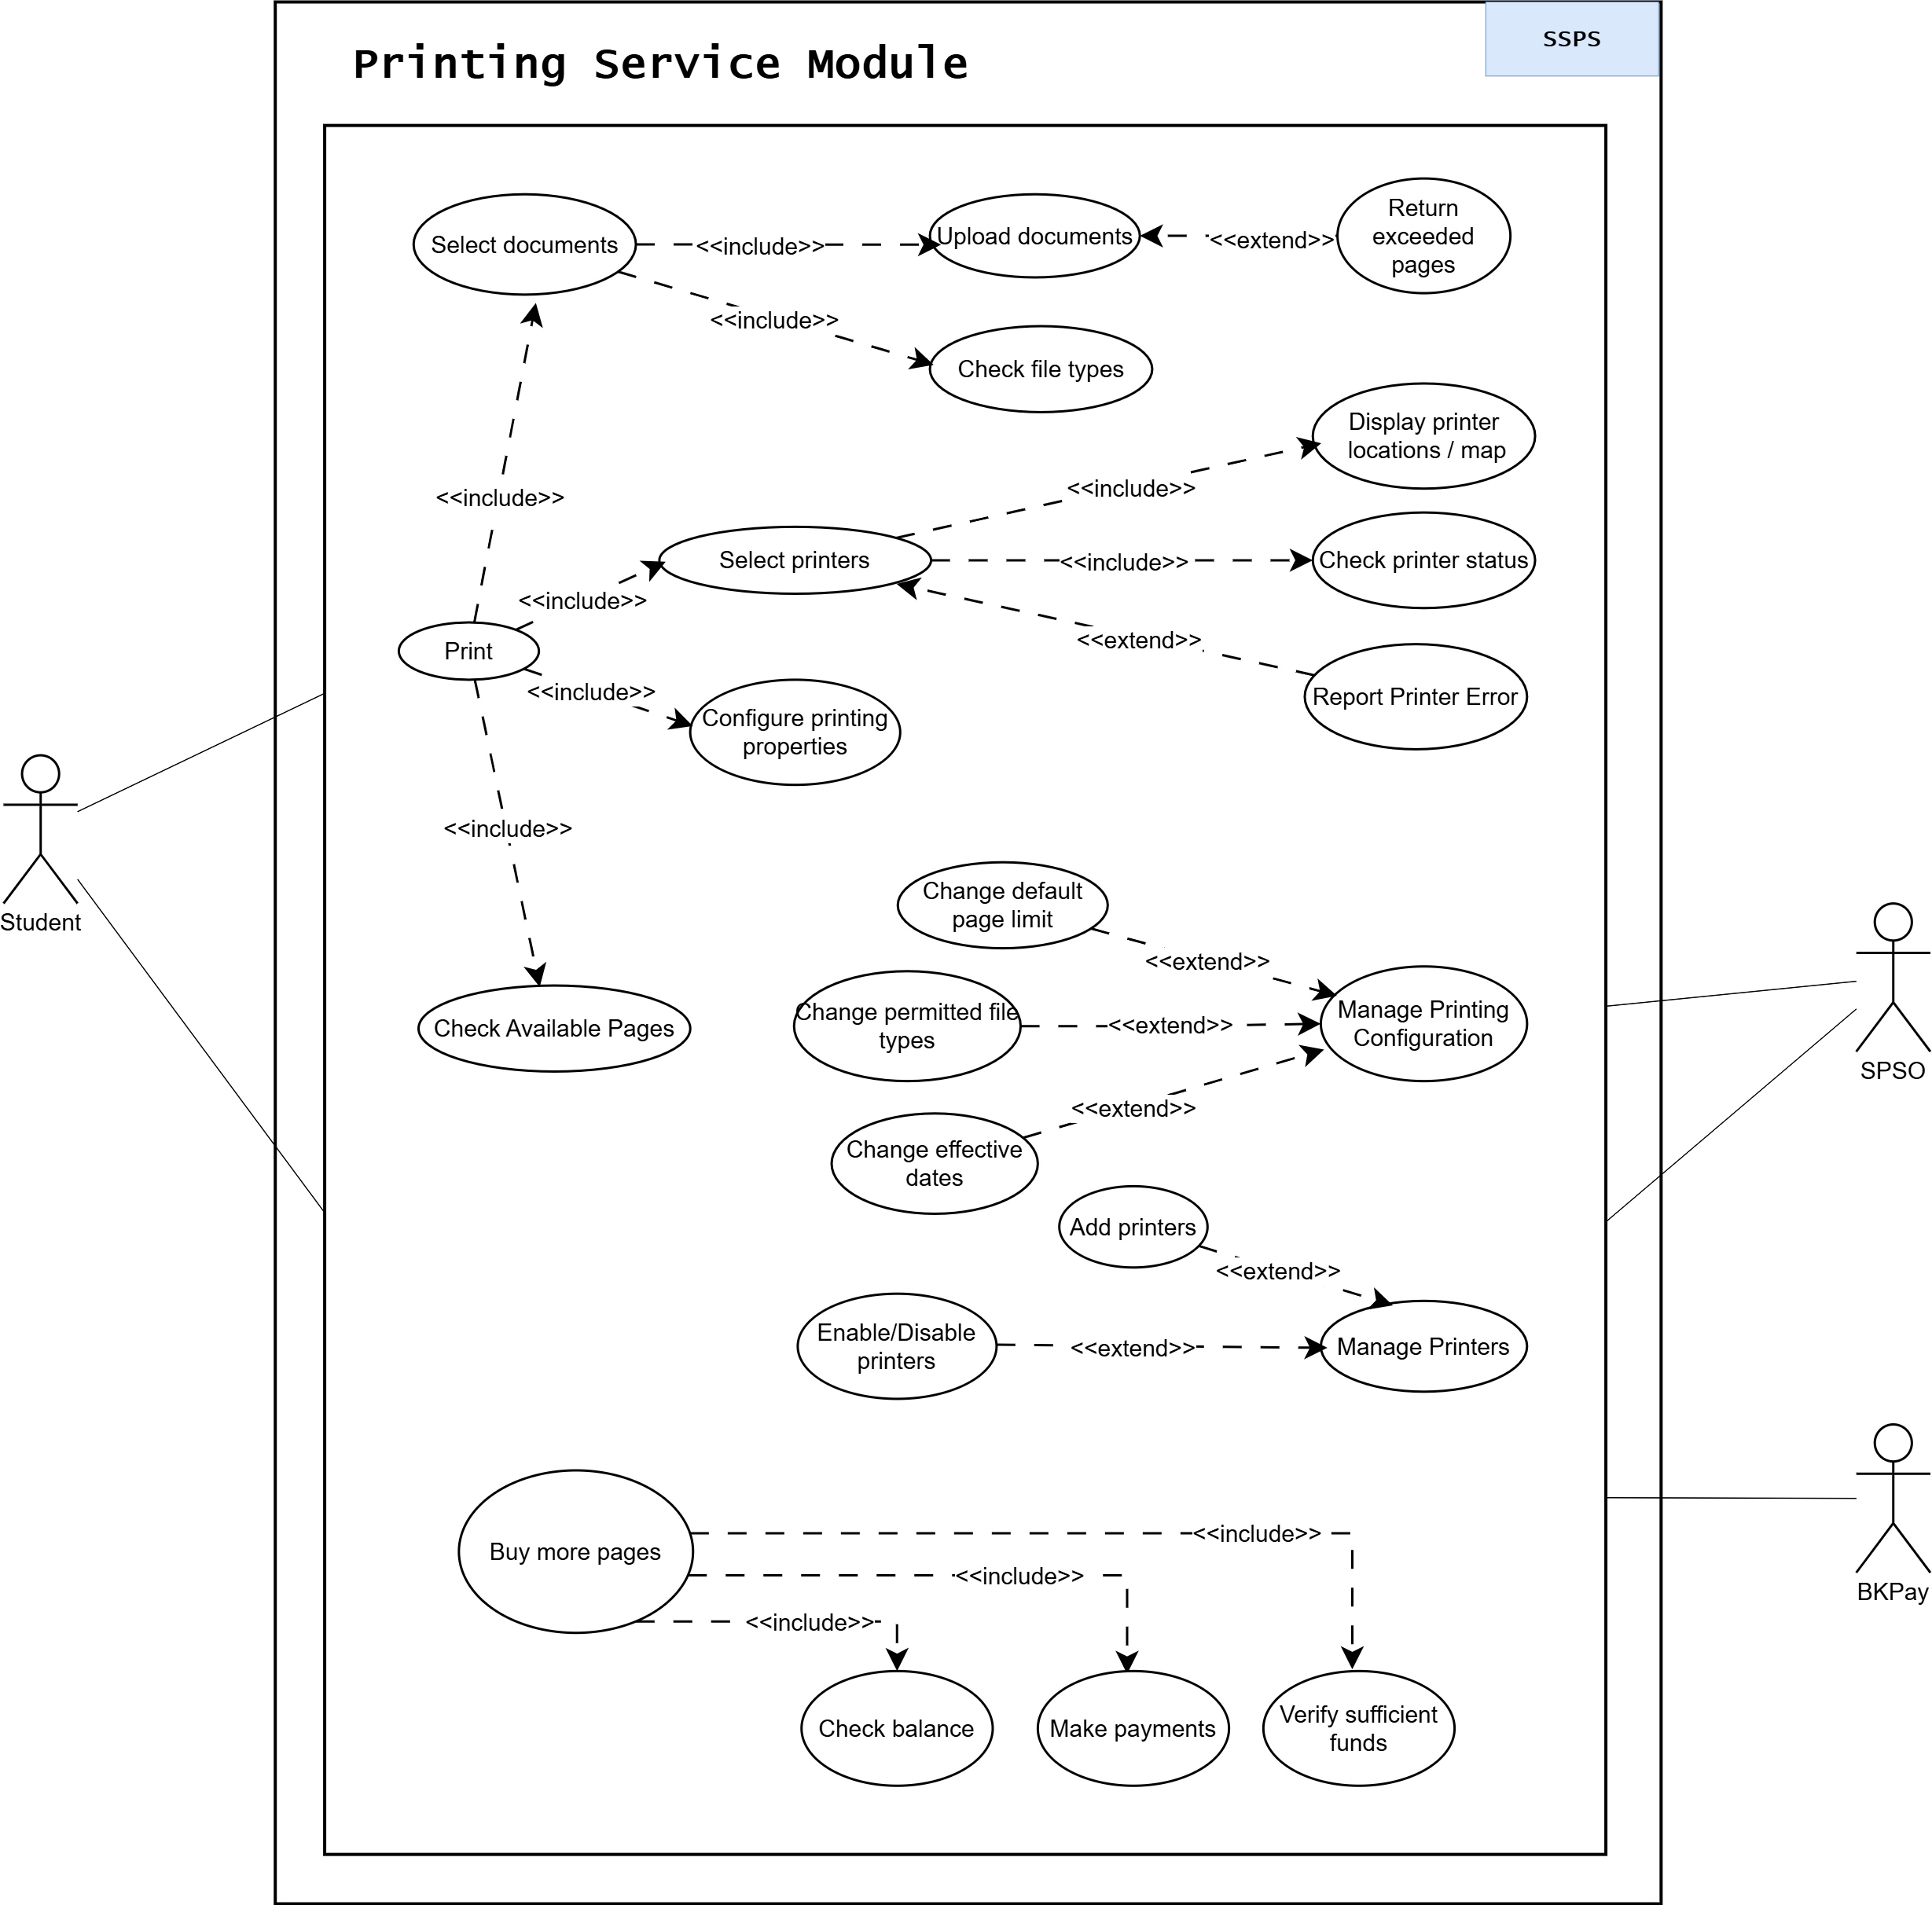
\includegraphics[width=\textwidth]{images/usecase_diagram/use_case_printing_service.png}
    \caption{Use-case Diagram for Printing Service Module}
    \label{fig:use_case_printing_service}
\end{figure}

\clearpage
\begin{table}[h!]
\centering
\renewcommand{\arraystretch}{1.8}
% \small % Reduce font size for the table
\begin{tabular}{|>{\raggedright\arraybackslash}p{3cm}|>{\centering\arraybackslash}p{3cm}|p{7cm}|}
\hline
\textbf{Use Case Name} & \textbf{Actors} & \textbf{Description} \\ \hline
Upload Documents & Student & The student uploads a document to be printed, and the system checks for supported file types. \\ \hline
Select Printer & Student & Allows the student to select a printer from a list or map based on availability. \\ \hline
Configure Printing Properties & Student & The student can configure the print job settings such as paper size, double-sided printing, and number of copies. \\ \hline
Print Documents & Student, Printer & The student sends the print job to the selected printer after configuring print settings. \\ \hline
Check Available Pages & Student & The system shows the student how many pages they can print based on their current balance. \\ \hline
Buy More Pages & Student, BKPay & The student buys additional printing pages by making a payment through BKPay. \\ \hline
Manage Printers & SPSO & The SPSO can add, enable, or disable printers, and check their statuses. \\ \hline
Manage Printing Configuration & SPSO & SPSO can change printing configurations such as default page limits, permitted file types, and effective dates. \\ \hline
Check Balance & Student, BKPay & Checks the student’s BKPay balance before making a payment for additional pages. \\ \hline
Make Payments & Student, BKPay & The student makes a payment for additional pages through BKPay. \\ \hline
Verify Sufficient Funds & BKPay & BKPay verifies that the student has sufficient funds to complete the payment for additional printing pages. \\ \hline
Return Exceeded Pages & System & If a student prints more pages than their balance allows, the system adjusts and refunds the exceeded portion. \\ \hline
Report Printer Error & Printer, System & If a printer encounters a technical problem (e.g., paper jam, out of ink), it reports the issue to the SPSO and the student. \\ [1ex] \hline
\end{tabular}
\caption{Use-case Table for Printing Service Module}
\label{tab:printing_service_use_case}
\end{table}

\newpage
\subsection{The Details of Usecases in Printing Service Module}

\begin{enumerate}\bfseries
    \item Usecase Login
    
       \begin{table}[h!]
        \centering
        \renewcommand{\arraystretch}{1.8}
        \begin{tabular}{|>{\centering\arraybackslash}m{3cm}|>{\raggedright\arraybackslash}m{10cm}|}
        \hline
        \textbf{Use Case Name} & Login \\ \hline
        \textbf{Actor(s)} & Student, HCMUT\_SSO \\ \hline
        \textbf{Description} & This use case describes the process by which a student logs into the system using their credentials. The student enters their username and password, and the system verifies these credentials via the HCMUT\_SSO service. Upon successful authentication, the student is granted access to the system’s features, such as uploading documents, viewing logs, and managing their printing account. \\ \hline
        \textbf{Preconditions} & The student must have valid login credentials. \\ \hline [2ex]
        \textbf{Basic Flow} &
        \begin{enumerate}
            \item The student selects the "Login" option.
            \item The system requests authentication details (username, password).
            \item The student enters their credentials.
            \item The system sends the credentials to HCMUT\_SSO for verification.
            \item HCMUT\_SSO verifies the credentials.
            \item The system logs the student in and grants access to printing services.
        \end{enumerate} \\ \hline
        \textbf{Alternative Flows} & If the credentials are incorrect, HCMUT\_SSO returns an error, and the system displays a "Login Error" message to the student. \\ \hline
        \textbf{Postconditions} & The student is logged in and can access the system’s services. \\ \hline
        \textbf{Exceptions} & If the HCMUT\_SSO service is unavailable, the system displays an error message and prompts the student to retry later. \\ [2ex] \hline
        \end{tabular}
        \caption{Use-case Table for Use Case “Login”}
        \label{tab:login_use_case}
        \end{table}
    \newpage
    \item Usecase Upload Documents
    

    
        \begin{table}[h!]
            \centering
            \renewcommand{\arraystretch}{1.8}
            \begin{tabular}{|>{\centering\arraybackslash}m{3cm}|>{\raggedright\arraybackslash}m{10cm}|}
            \hline
            \textbf{Use Case Name} & Upload Document \\ \hline
            \textbf{Actor(s)} & Student \\ \hline
            \textbf{Description} & The student uploads a document, selects a printer, and configures print settings. The system verifies the file type and processes the document for printing. \\ \hline
            \textbf{Preconditions} & The student must be logged in. The printer must be available. \\ \hline
            \textbf{Basic Flow} & 
            \begin{enumerate}
                \item The student selects the "Upload Documents" option.
                \item The system presents a file upload interface.
                \item The student uploads a document.
                \item The system verifies the file format (supported file types only).
                \item The student selects the printer and configures print properties.
                \item The system processes the document and sends it to the printer.
            \end{enumerate} \\ [-2ex] \hline
            \textbf{Alternative Flows} & If the file format is not supported, the system displays an error message and prompts the student to upload a valid file. \\ \hline
            \textbf{Postconditions} & The document is uploaded and queued for printing. \\ \hline
            \textbf{Exceptions} & 
            \begin{enumerate}
                \item \textbf{Unsupported File Format:} The system checks the document's file type and finds it unsupported (e.g., not PDF, DOCX). The system displays an error message: "Unsupported file format. Please upload a document in a supported format (PDF, DOCX, etc.)." The student is prompted to upload a valid file type.
                \item \textbf{File Size Too Large:} The system checks the file size and finds it exceeds the allowed limit. The system displays an error message: "File size too large. Please upload a file smaller than X MB." The student is prompted to upload a smaller file.
                \item \textbf{Network Issues:} The system detects network problems during the file upload. It displays an error message: "Network error. Please check your connection and try again." The system prompts the student to retry once the connection is restored.
            \end{enumerate} \\ \hline
            \end{tabular}
            \caption{Use-case Table for Use Case “Upload Document”}
            \label{tab:upload_document_use_case}
        \end{table}

    \newpage
    \item Usecase Buy More Pages
    
        \begin{table}[h!]
            \centering
            \renewcommand{\arraystretch}{1.8}
            \begin{tabular}{|>{\centering\arraybackslash}m{3cm}|>{\raggedright\arraybackslash}m{10cm}|}
            \hline
            \textbf{Use Case Name} & Buy More Pages \\ \hline
            \textbf{Actor(s)} & Student, BKPay \\ \hline
            \textbf{Description} & The student purchases additional printing pages through BKPay, and the system updates their account. \\ \hline
            \textbf{Preconditions} & The student must be logged in. The printer must be available. \\ \hline
            \textbf{Basic Flow} & 
            \begin{enumerate}
                \item The student selects "Buy More Pages".
                \item The system shows available packages.
                \item The student selects a package.
                \item The system redirects to BKPay for payment.
                \item The student completes the payment.
                \item BKPay confirms the transaction, and the system credits the student's account.
            \end{enumerate} \\ \hline
            \textbf{Alternative Flows} & 
            If the payment fails:
            \begin{enumerate}
                \item The system notifies the student that the payment was unsuccessful.
                \item The system presents options to retry the payment or select a different payment method. The student can:
                \begin{itemize}
                    \item Retry the transaction with the same payment method.
                    \item Select a different payment method from their BKPay account (e.g., different credit card or bank account).
                \end{itemize}
                \item The student attempts the transaction again, either by retrying the original method or using the alternative method.
                \item If successful, BKPay confirms the payment, and the system credits the student's account with the additional pages.
                \item If the payment fails again, the student is prompted to contact support or try later.
            \end{enumerate} \\ \hline
            \textbf{Postconditions} & The student's account is updated with the additional pages. \\ \hline
            \textbf{Exceptions} & If BKPay is unavailable, the system displays an error and advises the student to try again later. \\ [2ex] \hline
            \end{tabular}
            \caption{Use-case Table for Use Case “Buy More Pages”}
            \label{tab:buy_more_pages_use_case}
        \end{table}

    \newpage
    \item Usecase Manage Printers
    
        \begin{table}[h!]
            \centering
            \renewcommand{\arraystretch}{1.8}
            \begin{tabular}{|>{\centering\arraybackslash}m{3cm}|>{\raggedright\arraybackslash}m{10cm}|}
            \hline
            \textbf{Use Case Name} & Manage Printers \\ \hline
            \textbf{Actor(s)} & SPSO (Student Printing Service Officer) \\ \hline
            \textbf{Description} & This use case allows the SPSO to manage the printers in the system. The SPSO can add new printers, enable or disable existing printers, and modify printer details. The system saves these changes and updates the printer configurations for use by students. \\ \hline
            \textbf{Preconditions} & The SPSO must be logged in with administrative privileges. \\ \hline
            \textbf{Basic Flow} & 
            \begin{enumerate}
                \item The SPSO selects the "Manage Printers" option.
                \item The system displays a list of available printers.
                \item The SPSO can add new printers, enable or disable existing printers, or edit printer details.
                \item The SPSO submits the changes.
                \item The system saves the changes and updates the printer configurations.
            \end{enumerate} \\ \hline
            \textbf{Alternative Flows} & 
            If the printer cannot be added due to incorrect details (e.g., invalid location or model number):
            \begin{enumerate}
                \item The system detects the error in the printer details and prevents the submission.
                \item The system displays an error message describing the problem (e.g., "Invalid model number or location").
                \item The SPSO is prompted to correct the printer details.
                \item The SPSO corrects the input and resubmits.
                \item The system verifies the new input and, if valid, saves the changes successfully.
            \end{enumerate} \\ \hline
            \textbf{Postconditions} & The printer configurations are updated in the system and are available for student use. \\ \hline
            \textbf{Exceptions} & If the system fails to update the printer list due to technical issues, the SPSO is notified to try again later. \\ [2ex] \hline
            \end{tabular}
            \caption{Use-case Table for Use Case “Manage Printers”}
            \label{tab:manage_printers_use_case}
        \end{table}

    \newpage
    \item Usecase View Printing Logs
        \begin{table}[h!]
            \centering
            \renewcommand{\arraystretch}{1.8}
            \begin{tabular}{|>{\centering\arraybackslash}m{3cm}|>{\raggedright\arraybackslash}m{10cm}|}
            \hline
            \textbf{Use Case Name} & View Printing Logs \\ \hline
            \textbf{Actor(s)} & Student, SPSO \\ \hline
            \textbf{Description} & This use case allows the user (either a student or SPSO) to view the printing logs. The user can filter logs by date range and printer, and the system provides a summary of the number of pages printed by paper size. \\ \hline
            \textbf{Preconditions} & The user (student or SPSO) must be logged in to the system. \\ \hline
            \textbf{Basic Flow} & 
            \begin{enumerate}
                \item The user selects the "View Printing Logs" option.
                \item The system displays a list of logs for the selected time.
                \item The user can filter the logs by date range and printer.
                \item The system provides a summary of the printed pages by size (e.g., A4, A3).
            \end{enumerate} \\ \hline
            \textbf{Alternative Flows} & 
            If no logs are found for the selected period:
            \begin{enumerate}
                \item The system checks if there are any printing logs for the chosen time period and printer.
                \item If no logs are available, the system displays a message: "No logs found for the selected time period."
                \item The user can adjust the filters or select a different time period or printer.
            \end{enumerate} \\ \hline
            \textbf{Postconditions} & The requested printing logs are displayed to the user, including a summary of the number of pages printed by size. \\ \hline
            \textbf{Exceptions} & If the system fails to retrieve the logs:
            \begin{enumerate}
                \item The system encounters a problem while trying to access the logs (e.g., database connection error).
                \item The system displays an error message: "Unable to retrieve logs at this time. Please try again later."
                \item The user is prevented from viewing logs until the issue is resolved.
            \end{enumerate} \\ \hline
            \end{tabular}
            \caption{Use-case Table for Use Case “View Printing Logs”}
            \label{tab:view_printing_logs_use_case}
        \end{table}
\end{enumerate}


\chapter{System Modeling}
\section{Activity Diagram}

\begin{figure}[H]
    \centering
    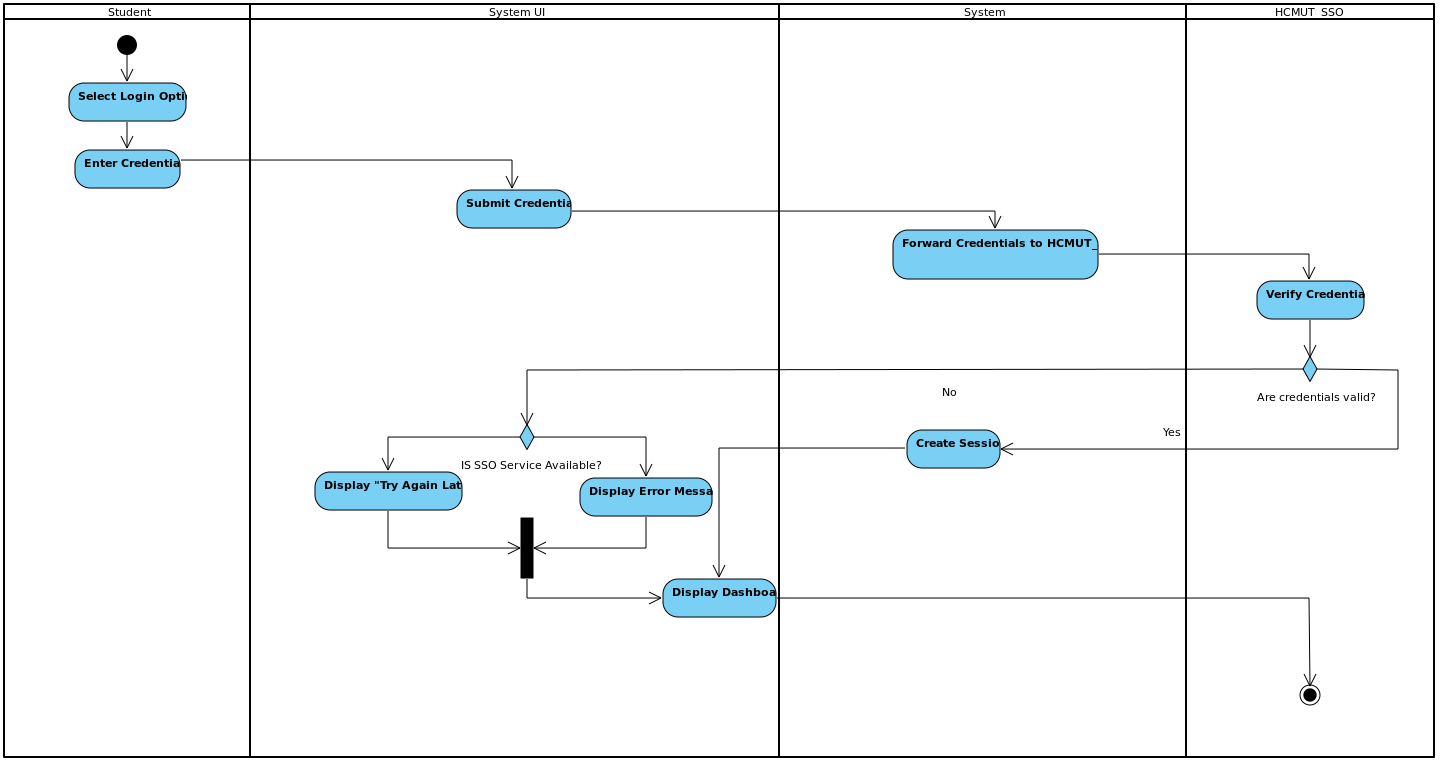
\includegraphics[width = 5in]{activity_diagram/login.png}
    \caption{UseCase - Login}
\end{figure}

This diagram illustrates the login process for a student accessing the HCMUT Student Smart Printing Service (HCMUT\_SSPS) through the HCMUT Single Sign-On (SSO) authentication service.

The process begins when a Student selects the login option and enters their credentials. These credentials are then submitted through the System UI, which forwards them to the System and subsequently to the HCMUT SSO service.

In the HCMUT SSO lane, the credentials are verified. If the credentials are invalid, the process will terminate with an error message displayed back to the user. If the credentials are valid, the System creates a session for the user, enabling successful login. If there are issues connecting to the SSO service, an error or "try again later" message is displayed to the student. If successful, the Dashboard is displayed to the user, concluding the login process.

This diagram covers key decision points, such as credential validity checks and service availability, to handle different scenarios in the login workflow.

\begin{figure}[H]
    \centering
    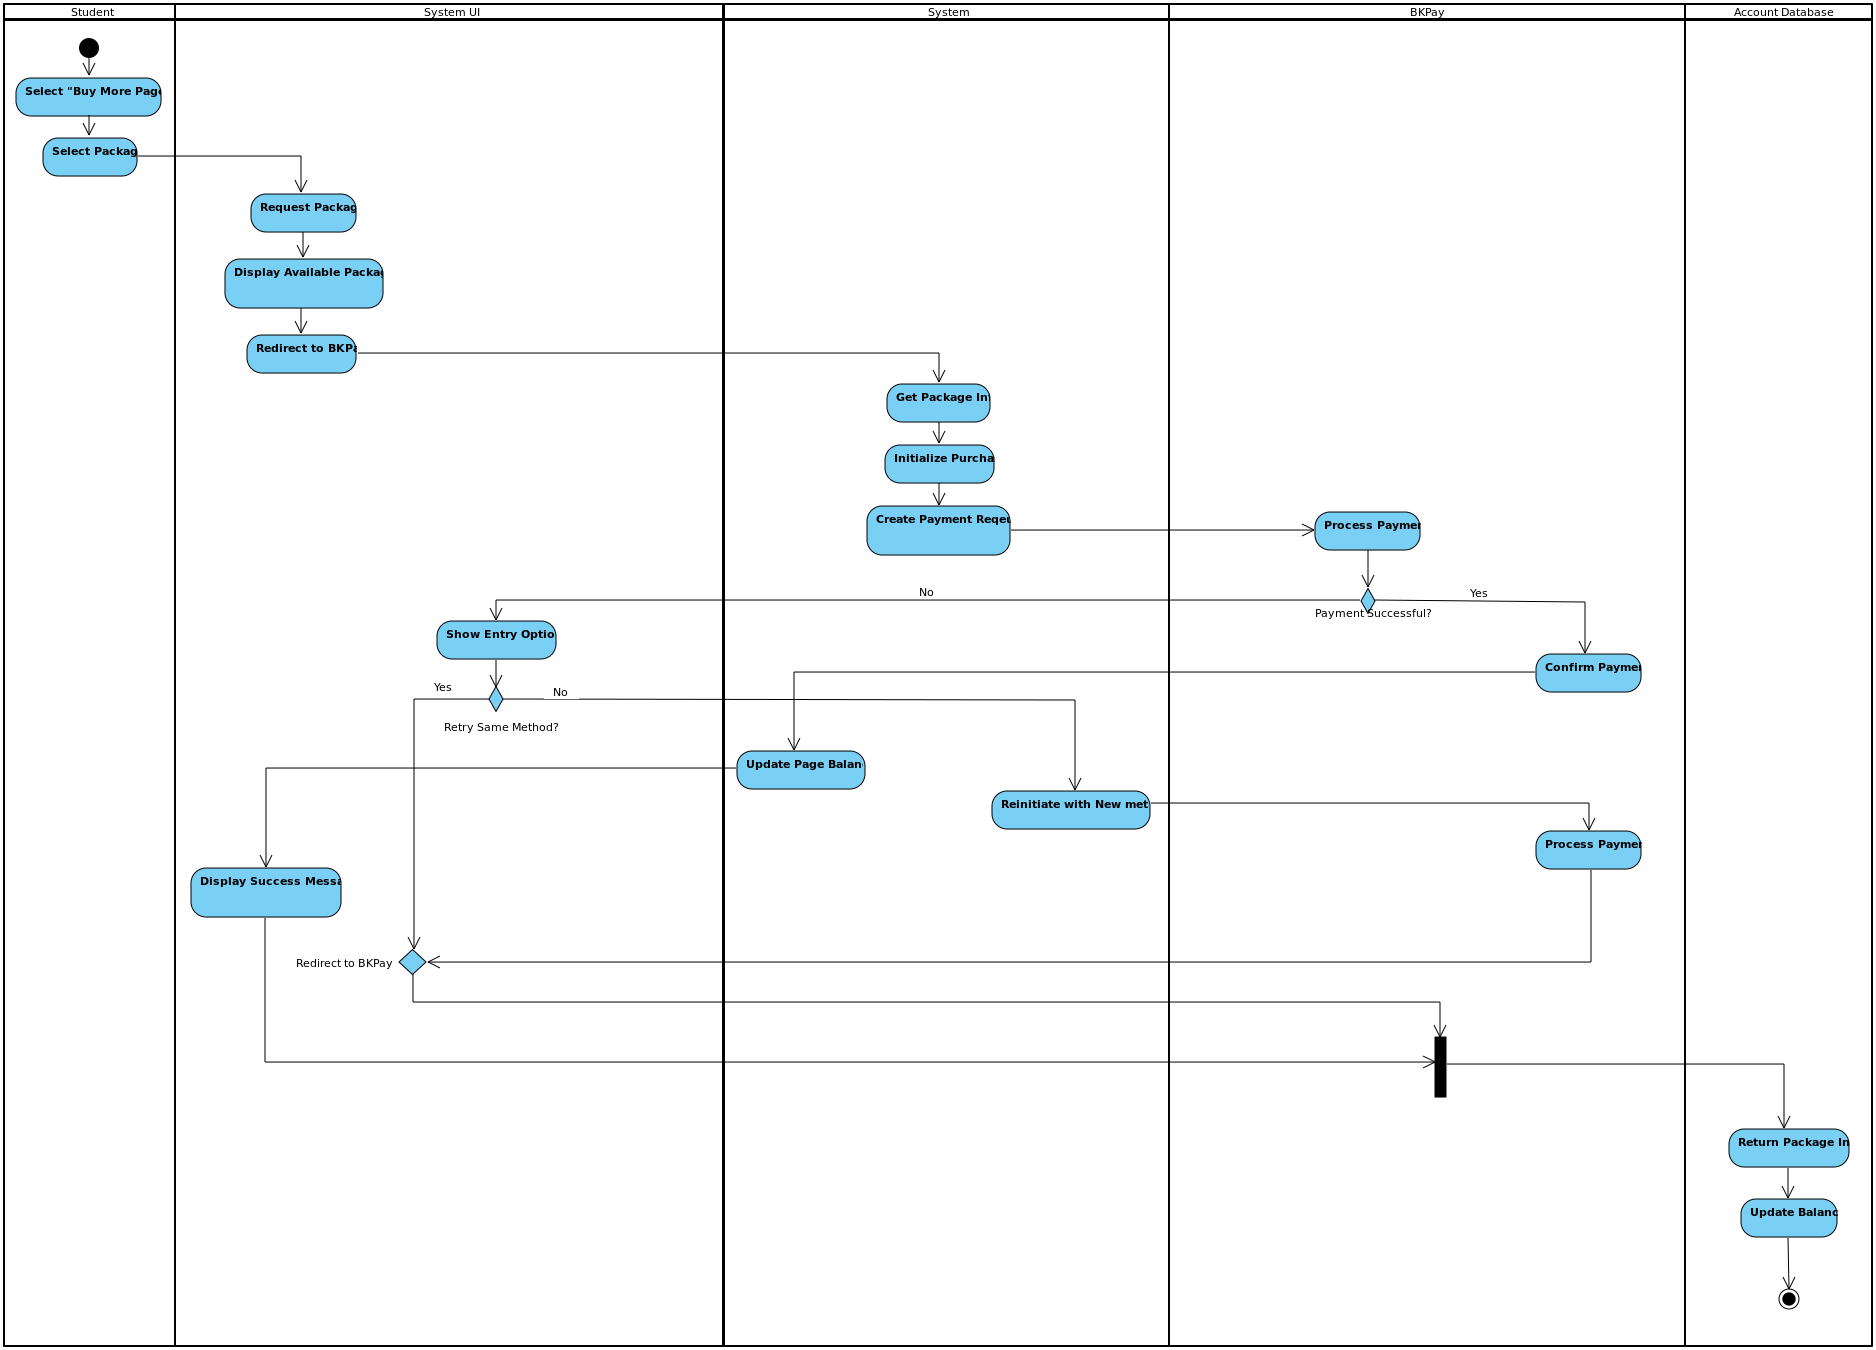
\includegraphics[width = 5in]{activity_diagram/buy_more_pages.png}
    \caption{UseCase - Buy More Pages}
\end{figure}
This diagram outlines the workflow of purchasing additional printing pages in the HCMUT Student Smart Printing Service. The process starts when a student initiates the "Buy More Pages" action, selects a desired package, and is redirected to BKPay for payment processing. After the System retrieves package details and prepares a payment request, the BKPay service processes the payment. If the payment is successful, the System updates the student’s page balance and displays a success message. If the payment fails, the student is given options to retry or select a different payment method. The diagram captures essential decision points, error handling, and system interactions to ensure the smooth completion of the purchase process, helping students conveniently manage their printing needs.

\begin{figure}[H]
    \centering
    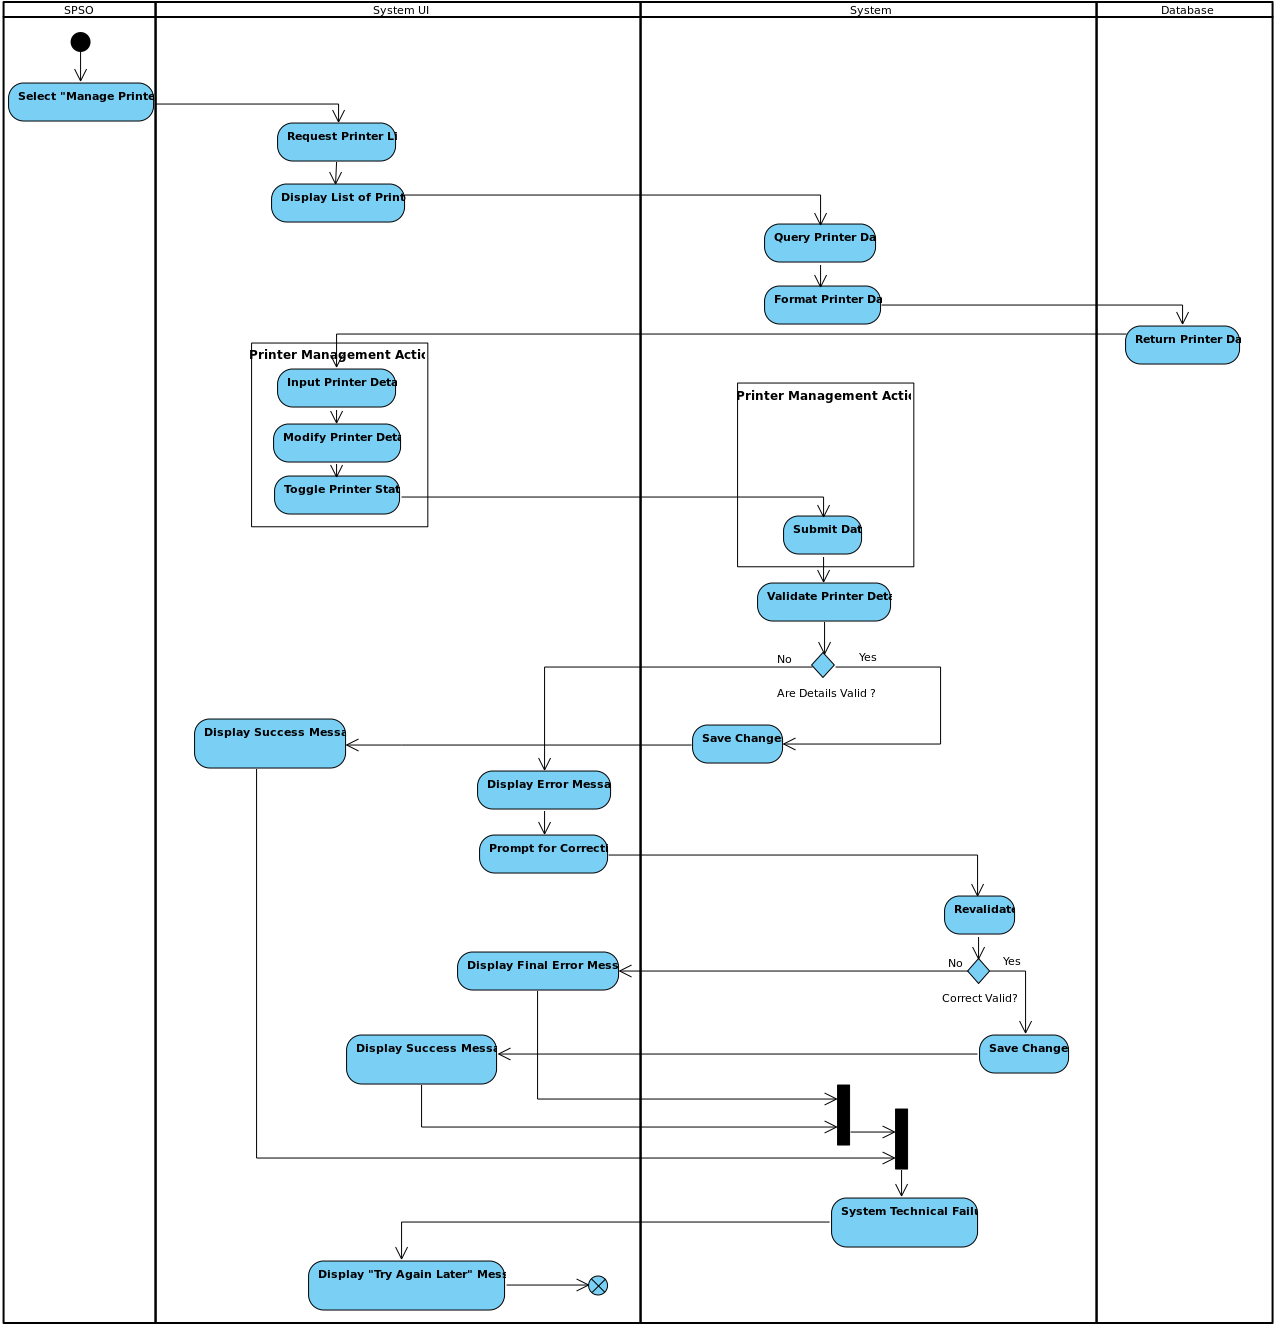
\includegraphics[width = 5in]{activity_diagram/manage_printers.png}
    \caption{UseCase - Manage Printers}
\end{figure}
This diagram illustrates the process of managing printers within the HCMUT Student Smart Printing Service by the Student Printing Service Officer (SPSO).

The process starts when the SPSO selects the "Manage Printers" option. The System UI requests and displays a list of available printers by querying the System and retrieving data from the Database. The SPSO can then perform various printer management actions, such as entering new printer details, modifying existing printer information, or toggling a printer's status (e.g., enabling or disabling a printer).

When the SPSO submits printer information, the System validates the input details. If there are errors, an error message is displayed and the SPSO is prompted to correct the details. If the validation fails repeatedly, a final error message is displayed. Once validated, changes are saved and a success message confirms the update. In case of a technical failure during the process, the system displays a "Try Again Later" message to the SPSO, allowing them to retry at a later time.

This diagram captures the detailed workflow for printer management, including decision points for validation, error handling, and the steps to successfully update printer settings in the system.


\begin{figure}[H]
    \centering
    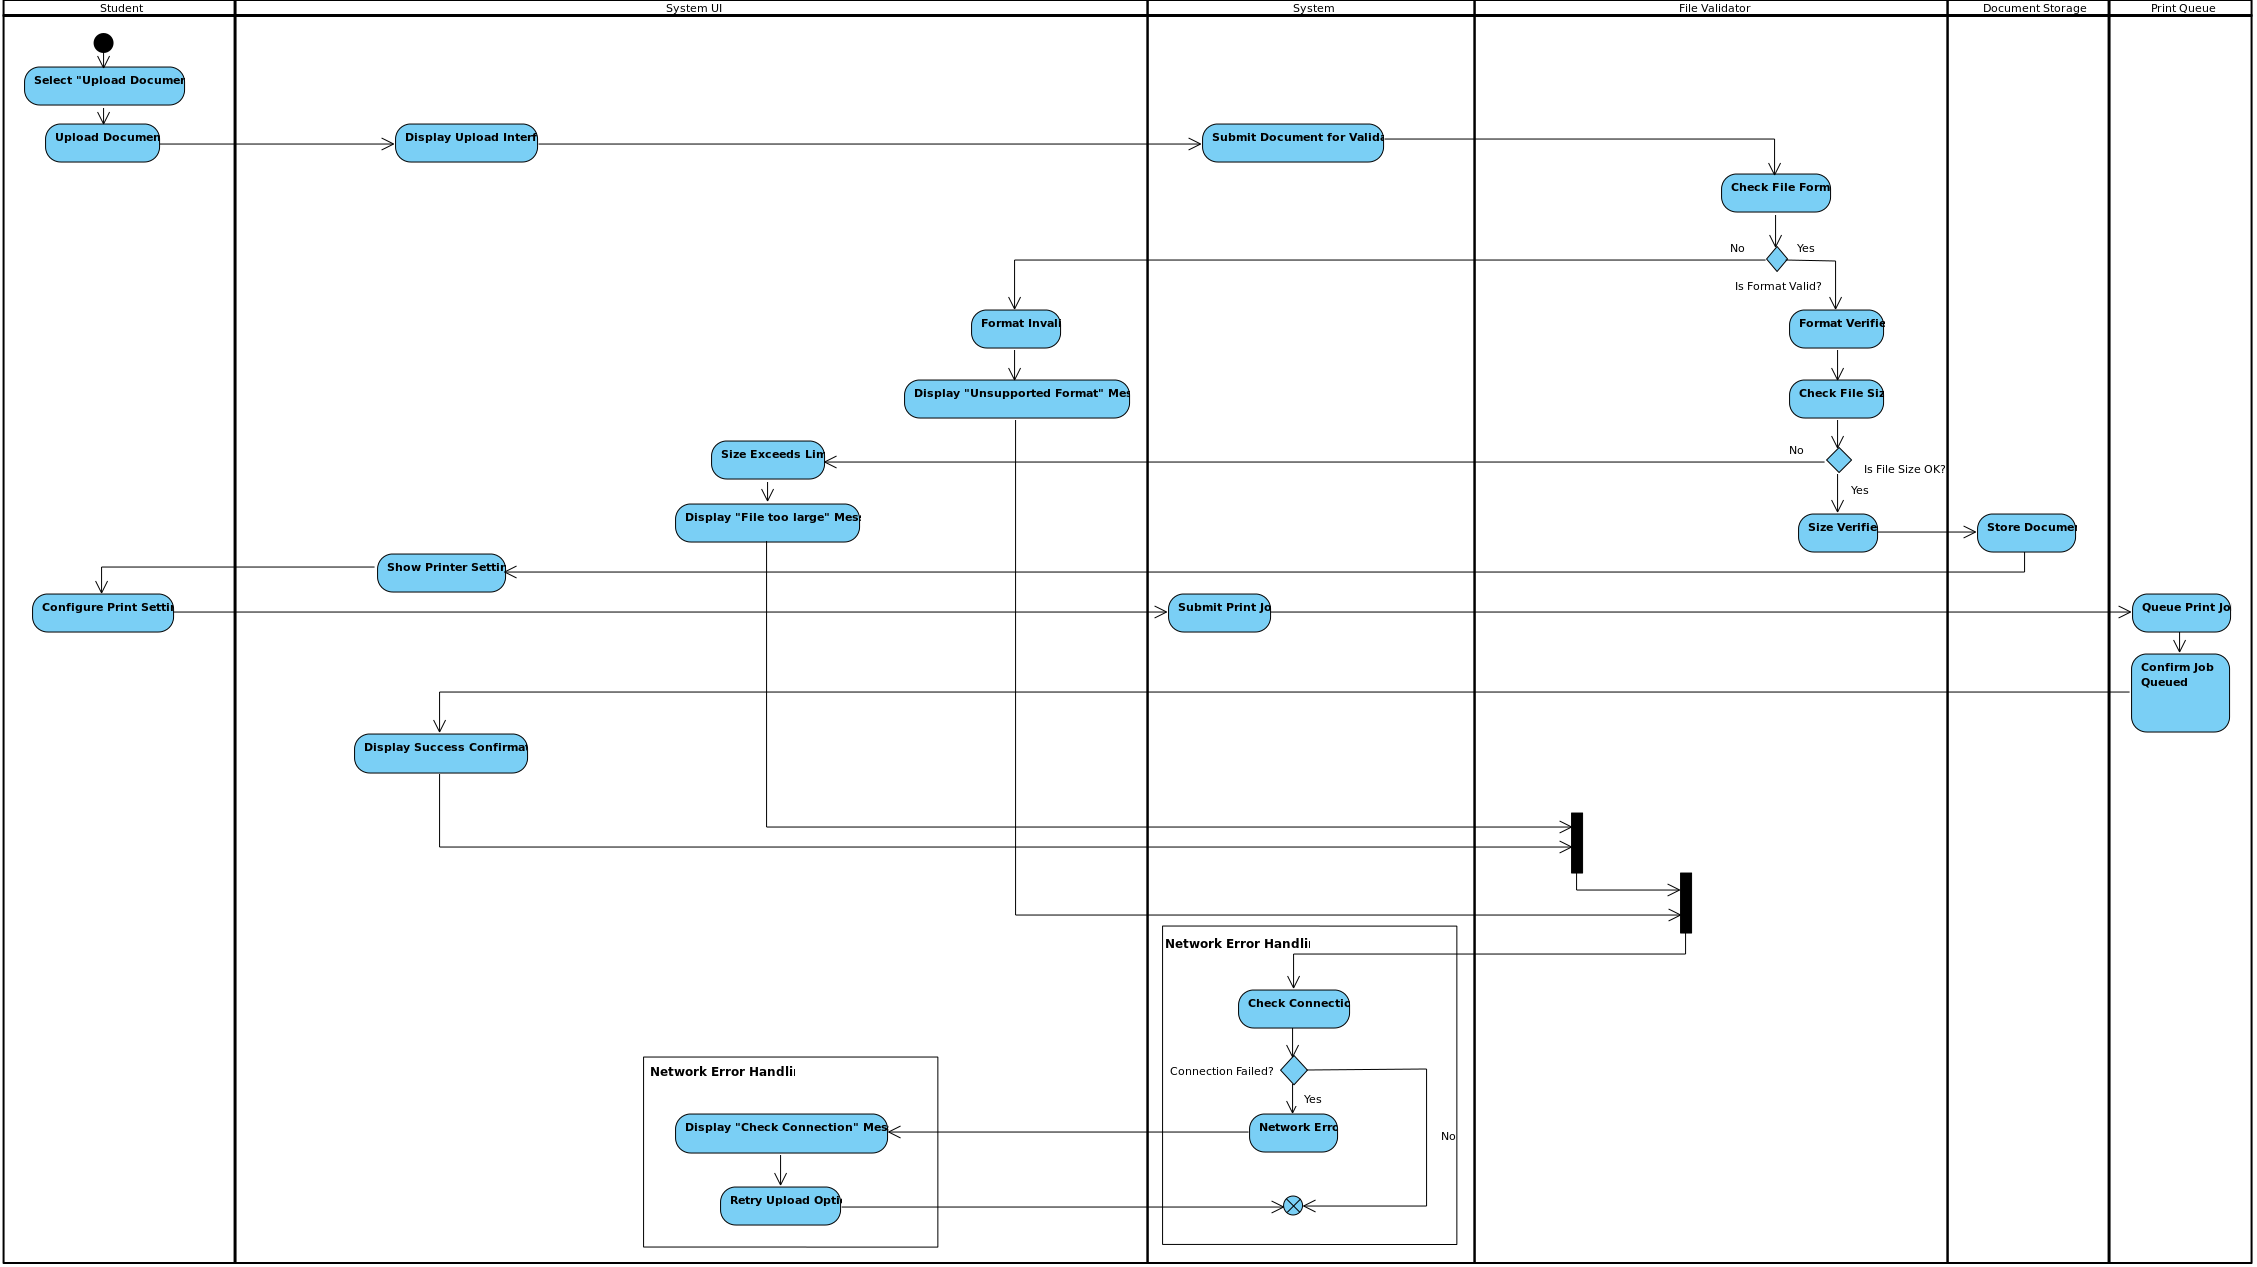
\includegraphics[width = 5in]{activity_diagram/upload_docs.png}
    \caption{UseCase - Upload Docs}
\end{figure}
This Activity Diagram illustrates the document upload and printing process in the HCMUT Student Smart Printing Service. 

The process begins with a Student selecting the "Upload Document" option and uploading their document through the System UI. The System forwards the document to the File Validator to check the file format and size. If the format is unsupported, an "Unsupported Format" message is displayed. If the file size exceeds the limit, a "File Too Large" message is shown, and the student must modify the file before retrying.

Once the file passes validation for both format and size, it is stored in Document Storage. The System UI then allows the student to configure print settings (e.g., paper size, print quality, and copies). After the student confirms the print settings, the System submits the print job to the Print Queue.
The print job is then queued, and a confirmation message is displayed, indicating that the job has been successfully queued for printing. In case of a network error during upload, the Network Error Handling process prompts the student to check their connection and retry the upload.

This diagram captures essential decision points, validation steps, and error-handling mechanisms to ensure a smooth and efficient document upload and printing process for students.

\begin{figure}[H]
    \centering
    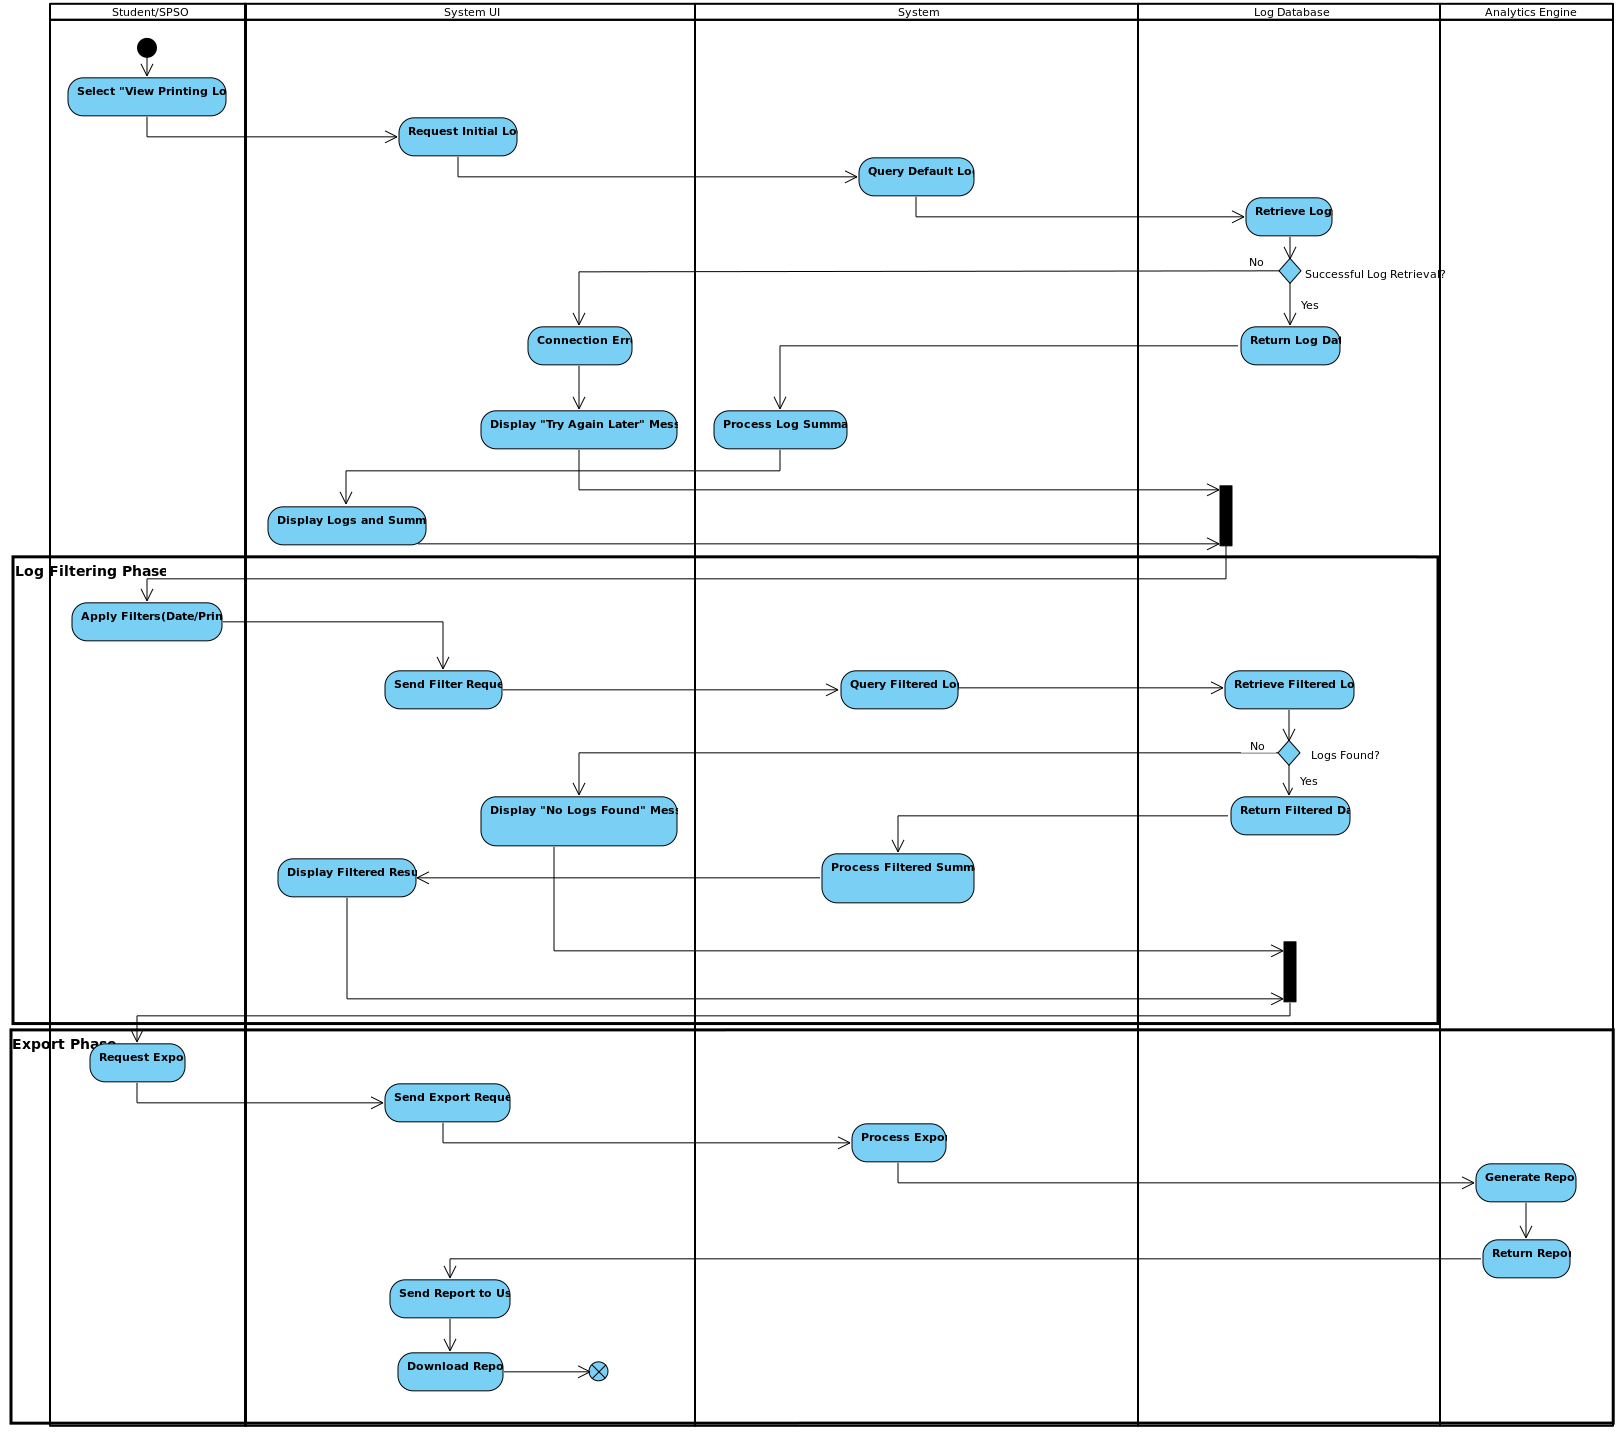
\includegraphics[width = 5in]{activity_diagram/view_printing_logs.png}
    \caption{UseCase - View Printing Logs}
\end{figure}
This Activity Diagram illustrates the process of viewing, filtering, and exporting printing logs within the HCMUT Student Smart Printing Service. Both Students and Student Printing Service Officers (SPSO) can access this feature.
\begin{enumerate}
    \item The process begins when a user selects "View Printing Logs." The System UI requests the initial logs, and the System queries the Log Database for default log data. If retrieval is successful, the logs and a summary are displayed. If there is a connection error, an error message prompts the user to try again later.
    \item In the Log Filtering Phase, the user applies specific filters (such as date, printer ID, or student ID). The System processes the filter request, queries the Log Database for the filtered data, and checks if any logs match the filters. If no logs are found, a "No Logs Found" message is displayed; otherwise, the filtered results and summary are shown.
    \item In the Export Phase, the user can request an export of the filtered or full log data. The System processes this request and generates a report through the Analytics Engine. The generated report is then made available for download, allowing the user to retrieve a detailed log record.
\end{enumerate}
This diagram captures the steps, decision points, and error-handling mechanisms involved in accessing and managing printing logs, giving users flexible options to view, filter, and export data as needed.


\section{Sequence Diagram}

\subsection{Usecase Login}

\vspace{1cm}

\begin{figure}[H]
    \vspace{-0.5cm}
    \centering
    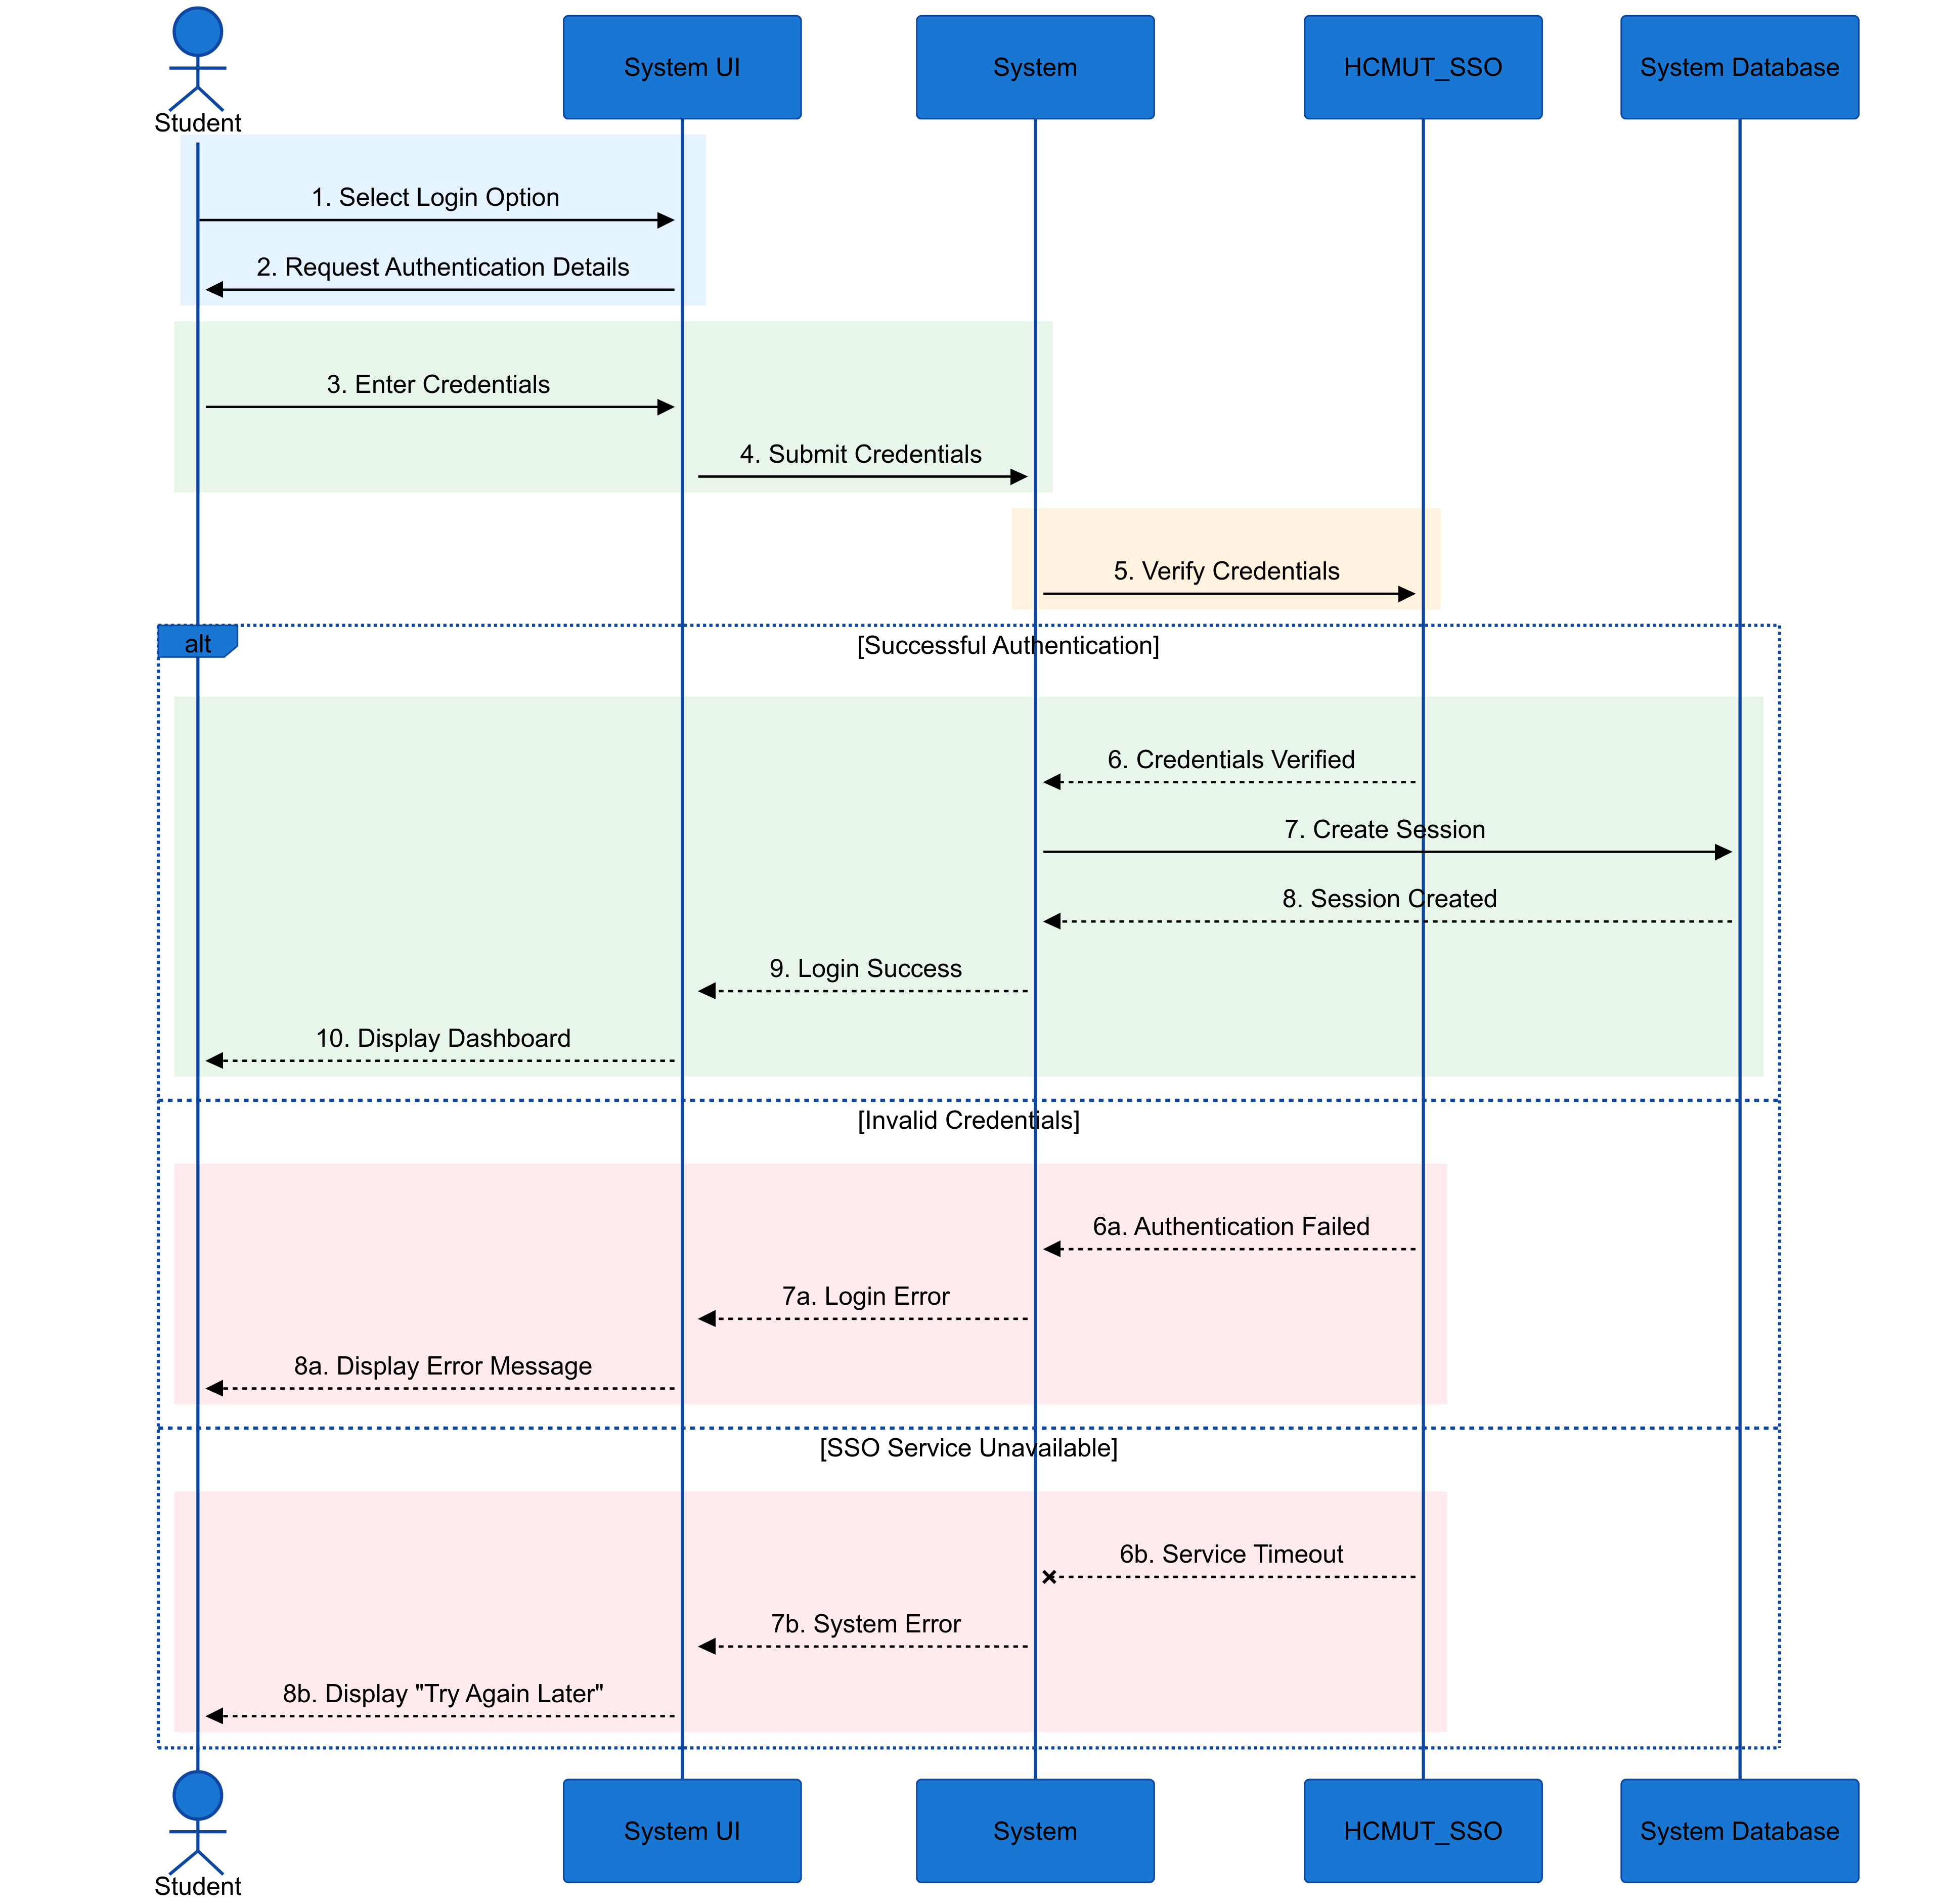
\includegraphics[width=0.85\textwidth]{images/sequence_diagram/Login.png}
    \caption{UseCase - Login}
    \label{fig:login}
\end{figure}


This sequence diagram describes the "Login" use case, where a student logs into a system via a single sign-on (SSO) service. The process starts when the student selects the login option on the system UI, prompting the system to request authentication details. The student enters their credentials, which are submitted to the SSO (HCMUT$\_$SSO) for verification.

If the credentials are correct, the SSO service verifies them, initiates a session creation request, and once the session is created, returns a success message to the system. The system then displays the main dashboard, indicating a successful login.

If the credentials are invalid, the SSO service responds with an authentication failure, prompting the system to display an error message indicating incorrect login details. Alternatively, if the SSO service is unavailable (e.g., due to a timeout), the system displays a "Try Again Later" message, informing the student of the temporary issue. This diagram comprehensively outlines the login flow, covering successful login, invalid credentials, and service unavailability scenarios, ensuring that the student receives appropriate feedback in each case.

\subsection{Usecase Doc Upload}

\begin{figure}[H]
    \centering
    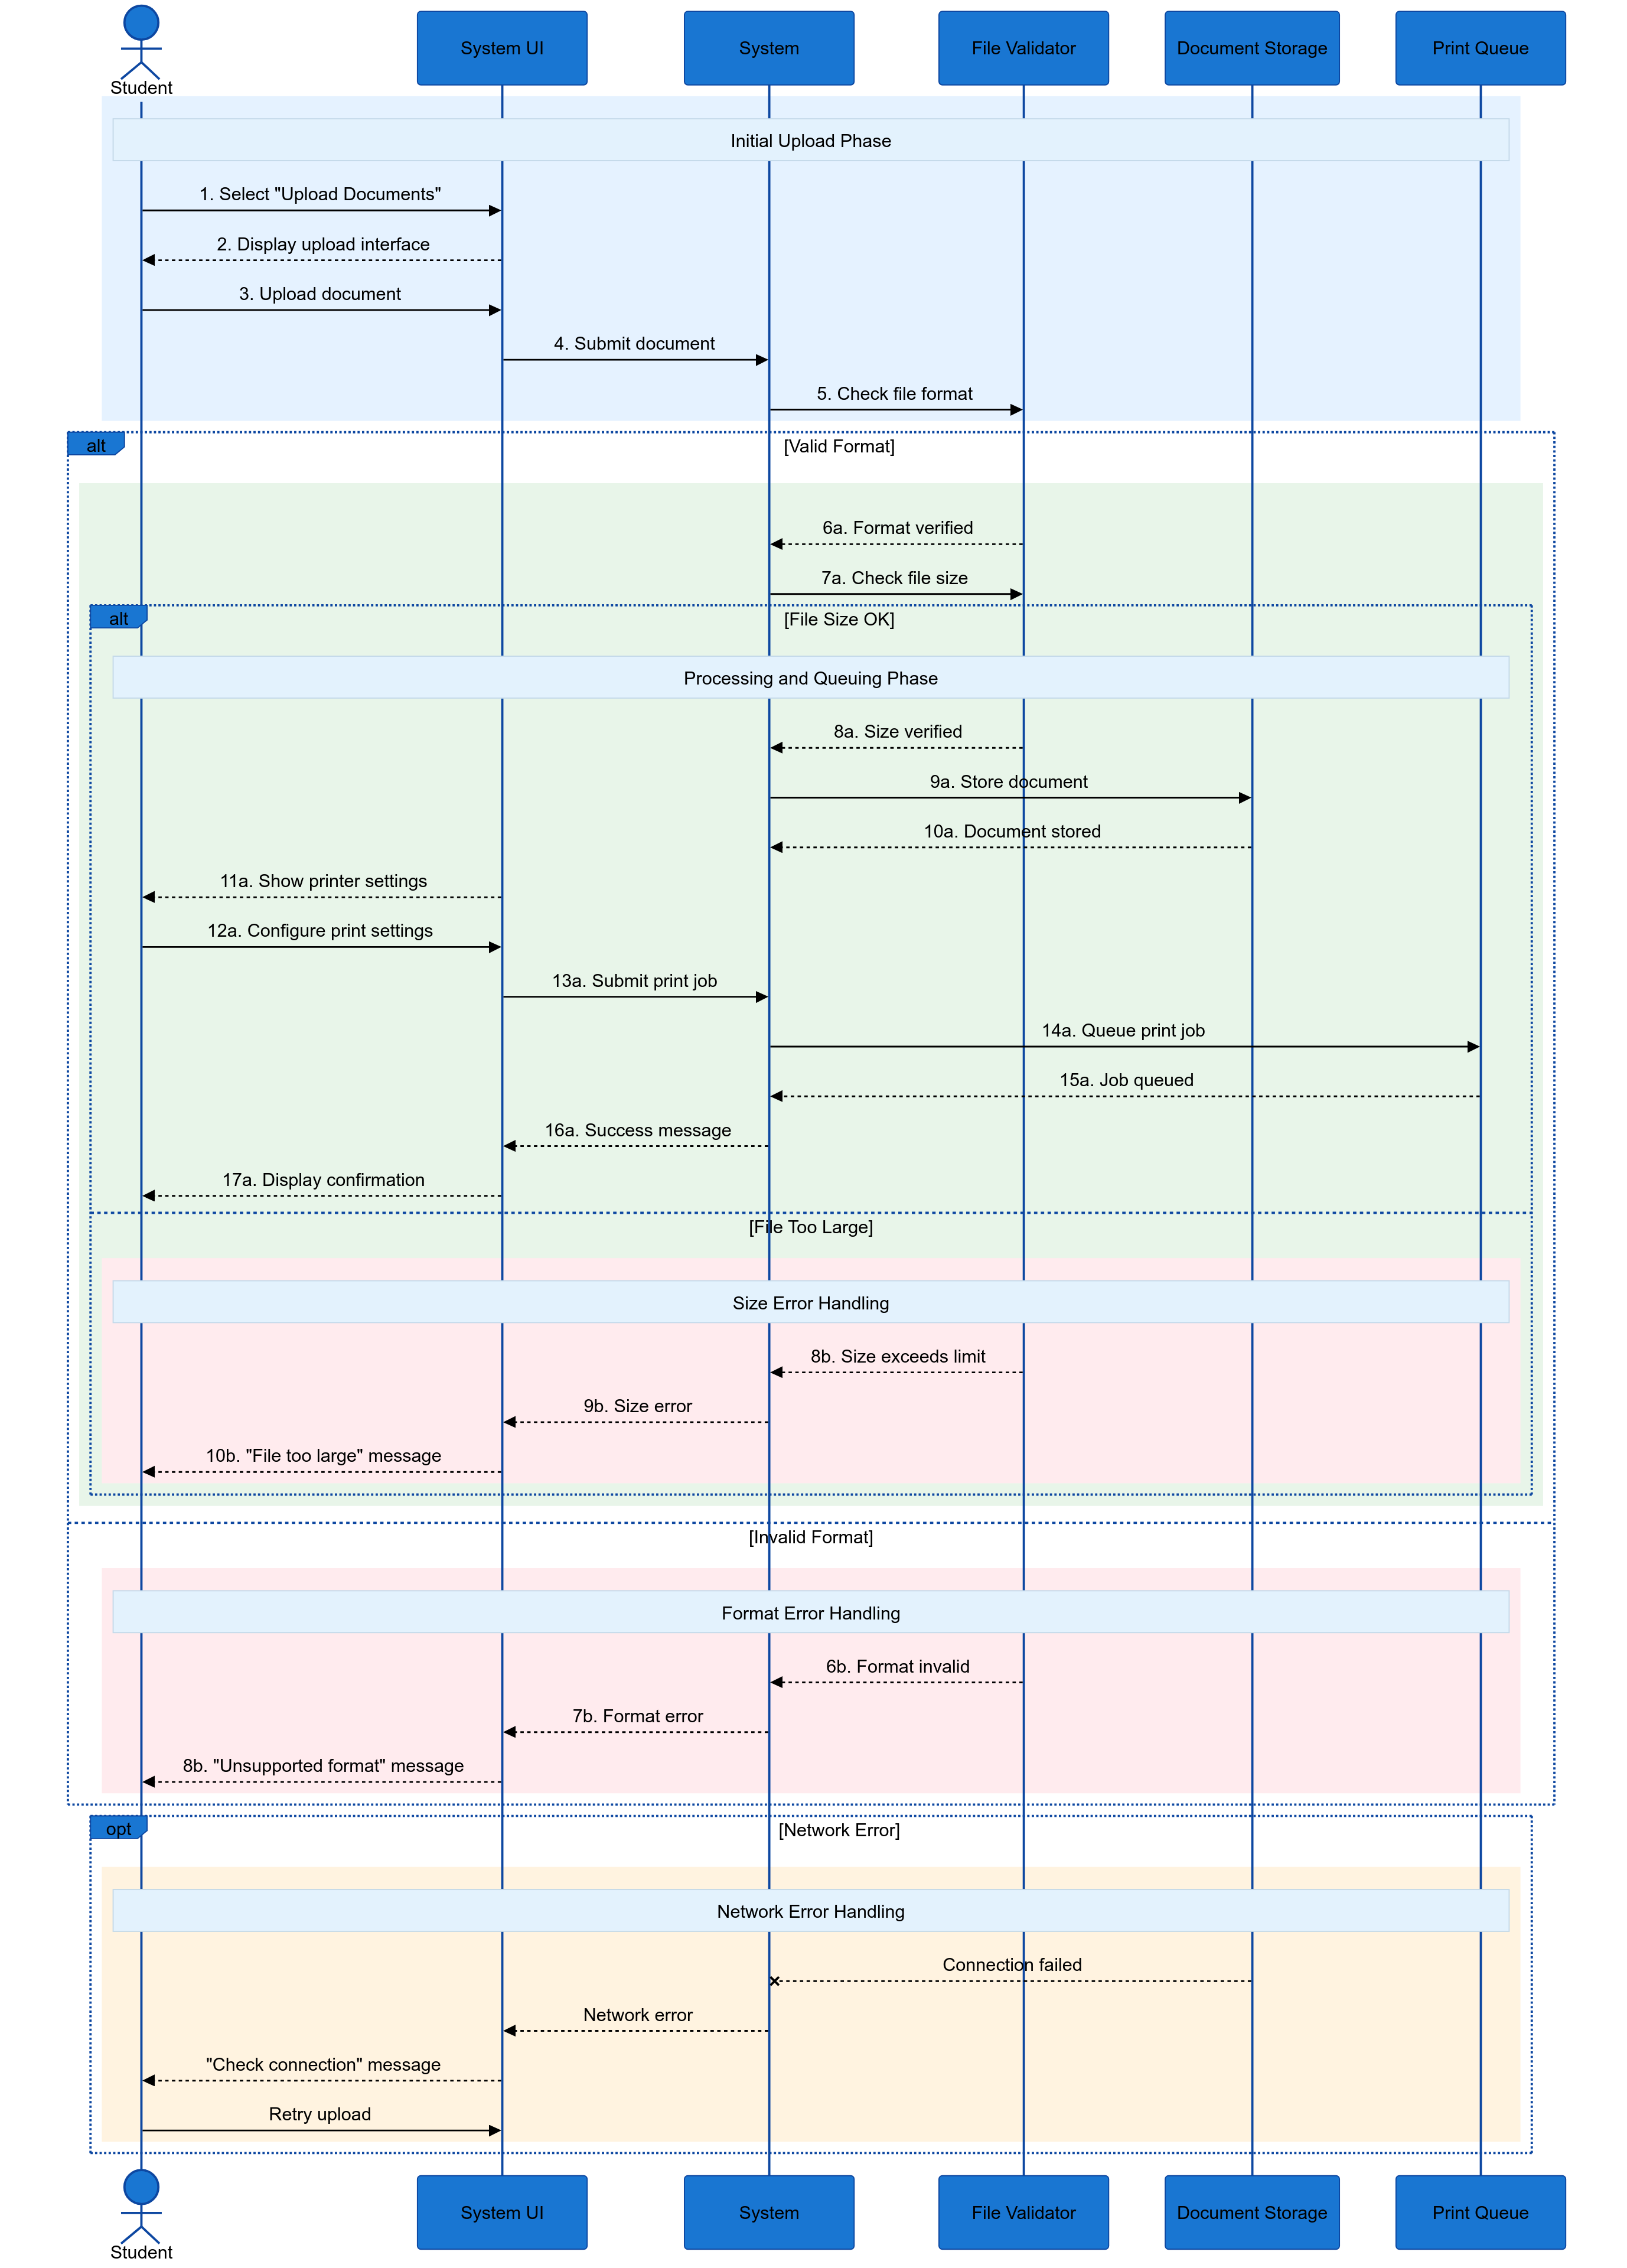
\includegraphics[width=0.9\textwidth]{images/sequence_diagram/Upload Doc.png}
    \caption{UseCase - Doc Upload}
    \label{fig:upload_doc}
\end{figure}

The diagram illustrates the "Upload Document" process, where a student begins by selecting "Upload Documents" on the UI. The student uploads a document, which is submitted to the file validator. If both the format and size are acceptable, the document is stored in the document storage system. The system then prompts the student with printer settings, allowing them to configure print options before submitting the print job. Once submitted, the document is queued, a success message is displayed to the student. If the file format or size is invalid, appropriate error messages ("Unsupported format" or "File too large") are displayed, notifying the student of the issue. In case of a network error, a "Check connection" message is shown.


% \begin{figure}[H]
%     \centering
%     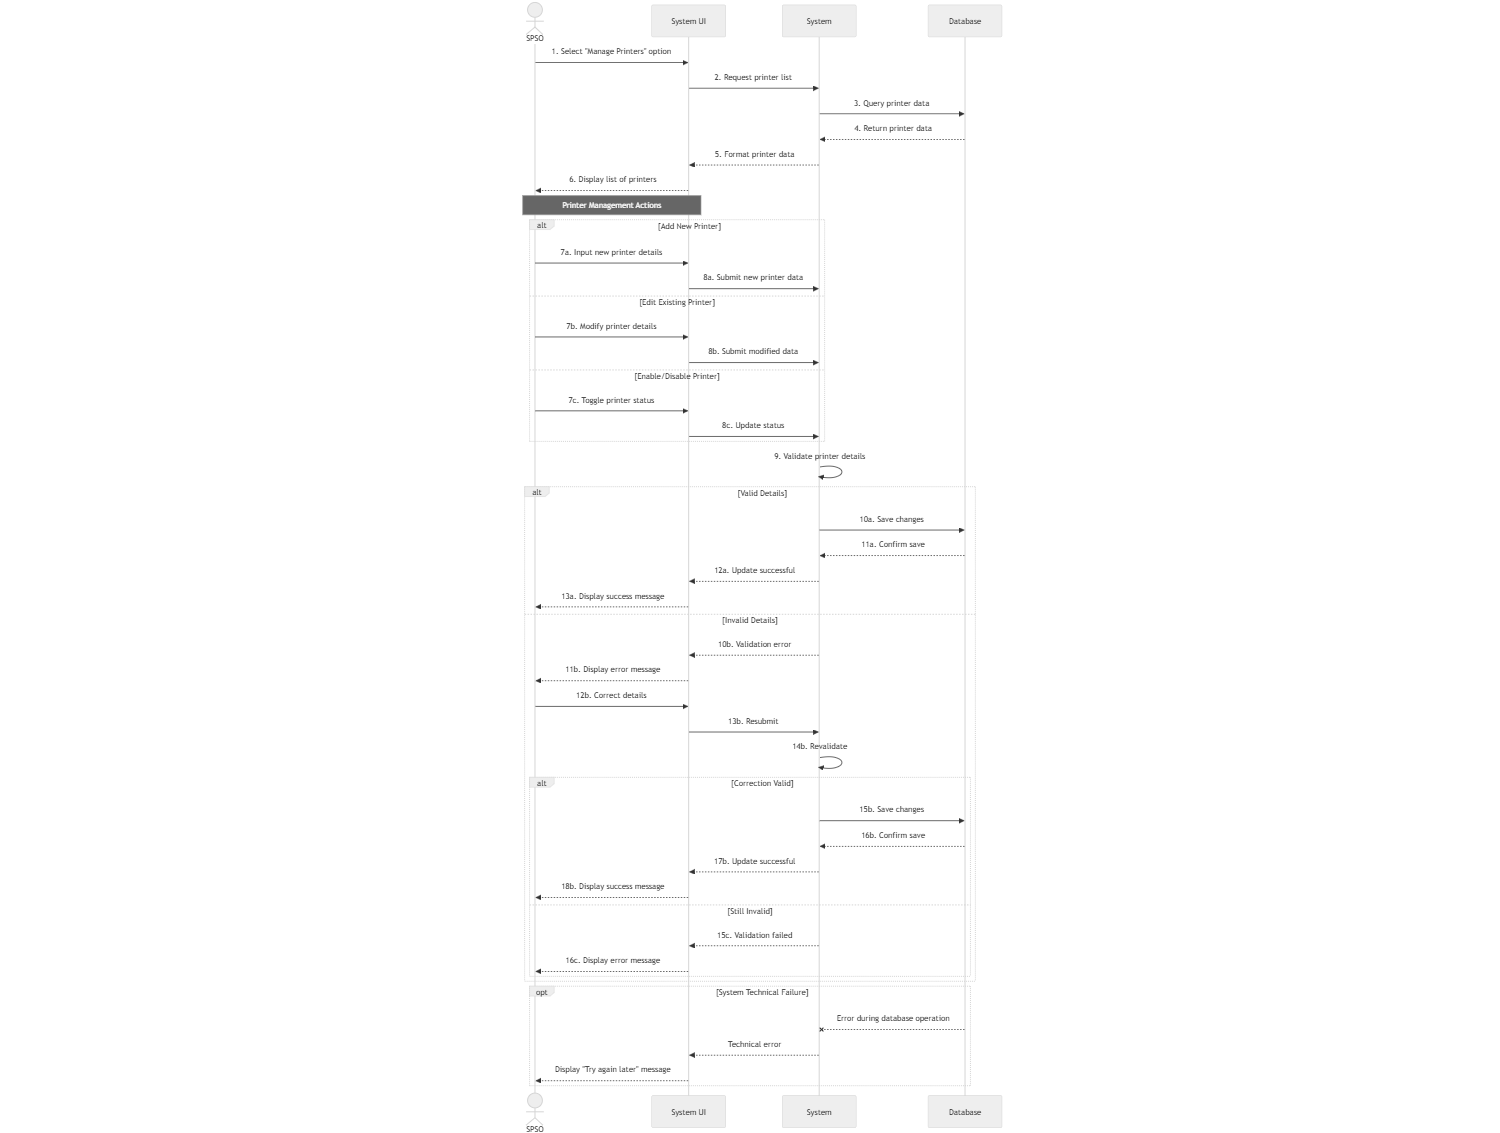
\includegraphics[width = 5in]{UseCase - Manage Printer.png}
%     \caption{UseCase - Manage Printer}
% \end{figure}

\subsection{Usecase Manage Printer}

\begin{figure}[H]
    \centering
    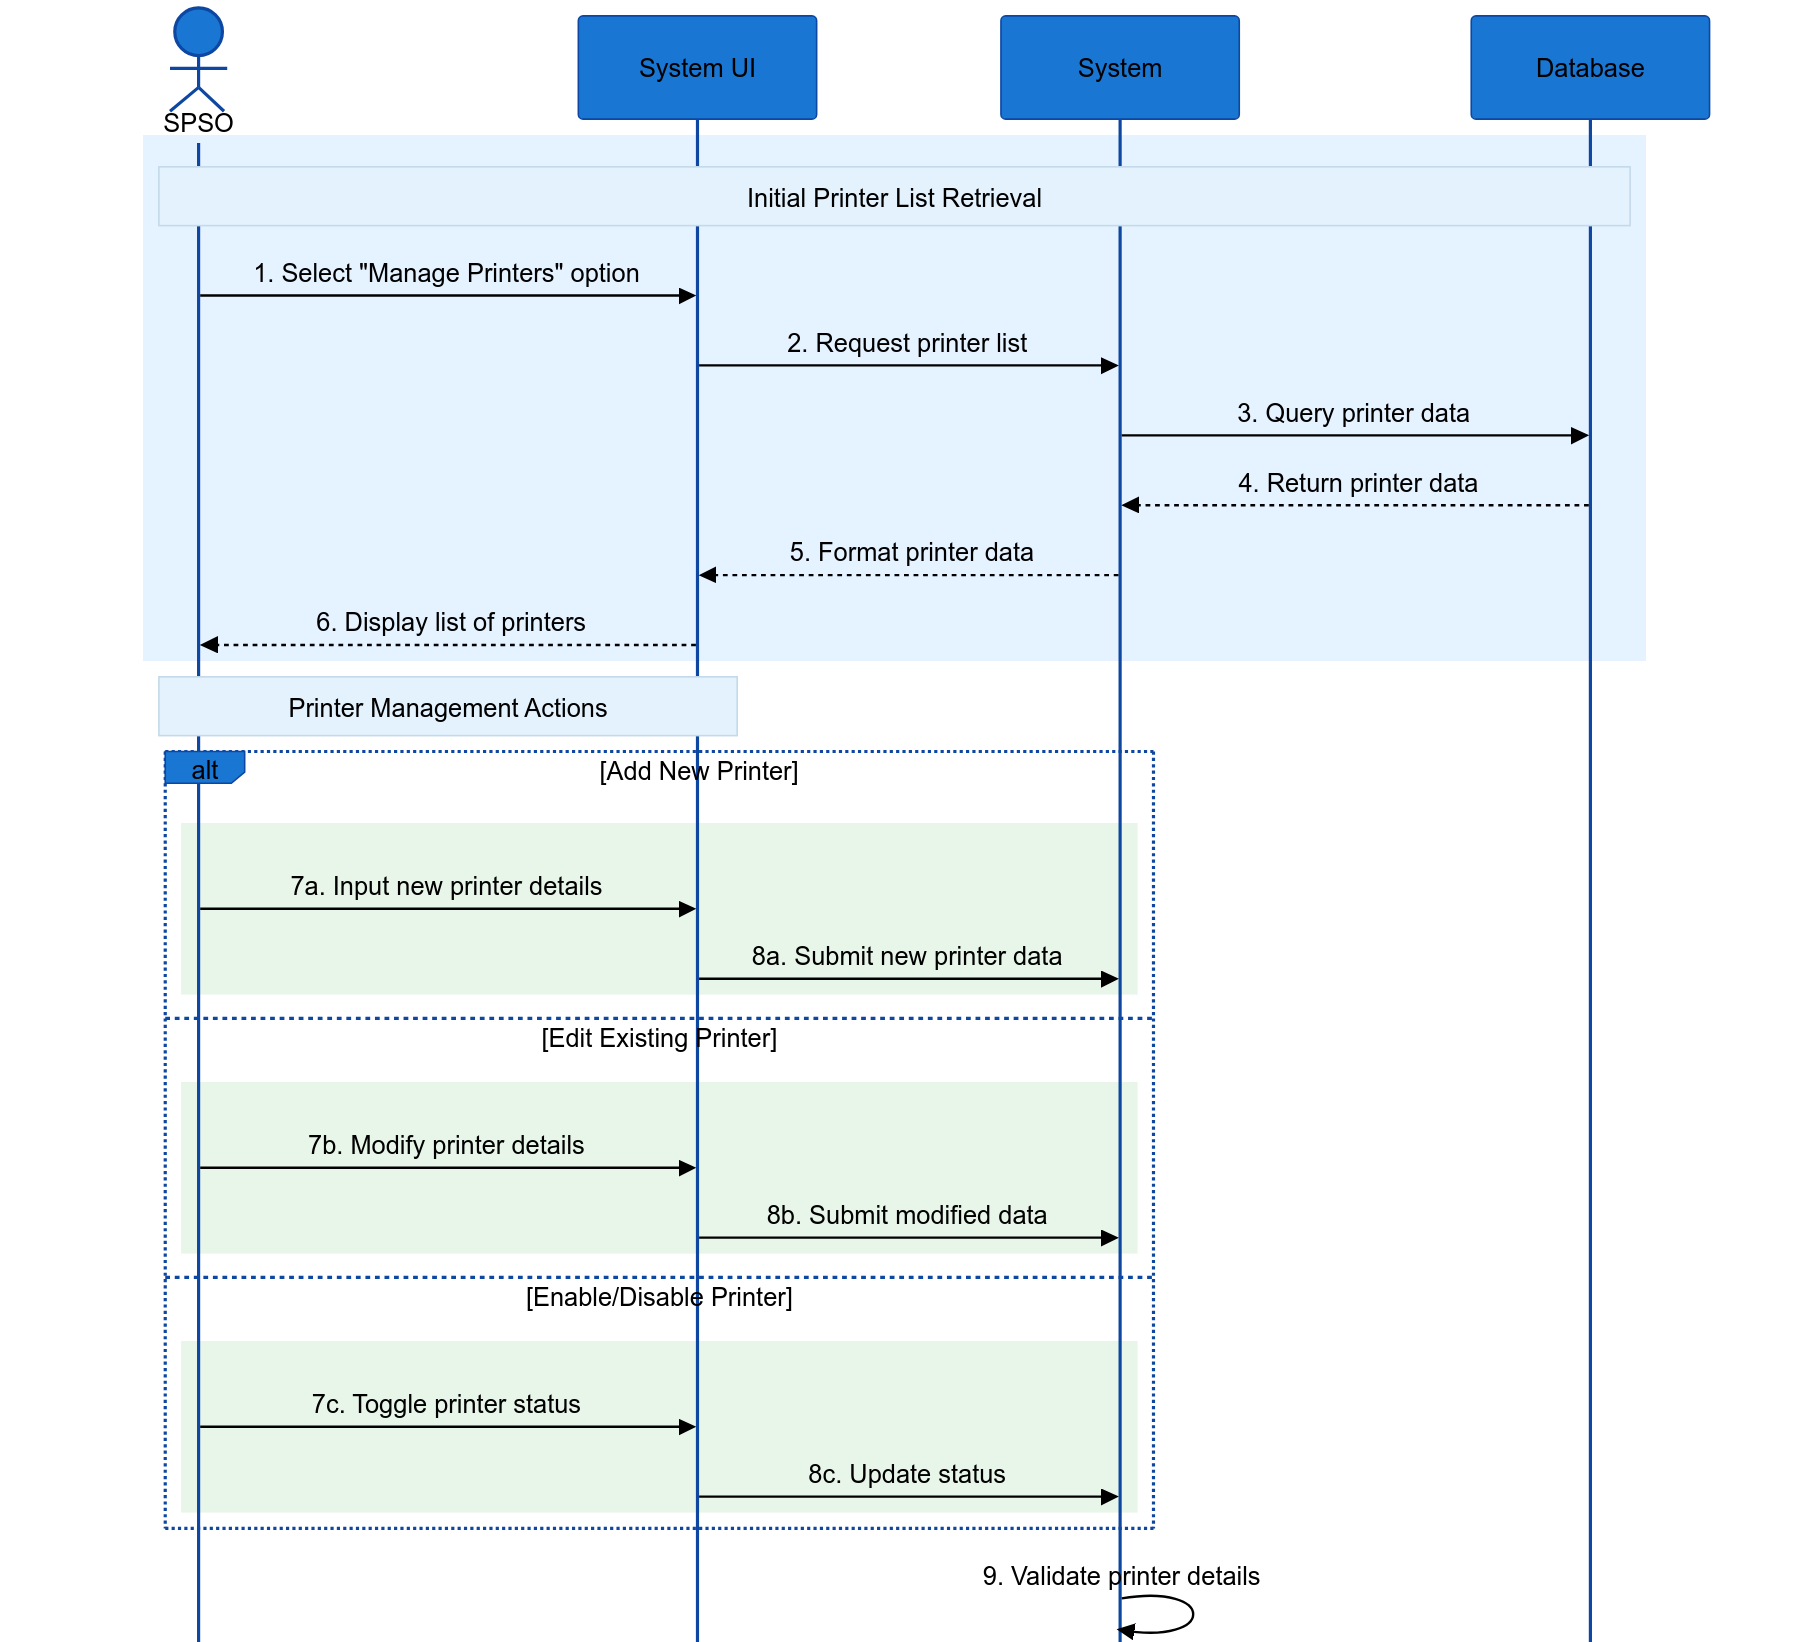
\includegraphics[width=\textwidth ]{images/sequence_diagram/Manage Printers_1.png}
    \label{fig:manage_printer}
\end{figure}

\small \textit{*Notes}: being not fit in a single page, the diagram continues on the next page.

\normalsize

\begin{figure}[H]
    \centering
    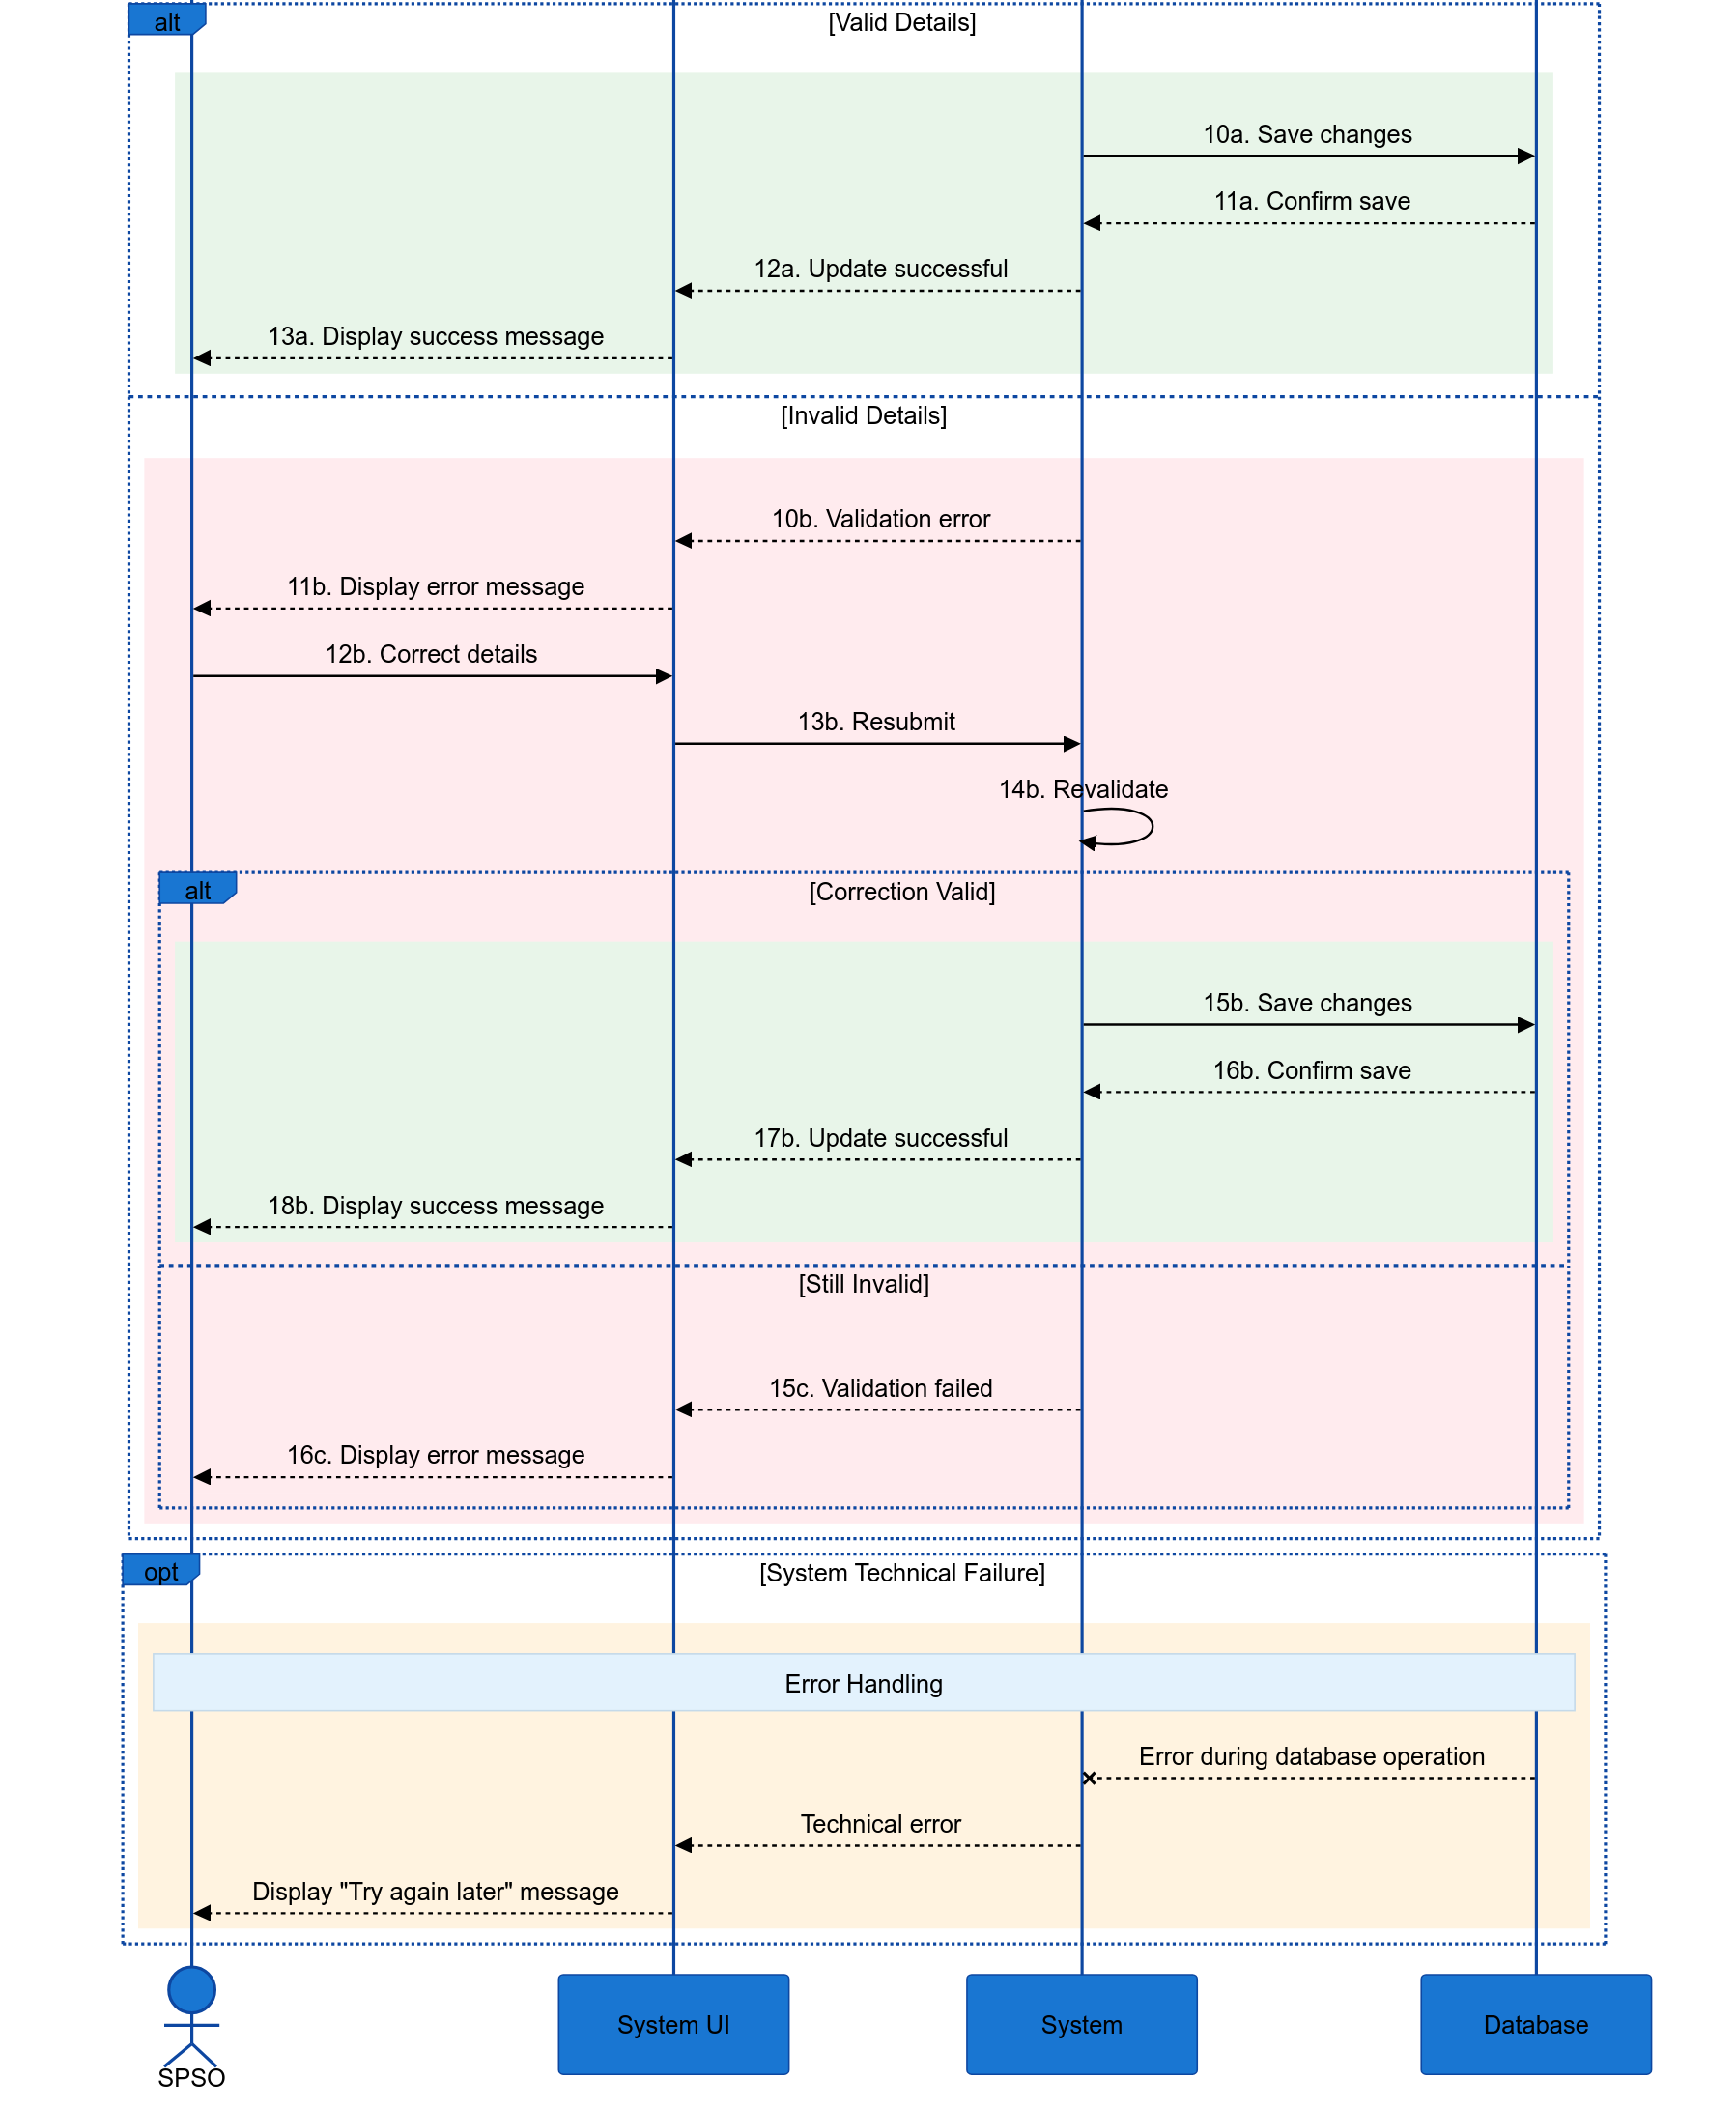
\includegraphics[width=0.9\textwidth ]{images/sequence_diagram/Manage Printers_2.png}
    \caption{UseCase - Manage Printer}
    \label{fig:manage_printer}
\end{figure}

The diagram details the "Manage Printers" usecase, where an SPSO manages printer settings in a system. The process starts when SPSO clicks "Manage Printers", prompting the system to request and retrieve the printer list from the database. The system then displays the list of printer management actions, which can include adding a new printer, editing an existing printer, or enabling/disabling a printer.

In the flow \textbf{Add New Printer}, the SPSO inputs new printer details, submits them, and the system validates the information before committing it to the database. 
In the flow \textbf{Edit Existing Printer}, the SPSO modifies printer details, submits the changes, and the system validates the information before saving. 
In the flow \textbf{Enable/Disable Printer}, the SPSO toggles the printer status, and the system updates this change in the database. In all flows, the system returns a success message if valid.

If any information is invalid during validation, an error message is displayed, prompting the SPSO to correct and resubmit the details. If validation fails again or if there's a technical error during database operations, the system displays relevant error messages ("Try again later") to inform the SPSO of the issue. This sequence covers various printer management operations, ensuring error handling, validation, and system feedback for a seamless user experience.


\subsection{Usecase Buy More Page}

\begin{figure}[H]
    \centering
    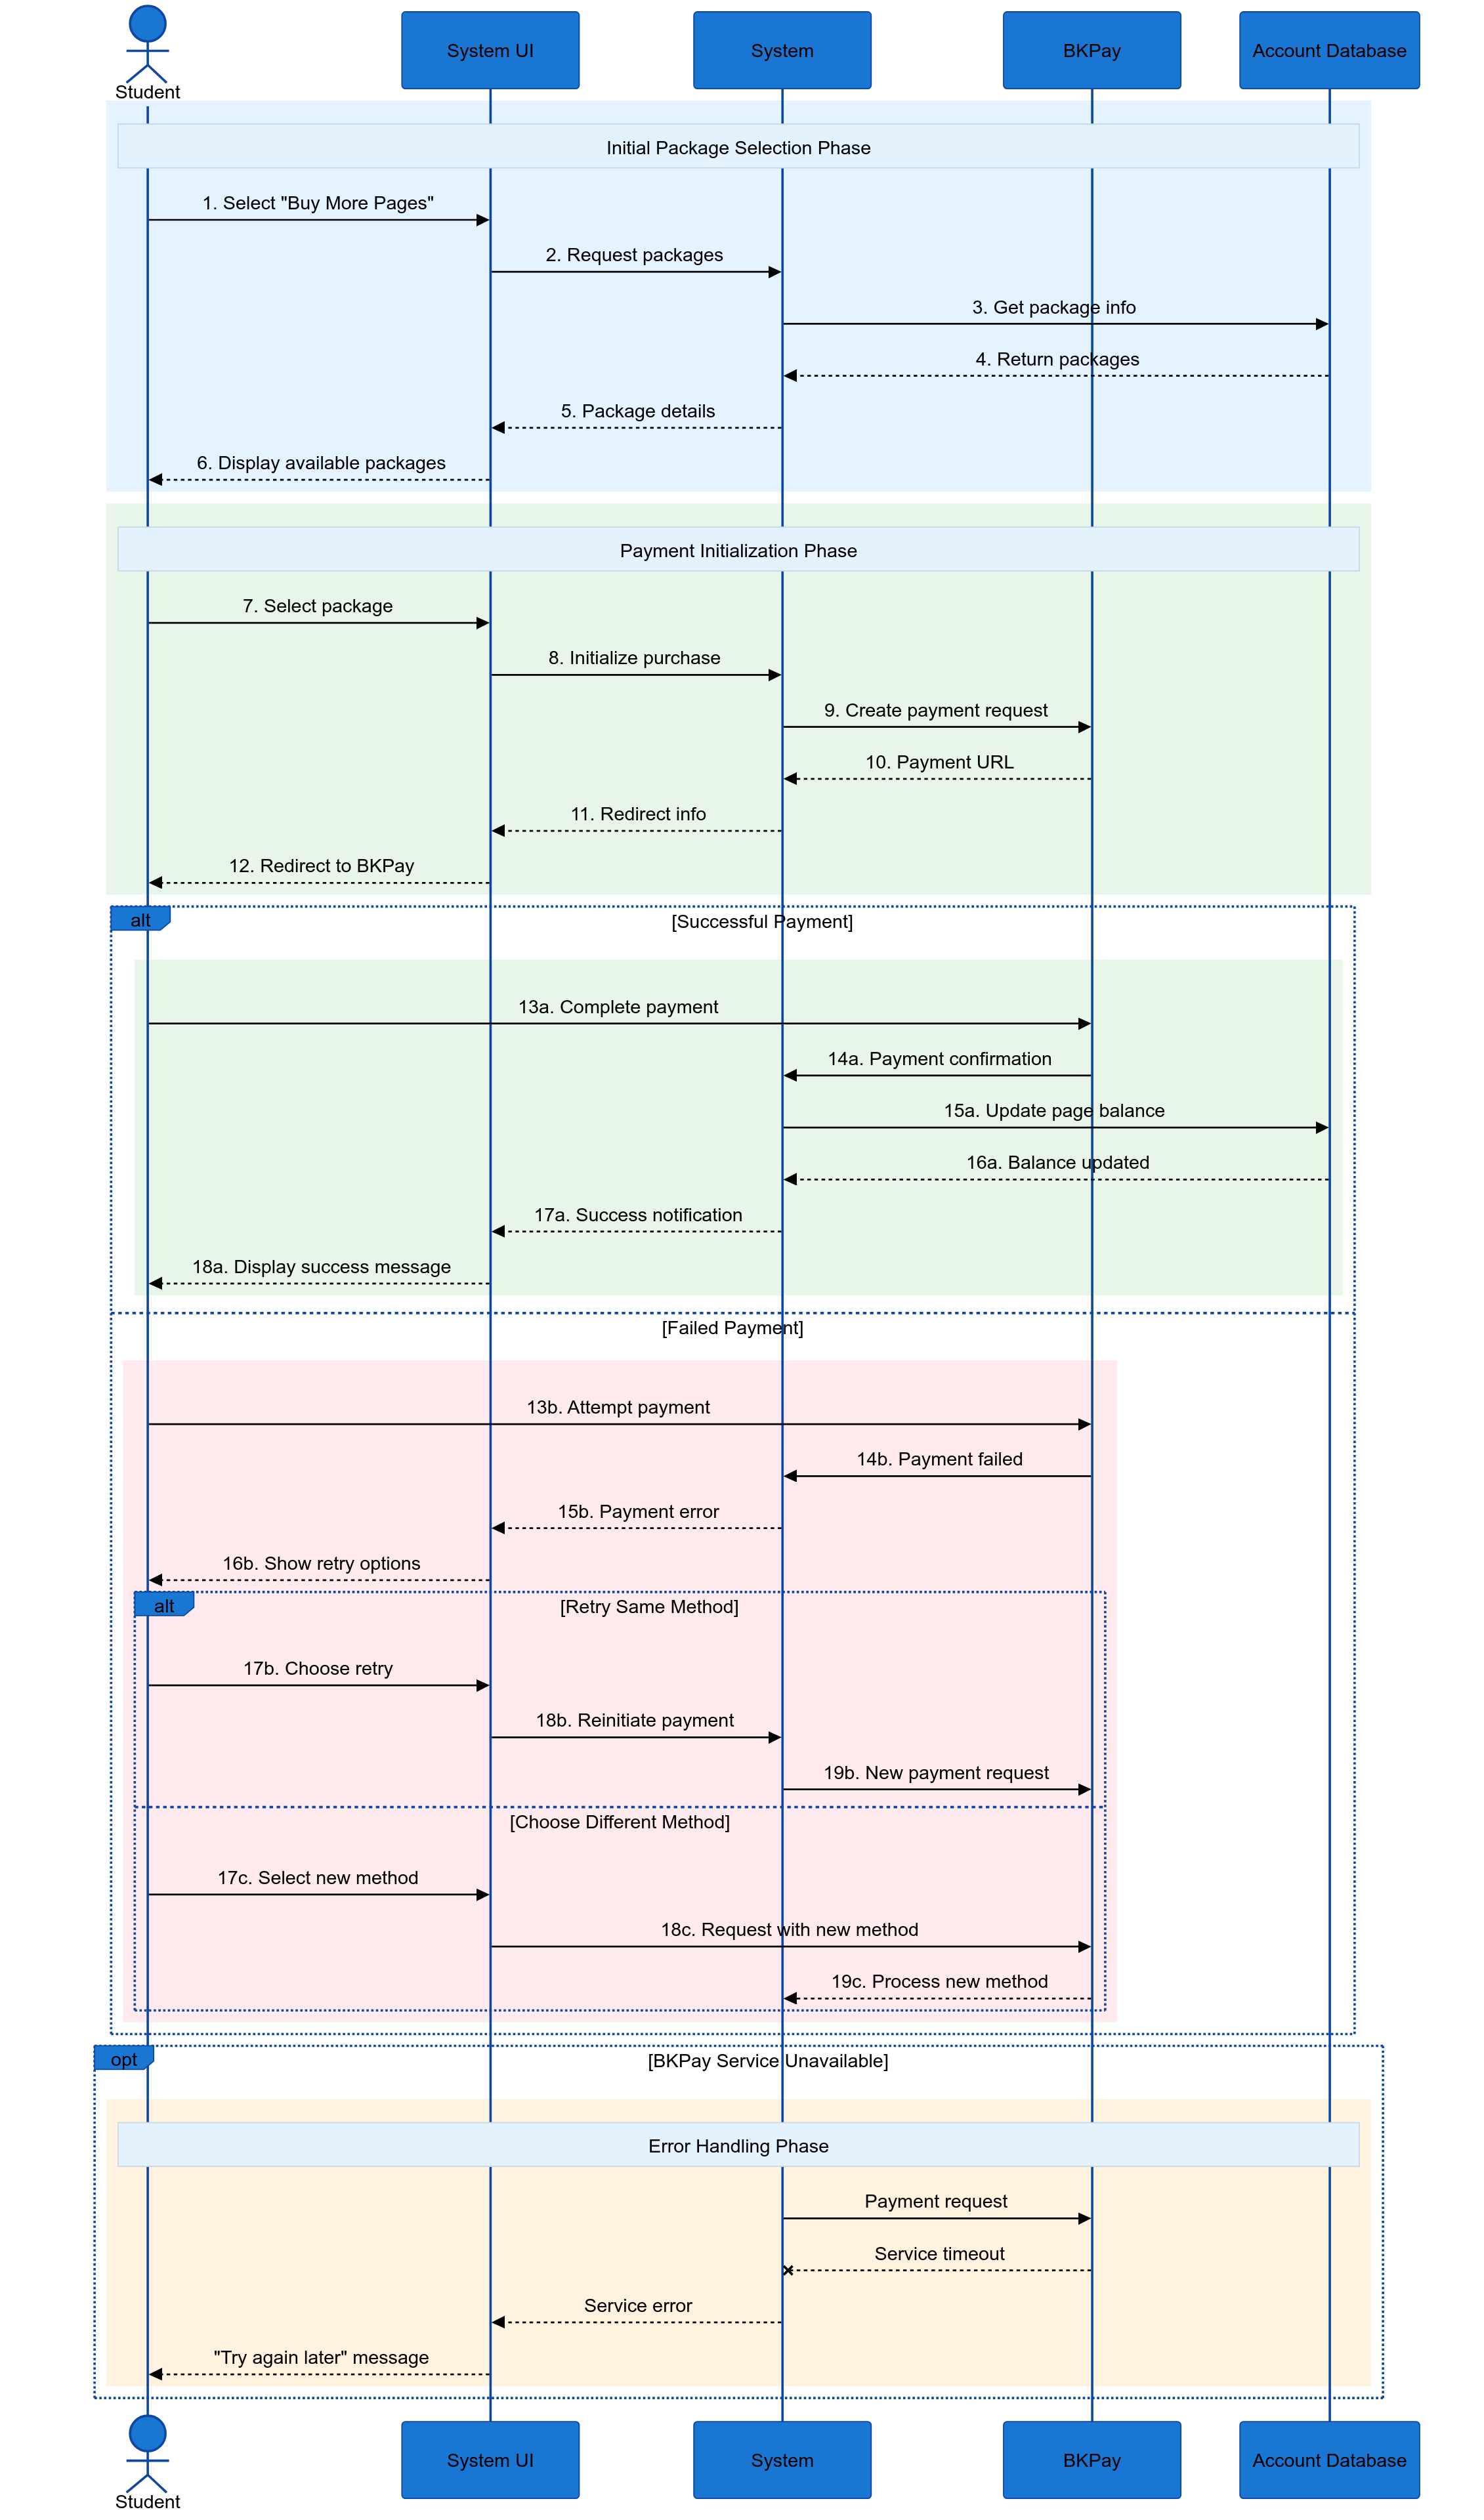
\includegraphics[width=0.8\textwidth]{images/sequence_diagram/Buy More Pages.png}
    \caption{UseCase - Buy More Page}
    \label{fig:buy_more_page}
\end{figure}

This sequence diagram outlines the "Buy More Pages" process, where a student initiates a request by selecting "Buy More Pages" on the system UI. The system retrieves available packages and displays them to the student, who then selects a desired package. Upon package selection, a purchase request is sent to the payment gateway (BKPay), which initializes the payment process and redirects the user for payment. If the payment is successful, a confirmation is sent to the system, which then updates the student's page balance in the account database and displays a success message. In case of payment failure, the system provides retry options, allowing the student to either retry with the same method or choose a different payment method. If the payment gateway service is temporarily unavailable, a "Service error" message is displayed, and the student is advised to "try again later." This diagram ensures a comprehensive understanding of the "Buy More Pages" process, covering successful transactions, error handling, and retry options to enhance user experience.

\subsection{Usecase View Printing Logs}

\begin{figure}[H]
    \centering
    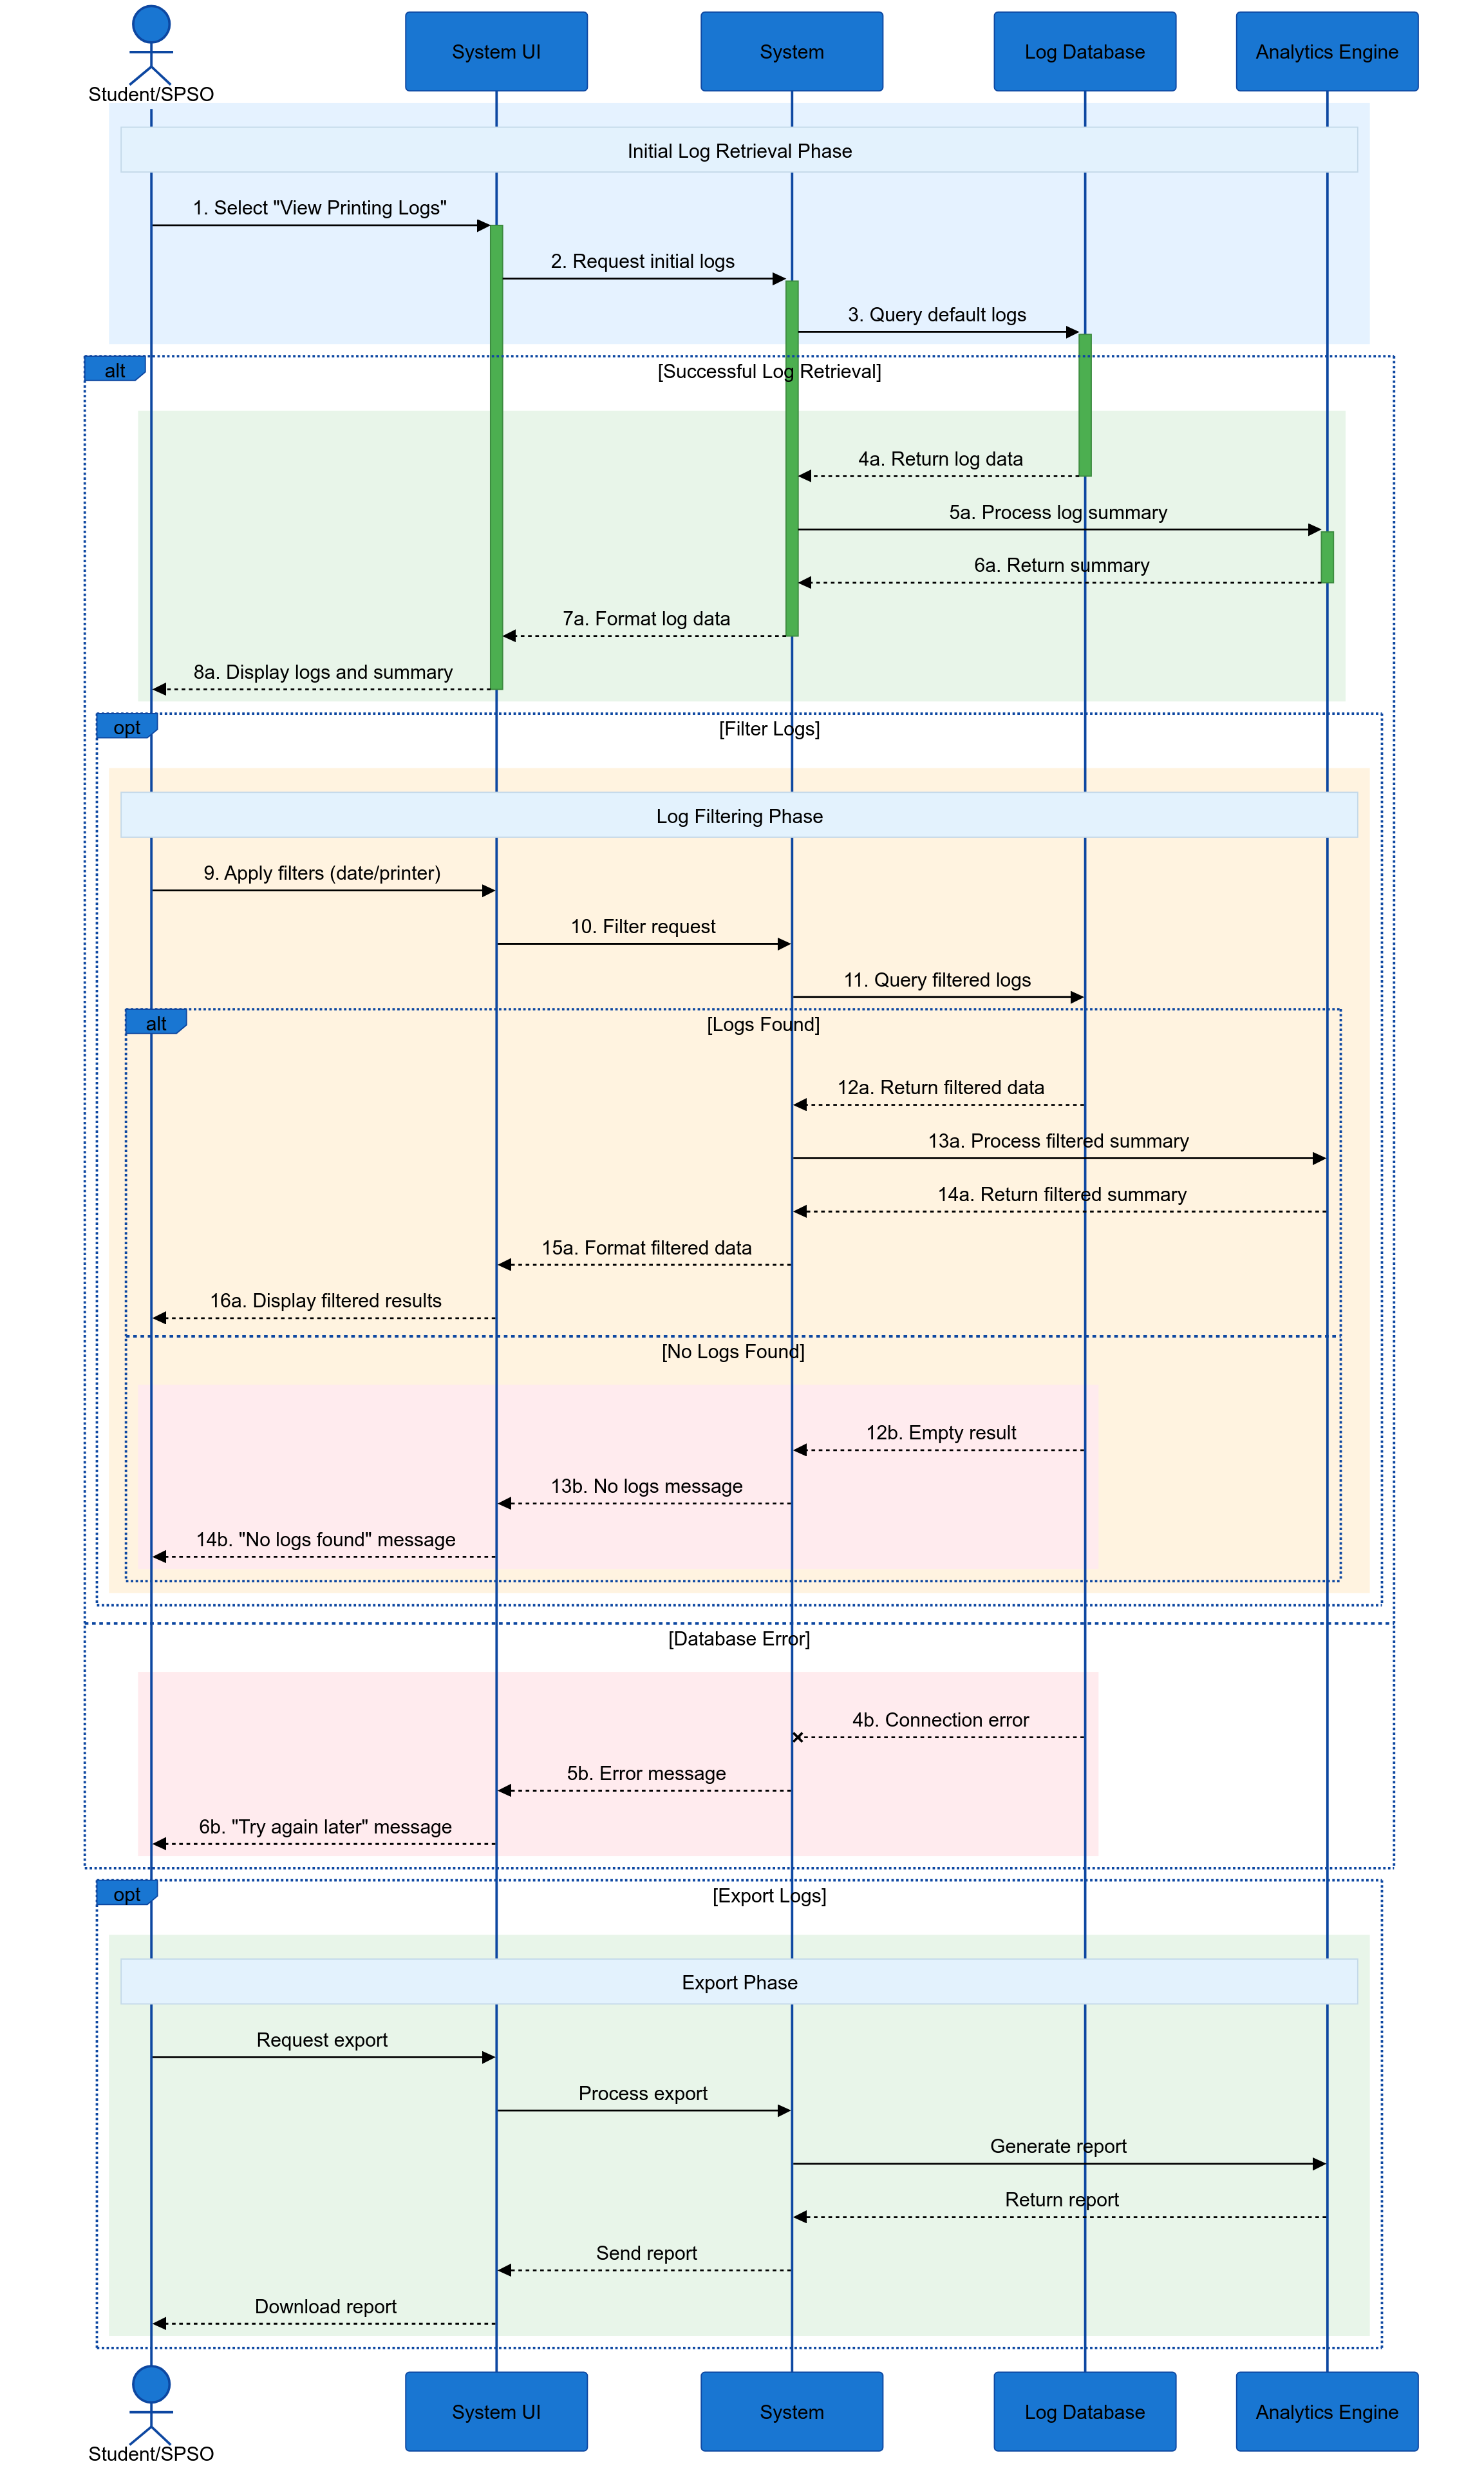
\includegraphics[width=0.85\textwidth]{sequence_diagram/View Printing Logs.png}
    \caption{UseCase - View Priting Logs}
    \label{fig:view_printing_logs}
    
\end{figure}

This diagram (Figure \ref{fig:view_printing_logs}) represents a use case for viewing printing logs in a system. It begins with a "Student/SPSO" selecting the "View Printing Logs" option. The system then initiates a request to retrieve initial logs, querying the default logs from the log database. If log retrieval is successful, the log data is returned, and a log summary is processed by the analytics engine, followed by the formatted log data and summary being displayed. The user has the option to apply filters such as date or printer, which triggers another query to retrieve filtered logs. If logs are found, the system returns the filtered data and displays it; otherwise, a "No logs found" message is shown. In case of a database error, an error message is shown with a suggestion to "try again later." Additionally, the user can request to export the logs, which prompts the system to process and generate a report for download. This sequence ensures comprehensive interaction flows for log viewing, filtering, error handling, and export functionalities.

\section{Class Diagram}
\newpage
\thispagestyle{empty}
\begin{landscape} % Start landscape mode
    
    \begin{figure}[H]
        \centering
        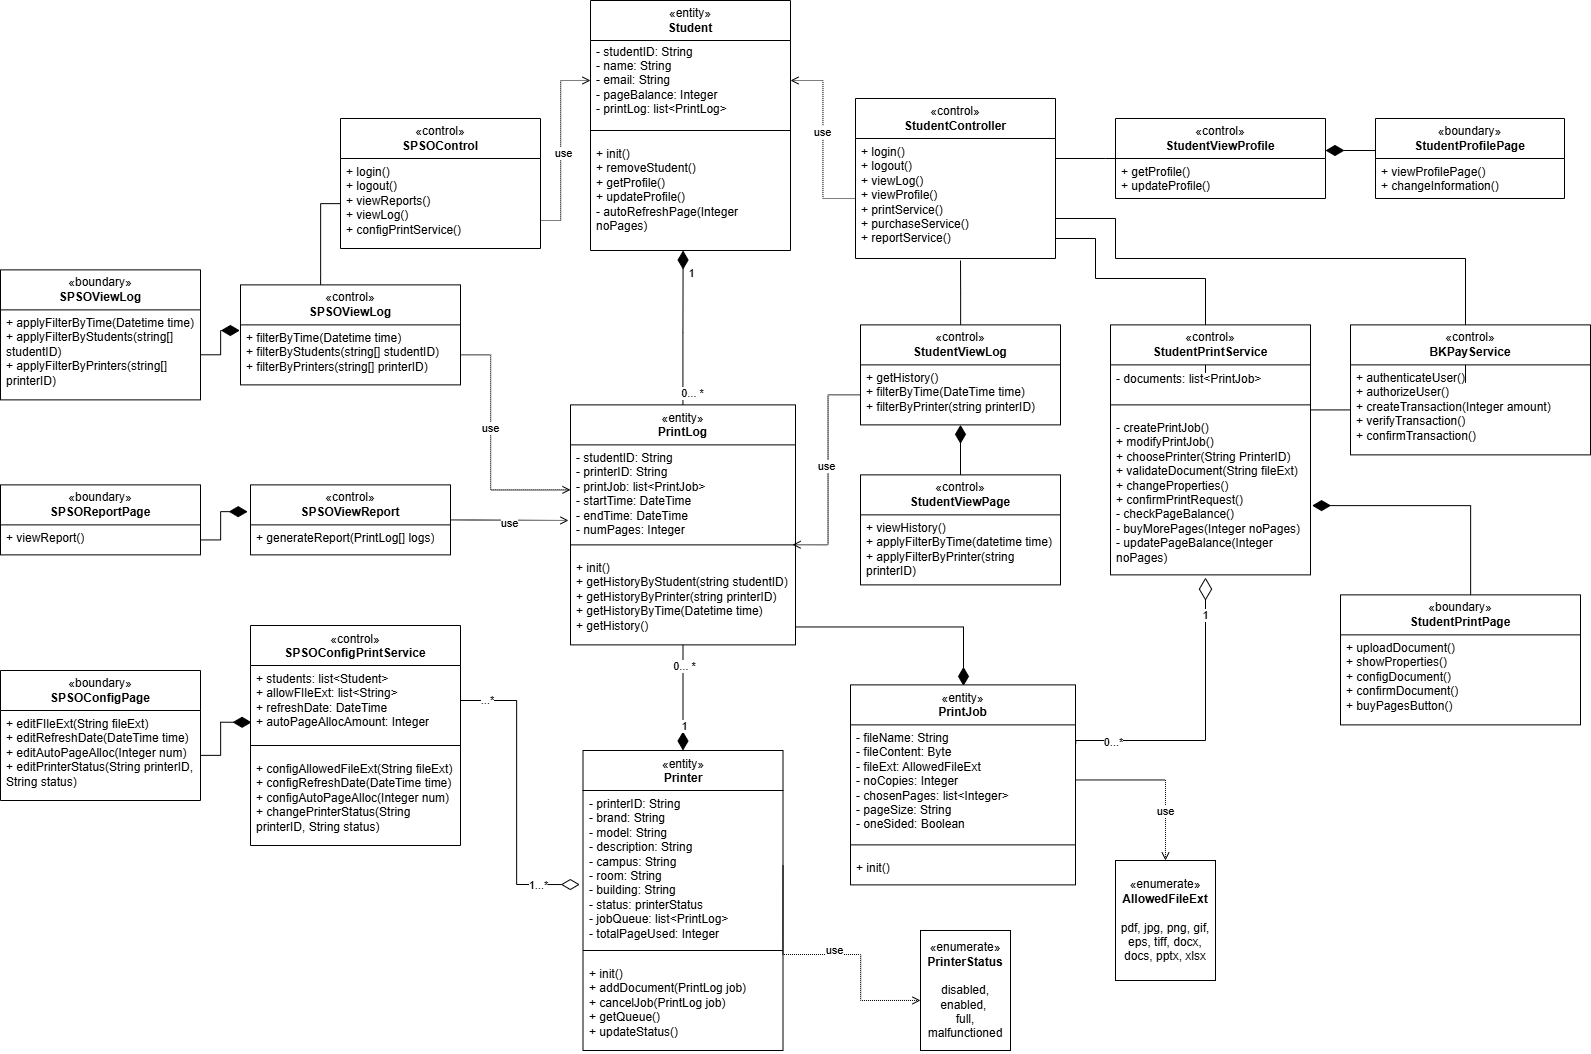
\includegraphics[width=1.3\textwidth]{class_diagram.png}
            \caption{Class Diagram}
        \label{fig:class_diagram}
    \end{figure}    
    
\end{landscape} % End landscape mode

\newpage
\section{Development MVP 1}

\begin{figure}[H]
    \centering
    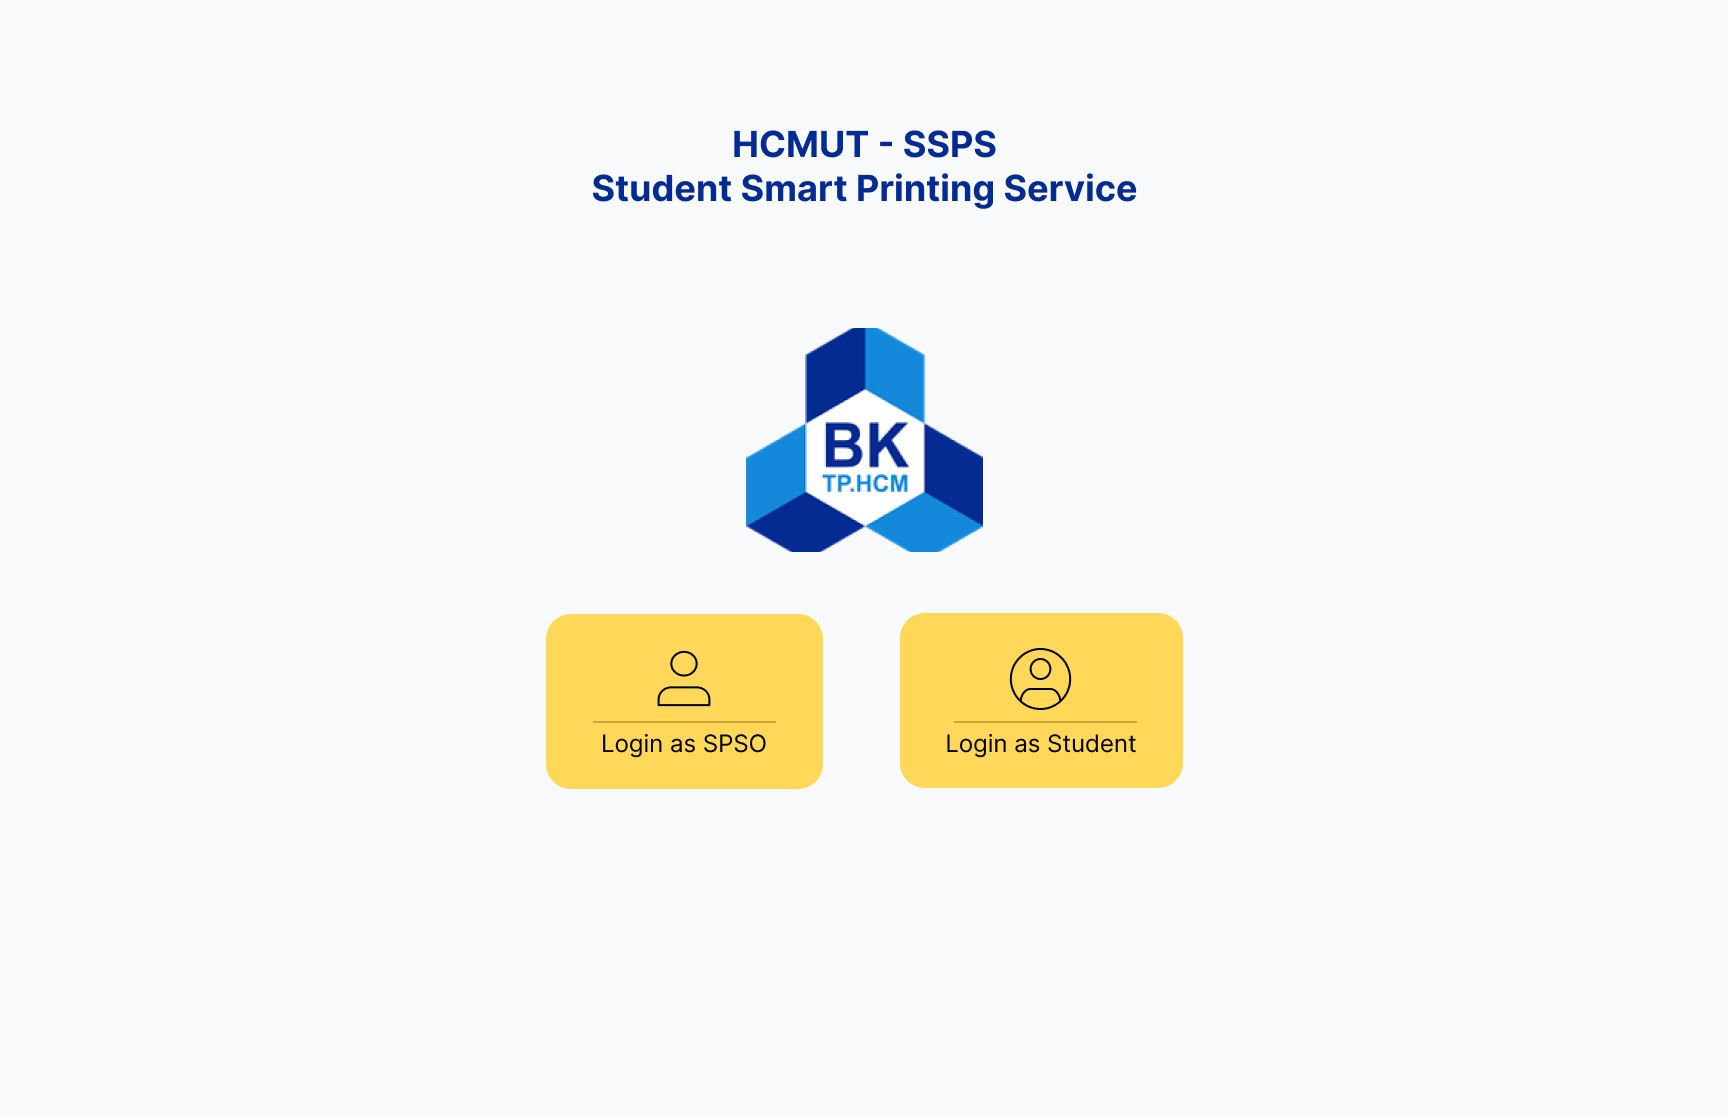
\includegraphics[width = 1\textwidth, ]{images/UI/Login Page.png}
    \caption{Login Page}
\end{figure}  

\begin{figure}[H]
    \centering
    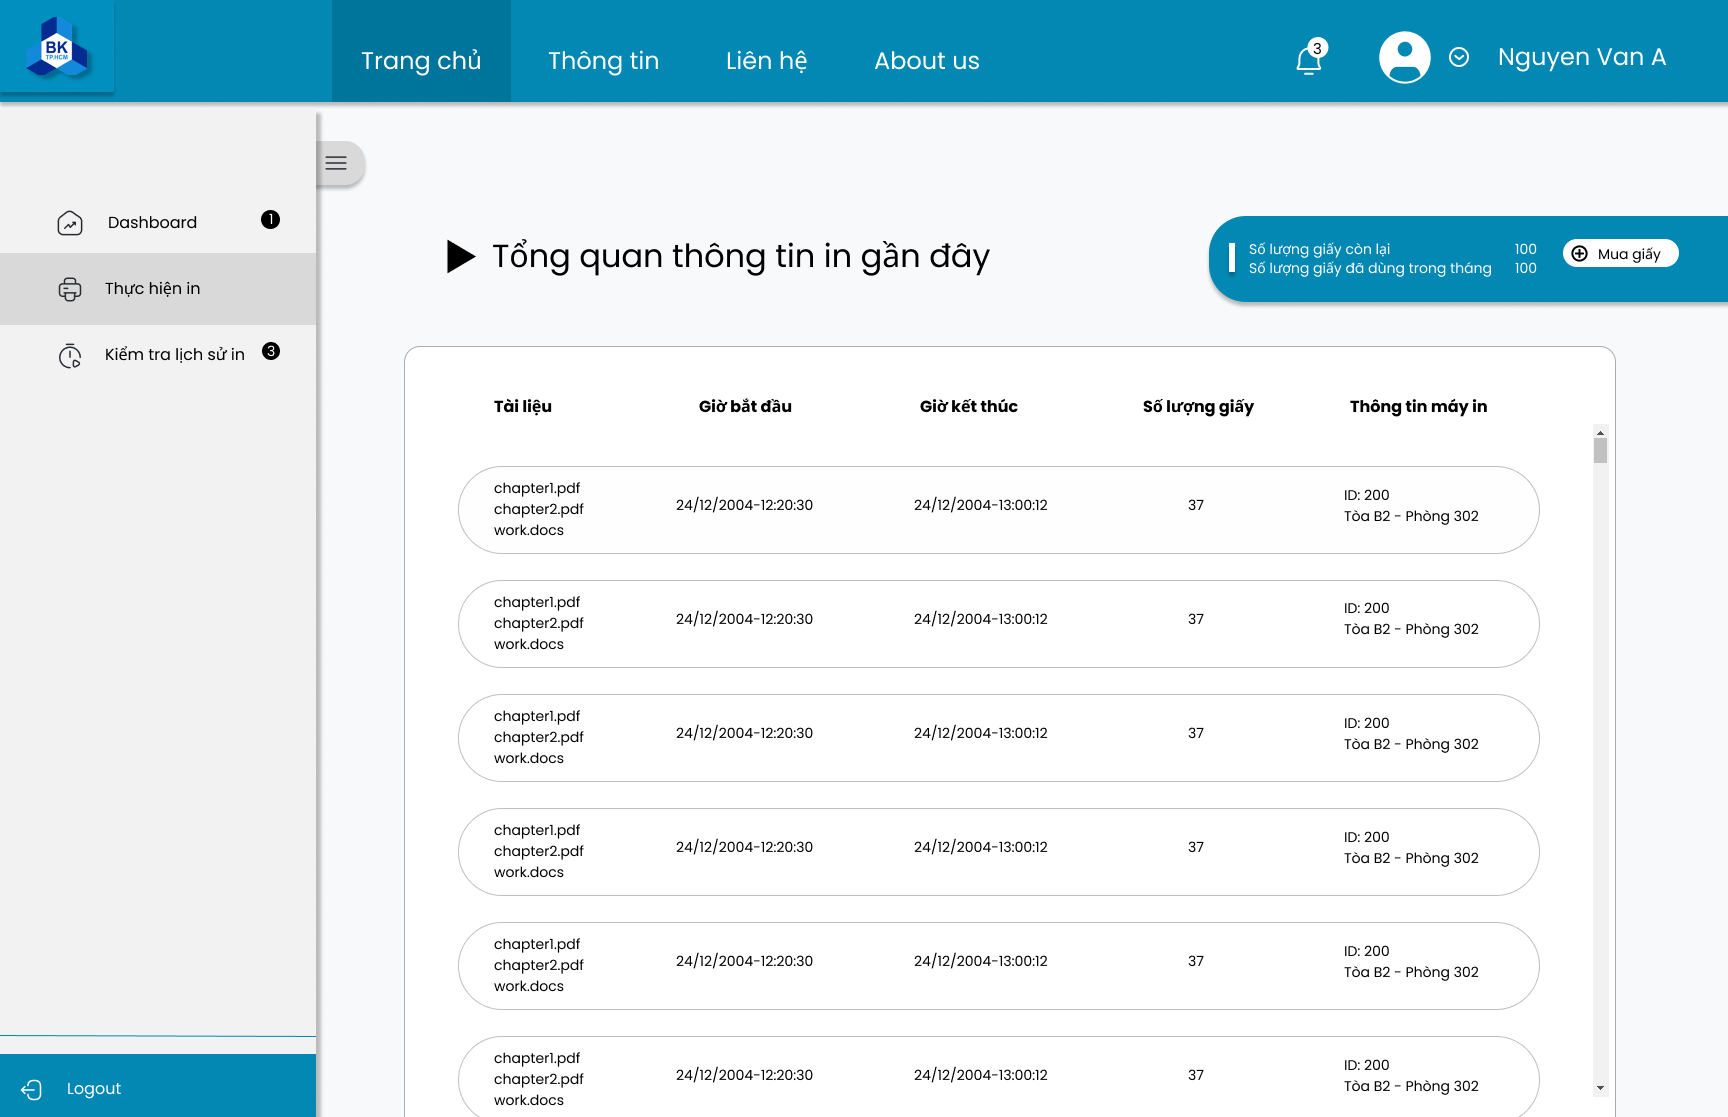
\includegraphics[width = 1\textwidth, ]{images/UI/Bảng điều khiển sinh viên.png}
    \caption{Student Dashboard Page}
\end{figure}  

\begin{figure}[H]
    \centering
    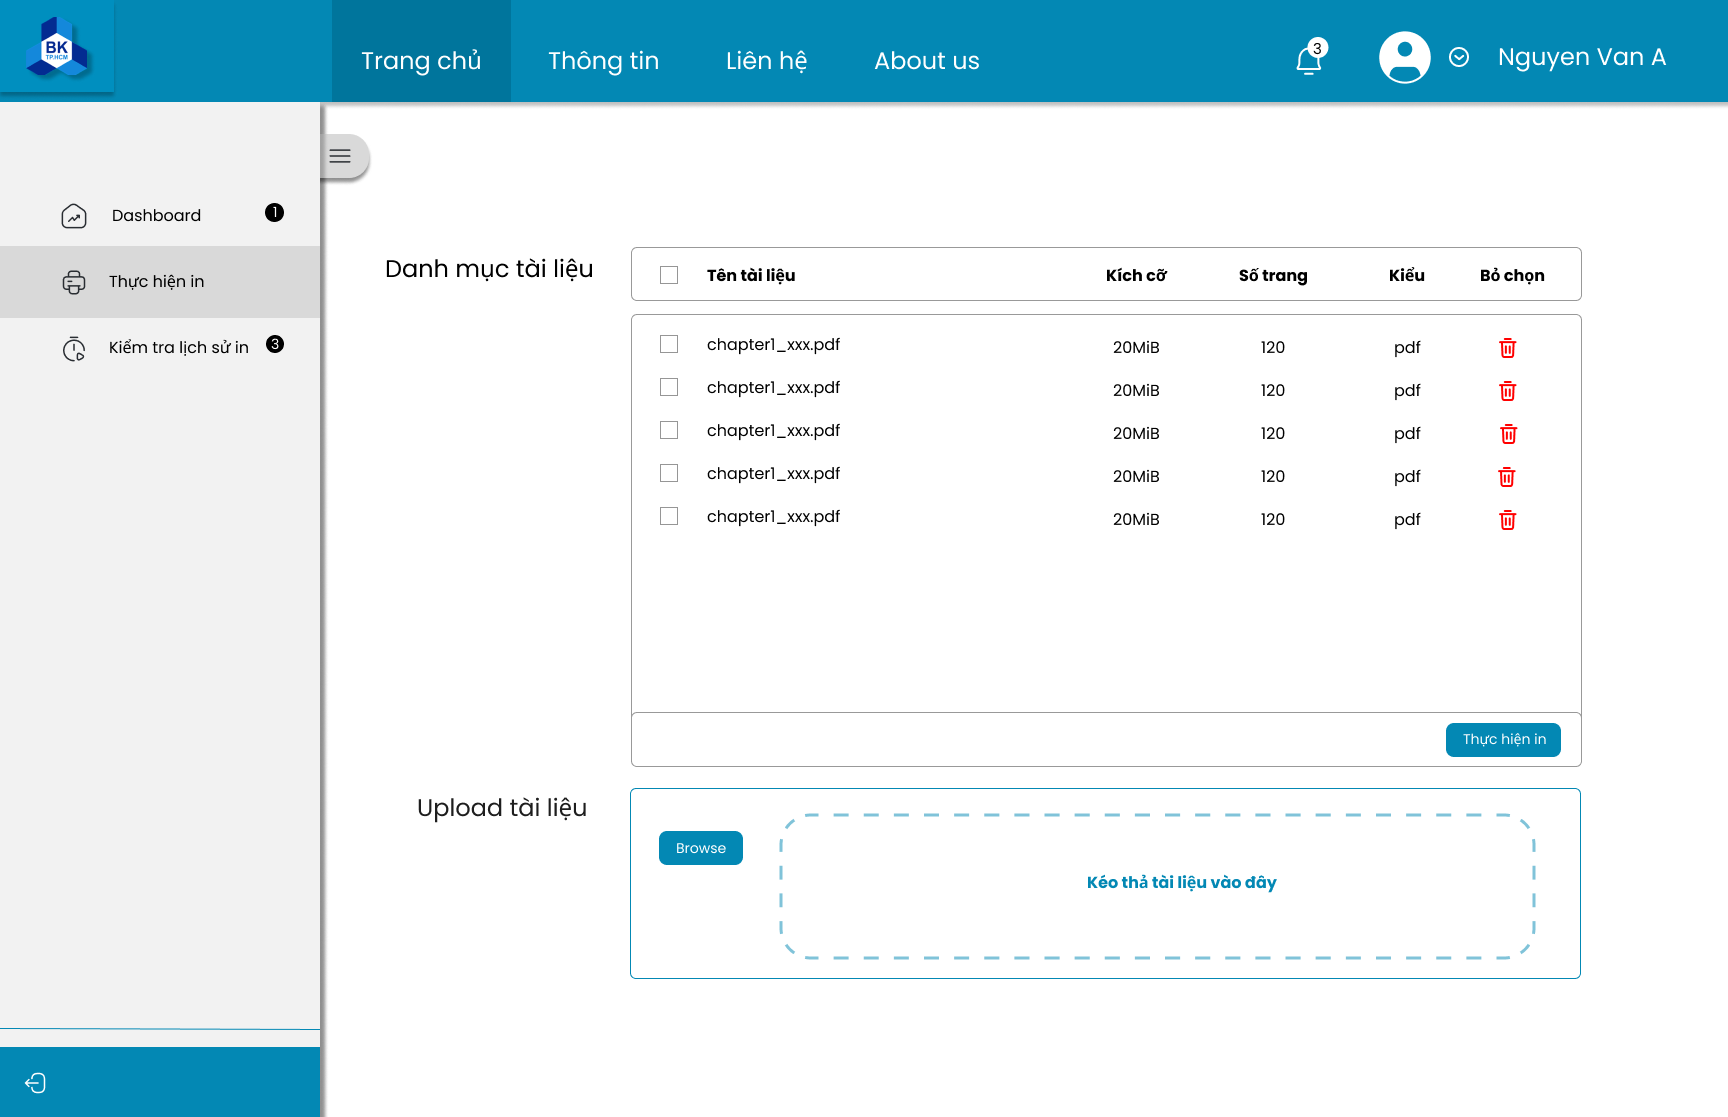
\includegraphics[width = \textwidth, ]{images/UI/Bảng in sinh viên.png}
    \caption{Student Printing Page}
\end{figure}  

\begin{figure}[H]
    \centering
    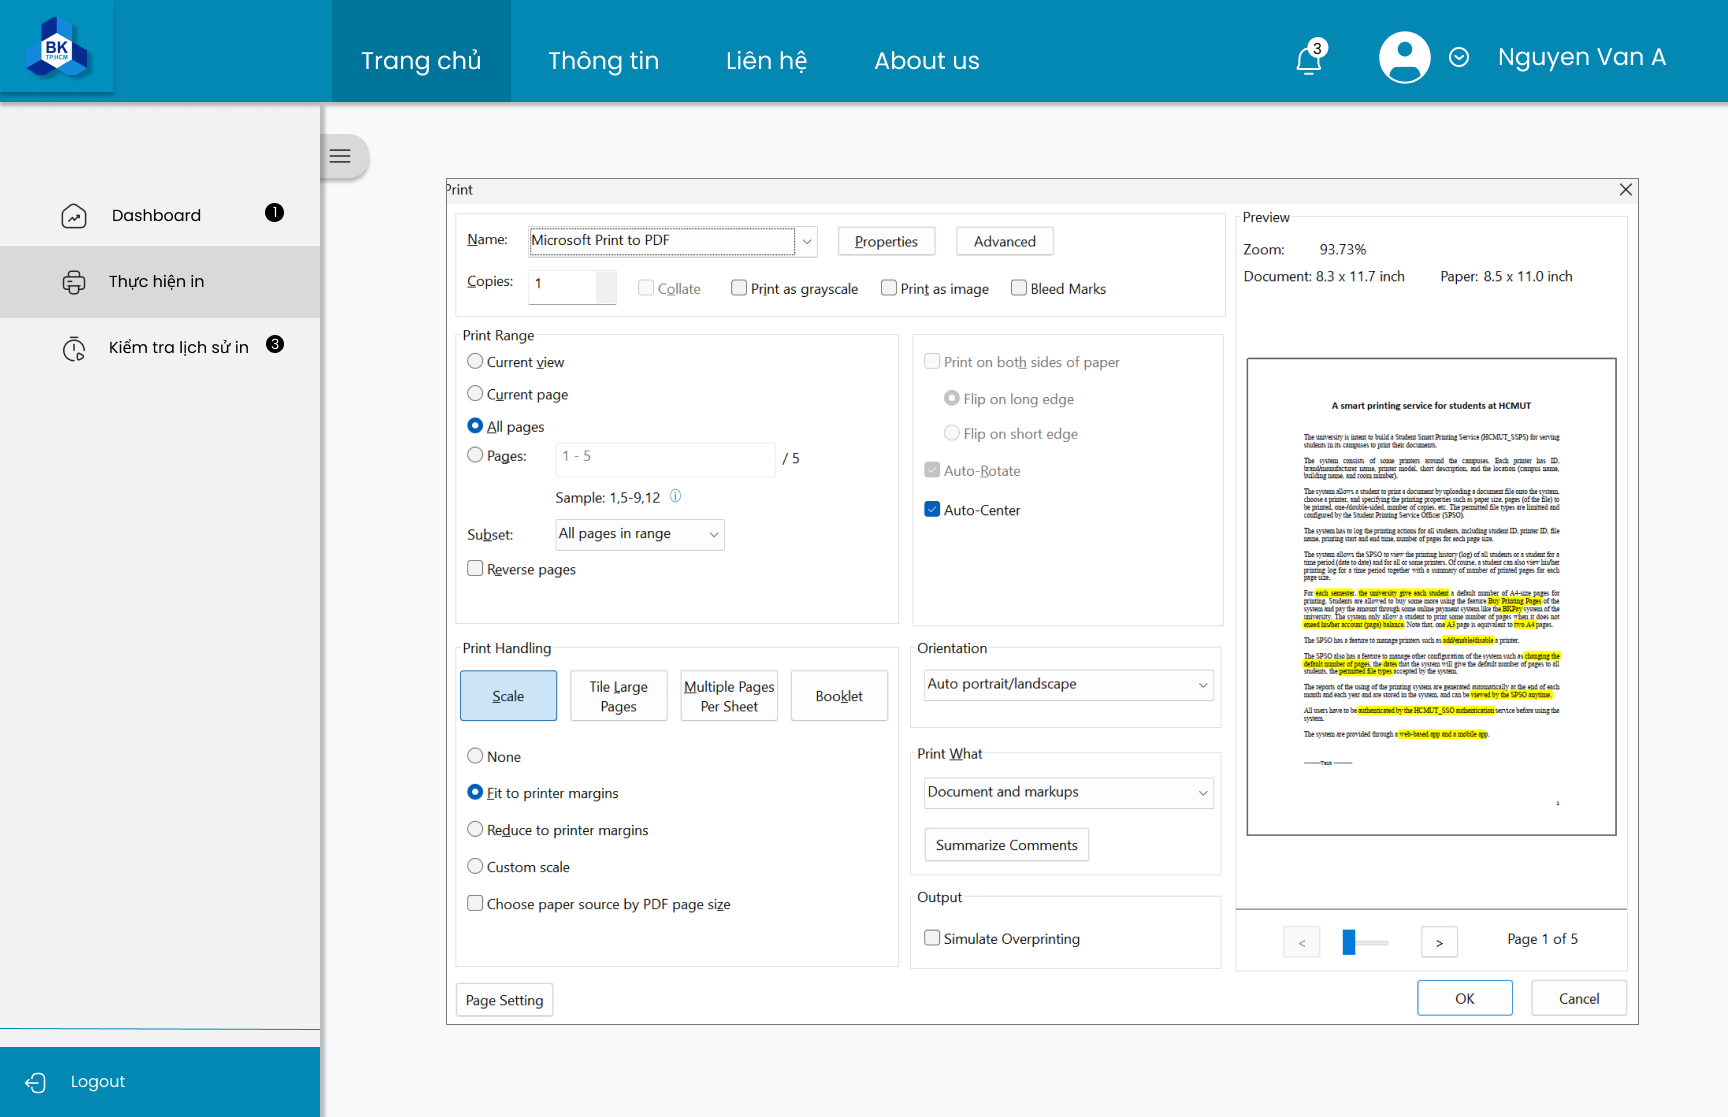
\includegraphics[width = \textwidth, ]{images/UI/Bảng in sinh viên 2.png}
    \caption{Student Printing Configuration Dialog}
\end{figure}  

\begin{figure}[H]
    \centering
    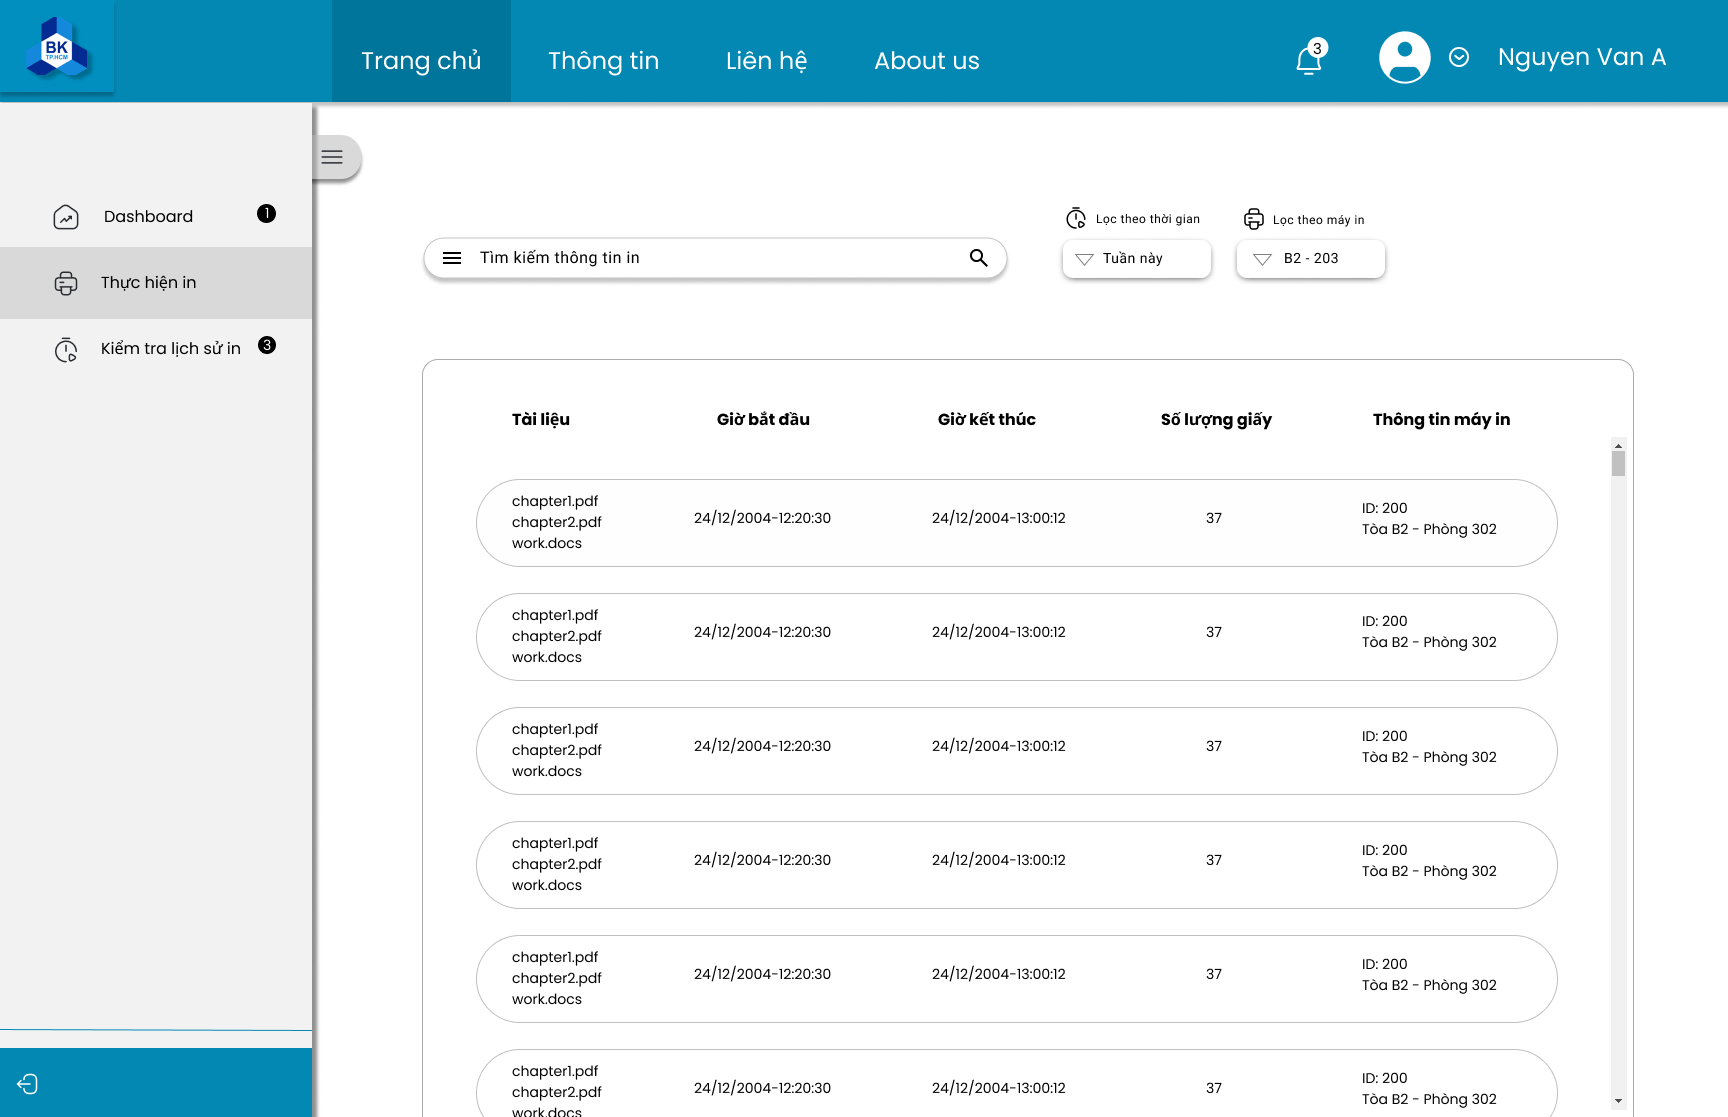
\includegraphics[width = \textwidth, ]{images/UI/Tra lịch sử sinh viên.png}
    \caption{Student History Log}
\end{figure}  

\begin{figure}[H]
    \centering
    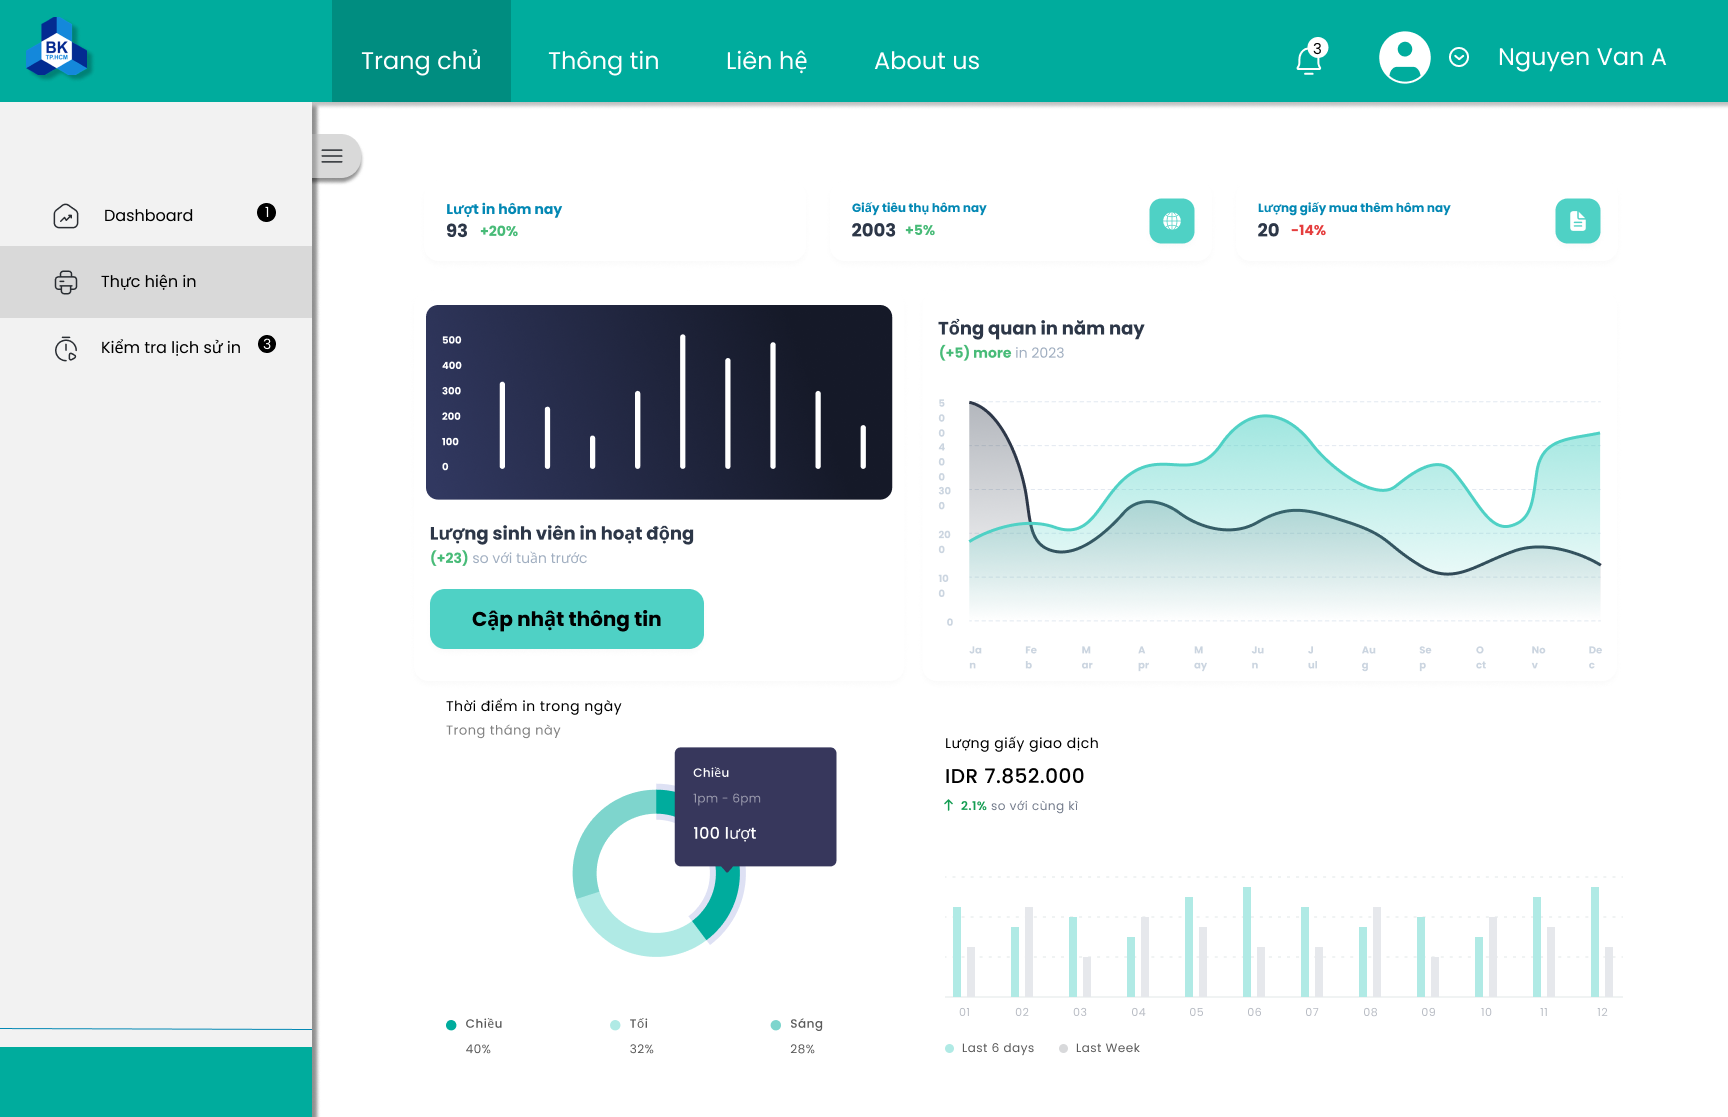
\includegraphics[width = \textwidth, ]{images/UI/Bảng điều khiển SPSO.png}
    \caption{SPSO Dashboard}
\end{figure}  

\begin{figure}[H]
    \centering
    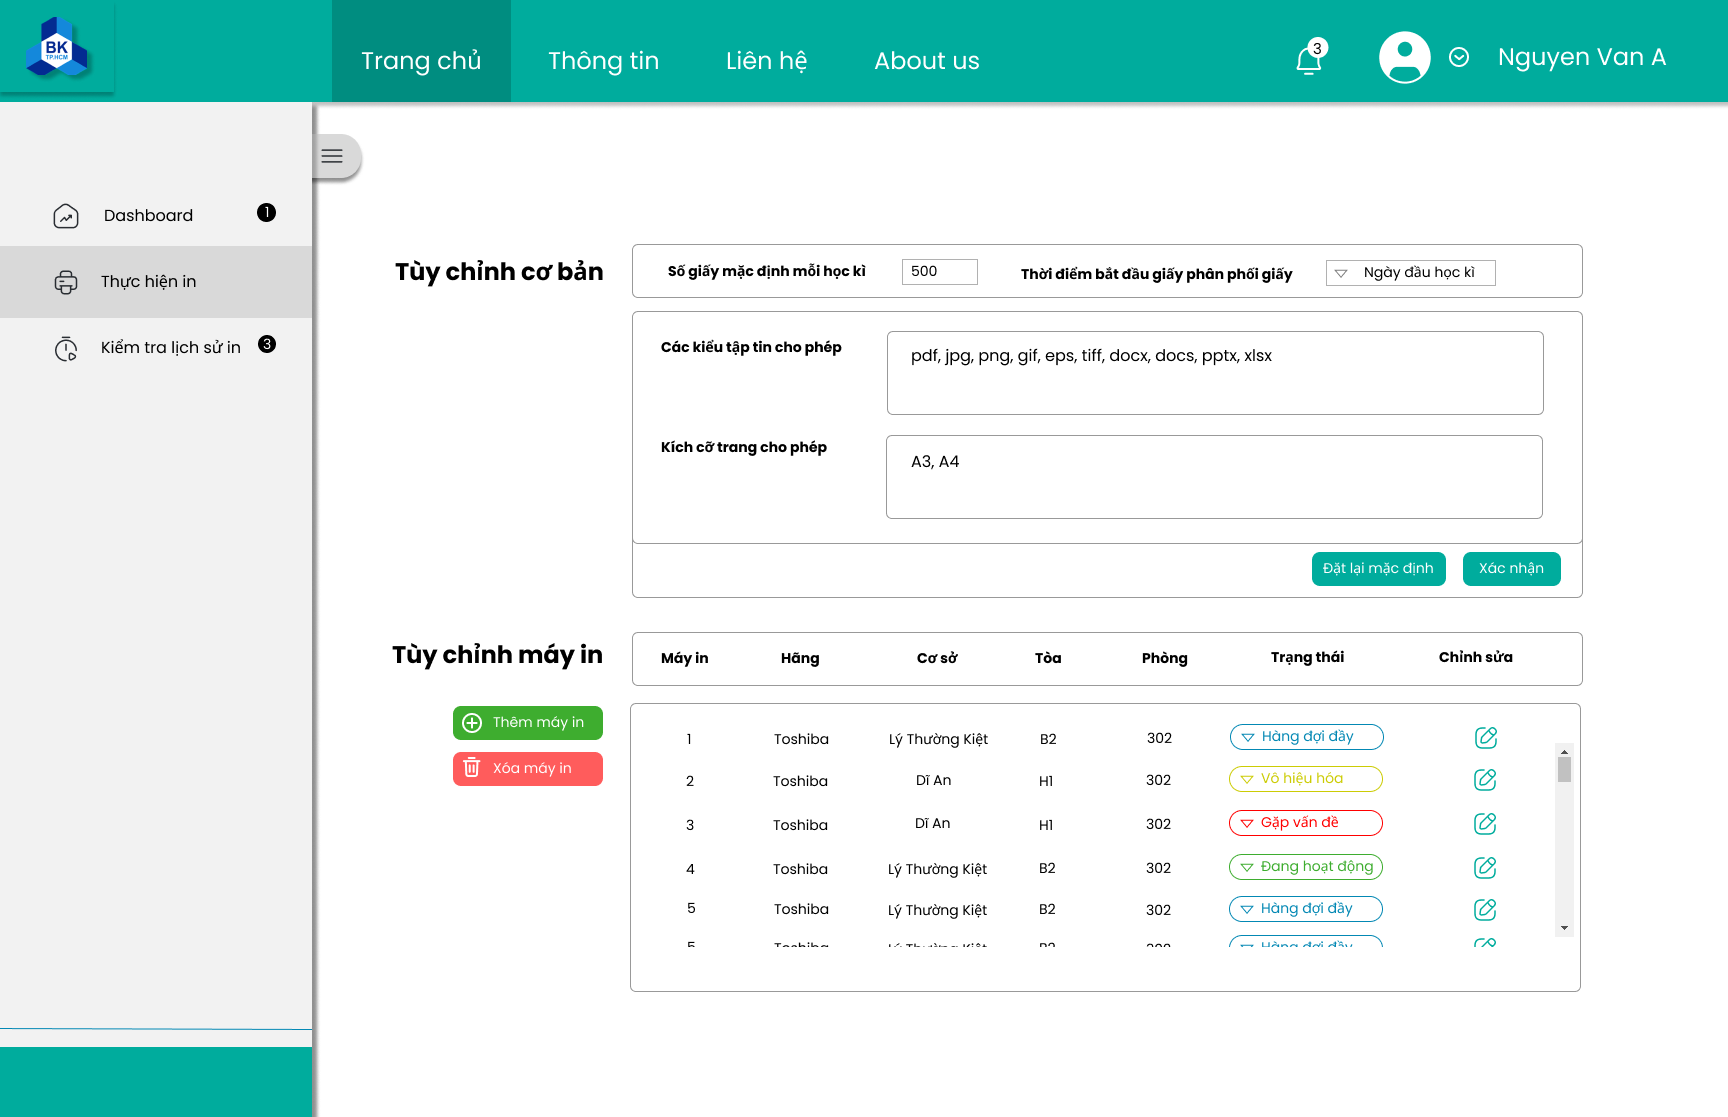
\includegraphics[width = \textwidth, ]{images/UI/Thay đổi in SPSO.png}
    \caption{SPSO Printing Configuration}
\end{figure}  

\begin{figure}[H]
    \centering
    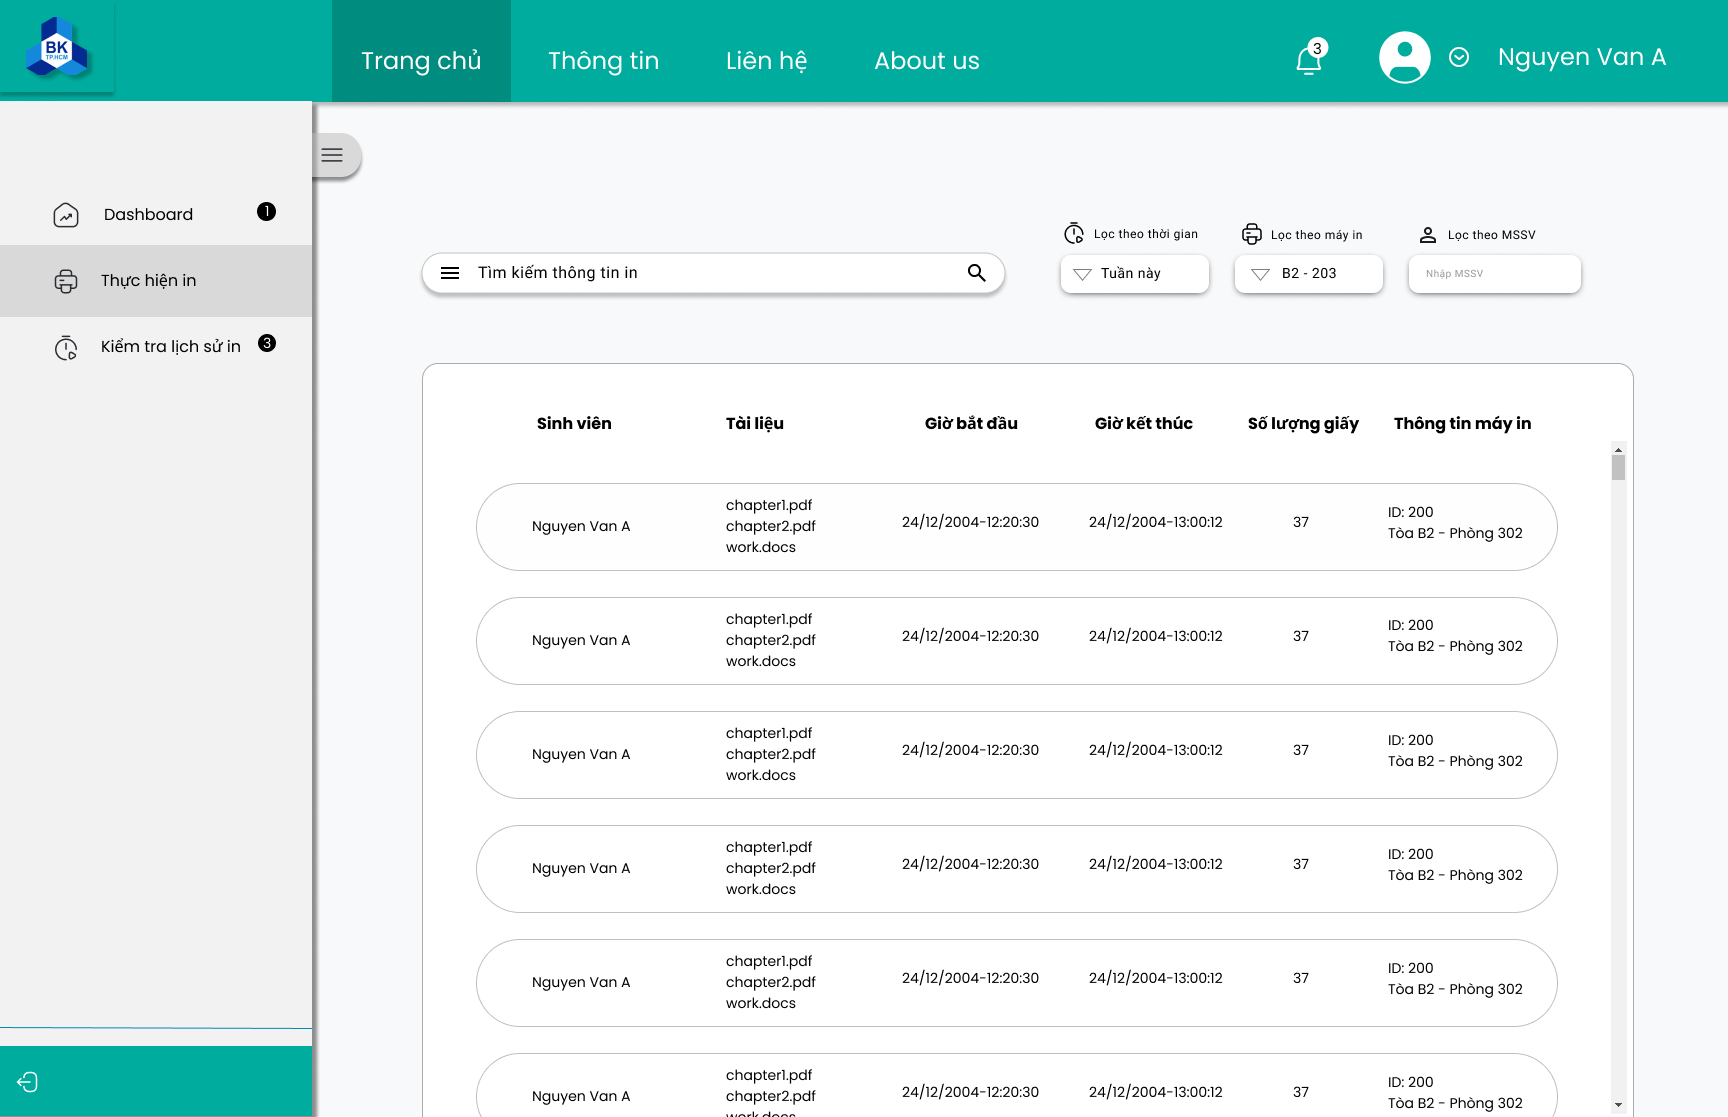
\includegraphics[width = \textwidth, ]{images/UI/Tra lịch sử SPSO.png}
    \caption{SPSO History Log}
\end{figure}  



\href{}{Link Figma}

\newpage
\chapter{Architecture Design}

\section{Architectural Diagram}

\begin{figure}[H]
    \centering
    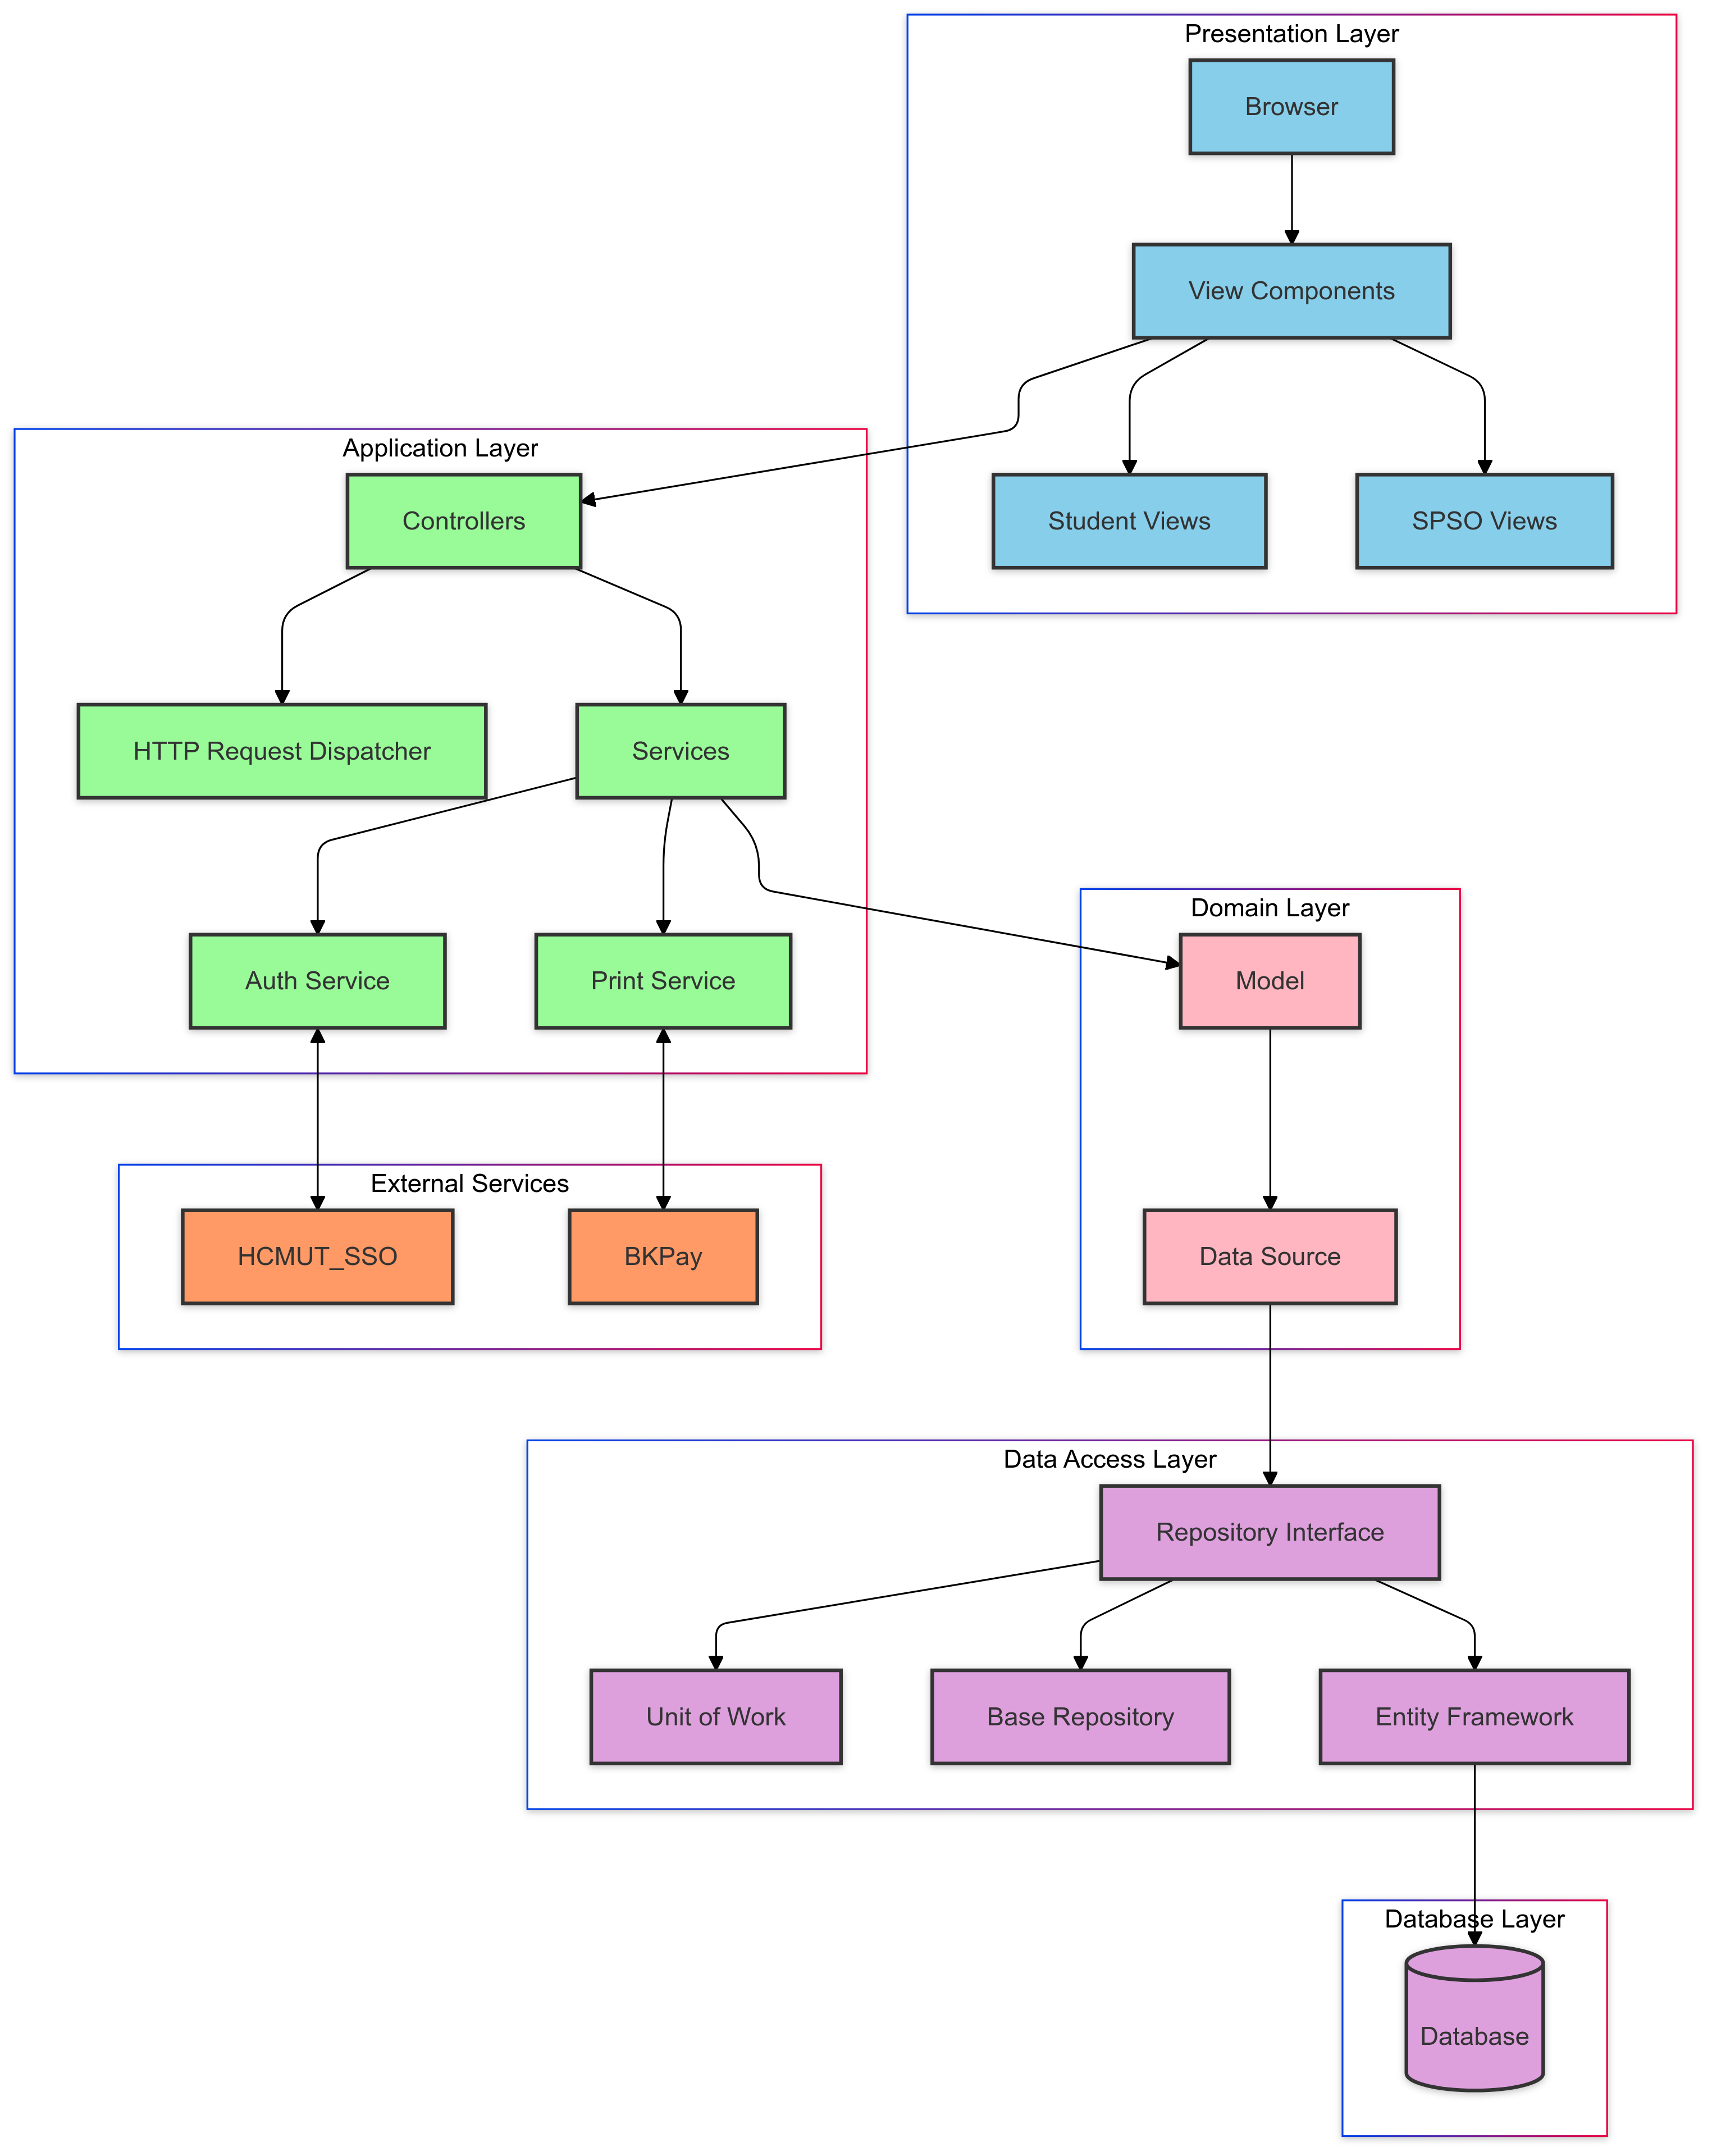
\includegraphics[width=0.78\linewidth]{images/architectural_diagram.png}
    \caption{Architectural Diagram}
    \label{fig:enter-label}
\end{figure}

\subsection{Presentation Strategy} 

The HCMUT-SSPS system implements a client-side architecture focusing on separation of concerns between UI components and business logic. We adopt a component-based architecture to promote reusability and maintainability across different views (student and SPSO interfaces). The presentation layer implements the Observer pattern for state management, ensuring consistent data flow and real-time updates for printing statuses. For optimal performance, we utilize lazy loading for resource-heavy components and implement efficient client-side caching mechanisms. The UI follows a responsive design approach with mobile-first principles, ensuring accessibility across different devices and screen sizes.

\subsection{Data Storage Approach} 

Our data persistence strategy implements a layered approach with clear separation between data access and business logic. The system utilizes a relational database for structured data (user profiles, transactions, print logs) with a document store for handling print job files and documents. We implement the Repository pattern to abstract data access operations, coupled with Unit of Work pattern for maintaining data consistency across transactions. The storage layer includes caching mechanisms for frequently accessed data and implements database sharding for horizontal scalability. This architecture supports our requirements for data integrity, performance, and scalability while maintaining ACID compliance for critical transactions.

\subsection{API Management} 

The API architecture follows RESTful principles with clear resource-oriented endpoints and standardized response formats. We implement an API Gateway pattern for request routing, composition, and protocol translation. Authentication is integrated with HCMUT's SSO system, while authorization implements role-based access control (RBAC). The API layer includes the following;

\begin{multicols}{2}    
\begin{itemize}
    \item Request validation and sanitization
    \item Rate limiting and throttling
    \item Standardized error handling
    \item API versioning through URL paths
    \item Response compression and caching
    \item Monitoring and logging capabilities
\end{itemize}
\end{multicols}

\subsection{Key Architectural Principles}

\subsubsection{Separation of Concerns}
\begin{itemize}
    \item Clear boundaries between presentation, business logic, and data access
    \item Modular components for easy maintenance and testing
    \item Standardized interfaces between layers
\end{itemize}

\begin{multicols}{2}
\subsubsection{Scalability}
\begin{itemize}
    \item Horizontal scaling capabilities
    \item Efficient caching strategies
    \item Load balancing support
\end{itemize}

\subsubsection{Security}
\begin{itemize}
    \item Integration with institutional SSO
    \item Secure data transmission
    \item Input validation and sanitization
    \item Access control and audit logging
\end{itemize}

\subsubsection{Maintainability}
\begin{itemize}
    \item Documented API contracts
    \item Clear coding standards
    \item Version control strategies
    \item Comprehensive logging
\end{itemize}

\subsubsection{Performance}
\begin{itemize}
    \item Optimized database queries
    \item Client-side caching
    \item Resource optimization
    \item Response compression
\end{itemize}
\end{multicols}

\newpage
\section{Component Diagram}
\subsection{Component Diagram Design}
\begin{figure}[H]
    \centering
    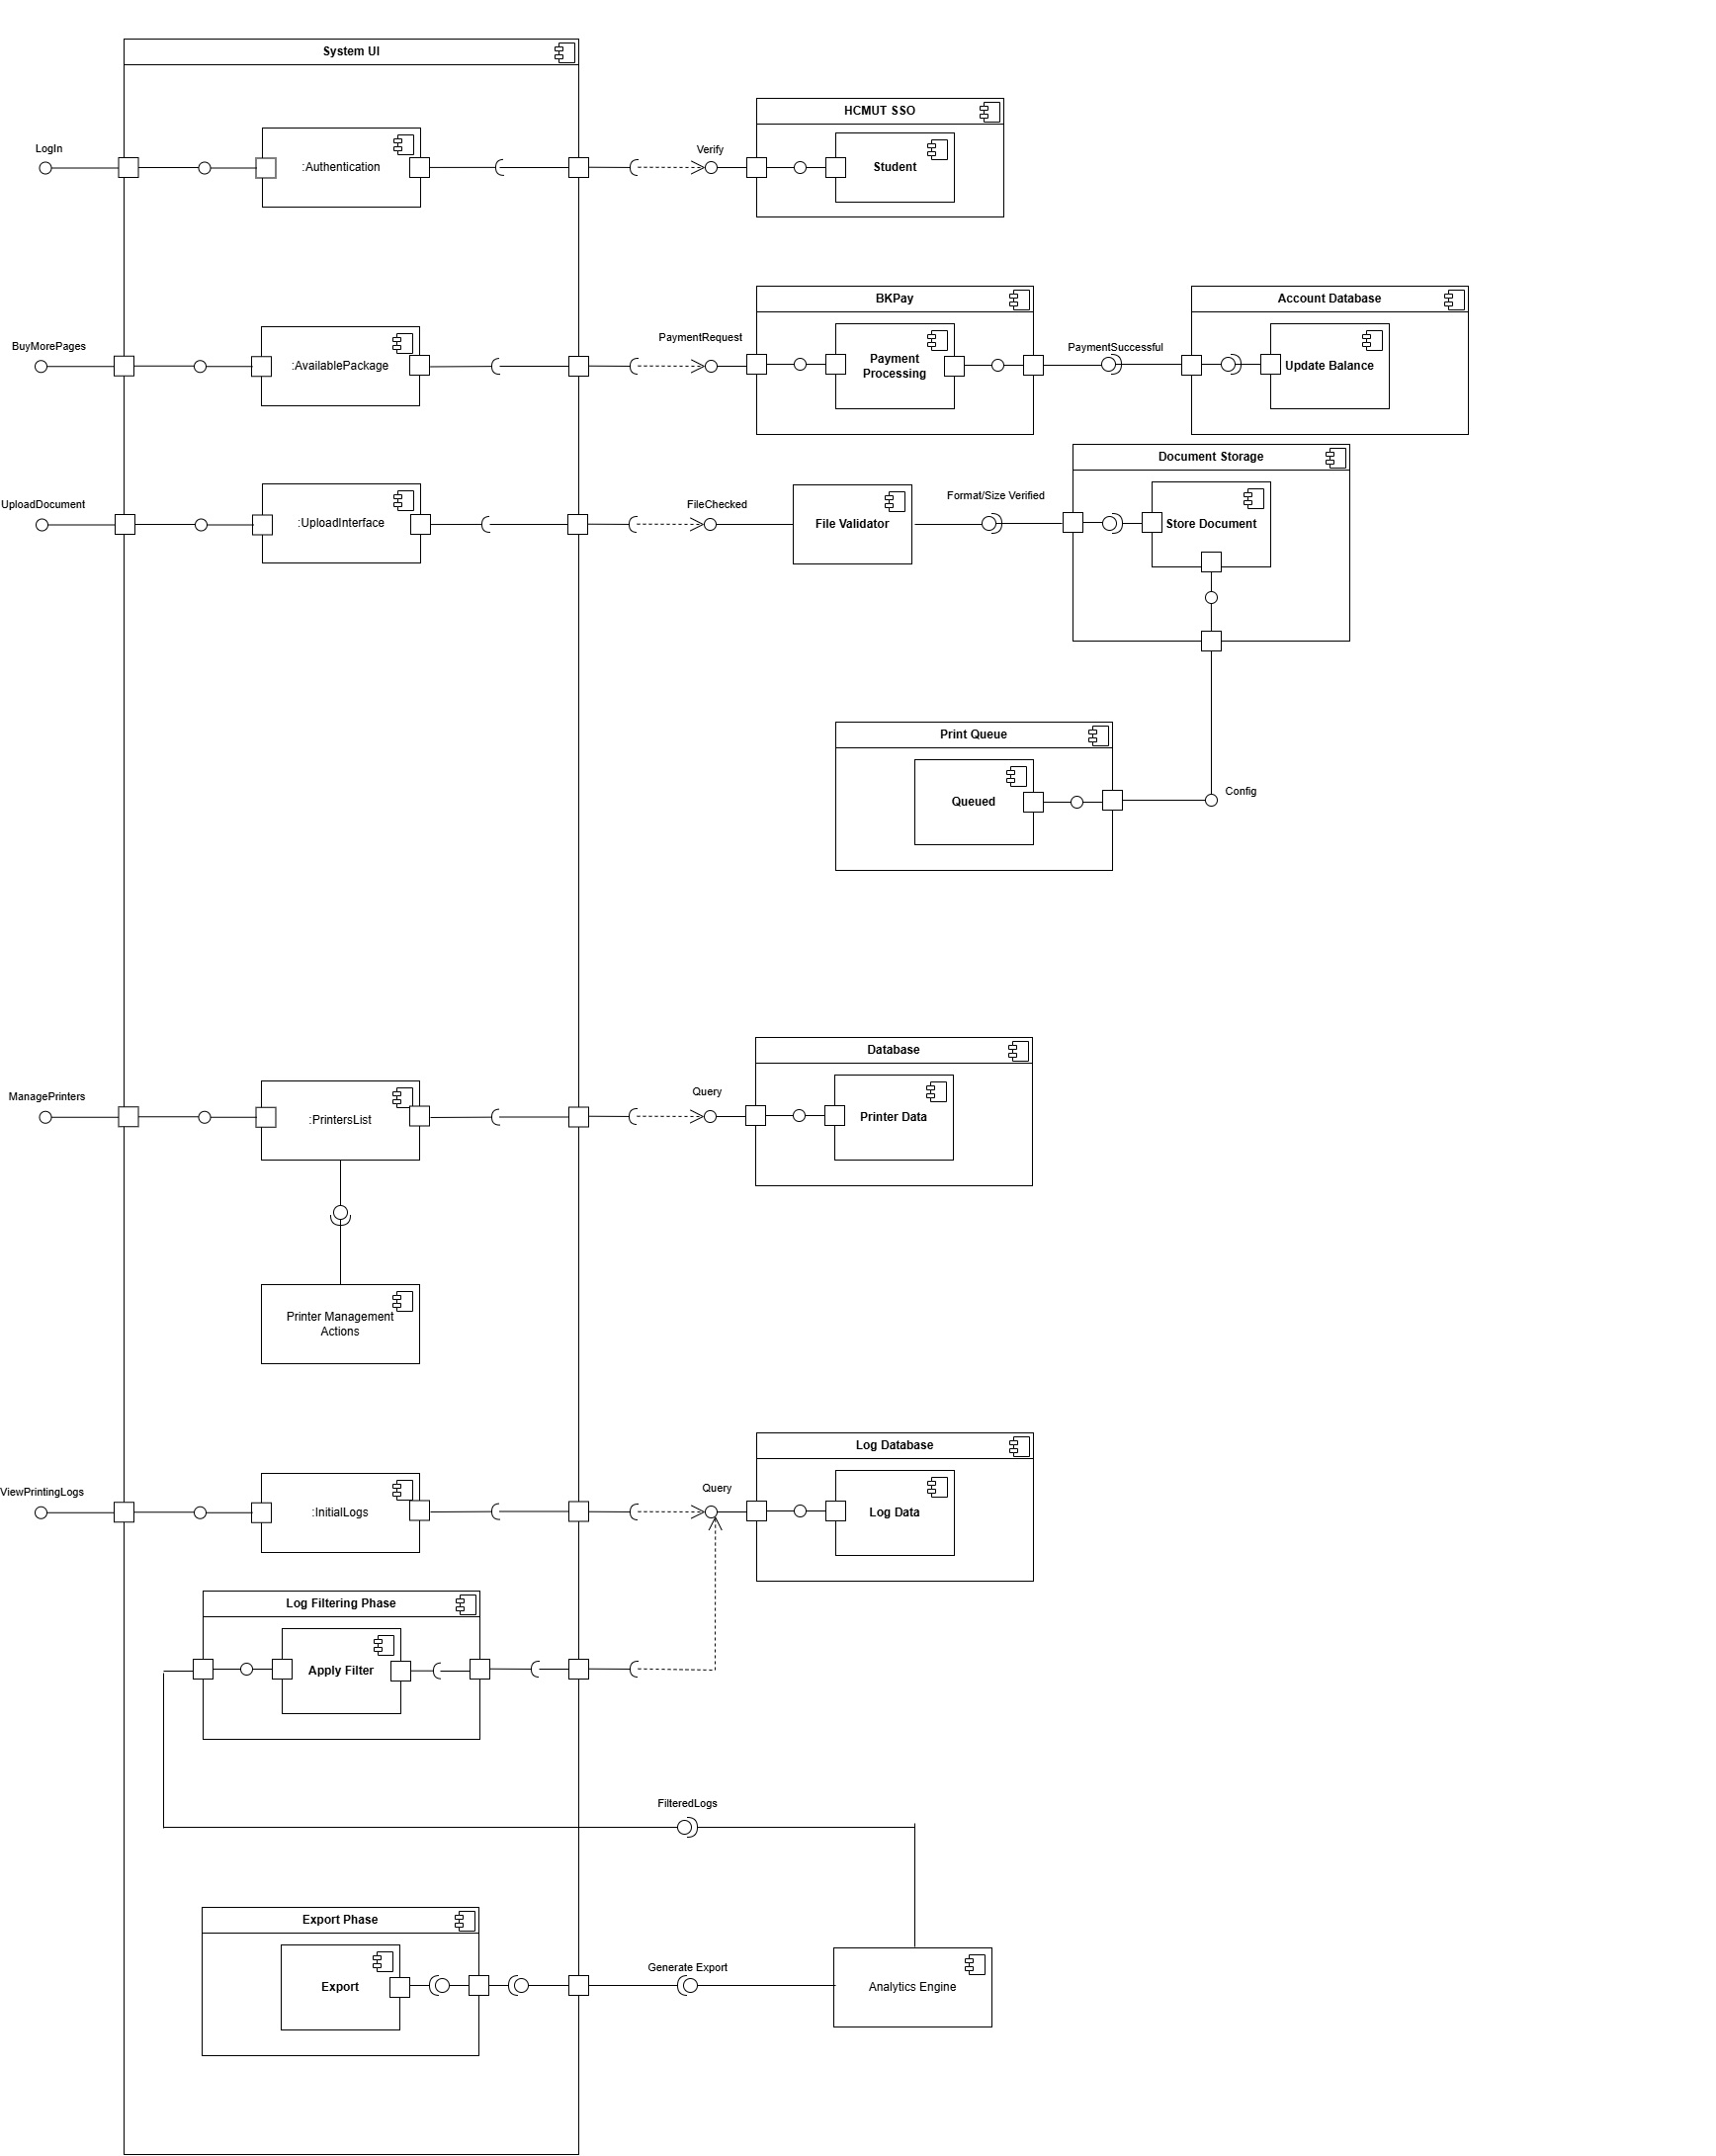
\includegraphics[width=1\linewidth]{images/component_diagram.png}
    \caption{Component Diagram}
    \label{fig:enter-label}
\end{figure}

\newpage
\subsection{Description}
The component diagram highlights the major components and their interactions with each other to fulfill the system’s functionality.
\begin{enumerate}
    \item  The “LogIn” diagram handles user authentication which interacts with the “HCMUT SSO” to verify user credentials and the System UI to provide a user interface for login.
    \item The “BuyMorePages” diagram give user choice of package to buy, which interacts with “BKPay” for Students to pay for the chosen and the System UI to provide a user interface for the service. The “Account Database” will interact with the “BKPay” as long as the payment is successful.
    \item The “UploadDocument” diagram interacts with the System UI to provide a user interface to upload the user document and interacts with the “File Validator” to have the file’s format and size checked. Since the uploaded files meet the required specifications, they are stored in the Document Storage and also queued for printing after print setting configuration.
    \item The “ManagePrinters” diagram provide the user interface where users can view and manage printers. The PrinterList queries the “Database” to manage printers and printers data. The “Printers Management Actions” start its implementation when users perform printers management actions, querying “Database” for printers data.
    \item The “ViewPrintingLogs” diagram provides the user interface where users can view and interact with the logs, the System querying the “Log Database” for the log data. After user applying specific filter. The “Log Filtering Phase” queries the “Log Database” for the requested filtered data and show them for users. In the “Export Phase”, the system processes the user’s request and generates a report through the Analytics Engine, the engine get the filtered logs data from the “Log Filtered Phase”. The generated report is then made available for users to download.
\end{enumerate}

\chapter{Implementation - Sprint 1}
\section{Usability Test}
We have taken an Usability Test using a group of 5 users. The Usability Test is divided into two sections included (SPSS for Student and SPSS for SPSO). For each section, we want to have feedbacks of participants for the UI of the system and research their experience by using multiple choice questions. We use figma prototype as an object to experience. The link of figma prototype has been provided above.
\subsection{SPSS for Student}
\begin{enumerate}
    \item \textbf{LOGIN PAGE} \\
    In this question, we research the behavior of participants in using LOGIN PAGE.
\begin{figure}[!h]
    \centering
    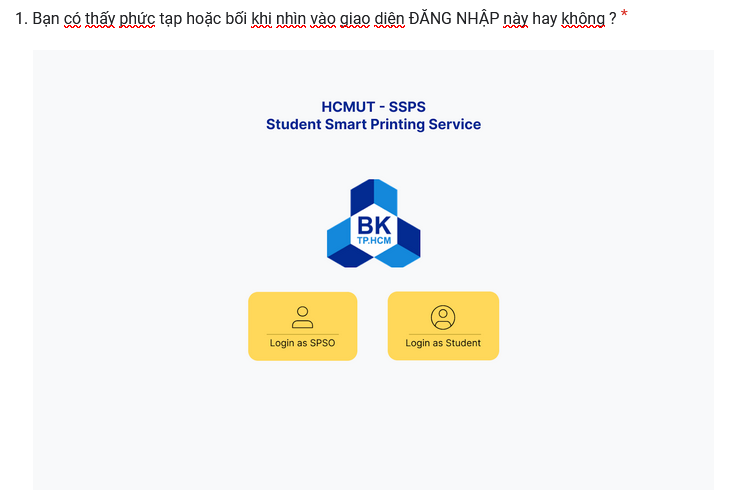
\includegraphics[width=0.8\linewidth]{images/image_uasbility/Q1_Stu.png}
    \caption{LOGIN PAGE}
    \label{fig:LOGIN PAGE}
\end{figure}
\newpage
According to the survey, there are 40\% of participants find it a little curious to understand this task.
\begin{figure}[!h]
    \centering
    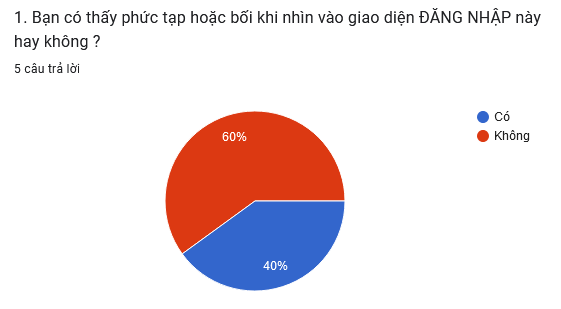
\includegraphics[width=0.8\linewidth]{images/image_uasbility/A1_Stu.png}
    \caption{Char illustrates the result of Question 1}
    \label{fig:Chat illustrates the results of Question 1}
\end{figure}

    \item \textbf{DASHBOARD PAGE} \\
    In this Question, we research the behavior of participants in using DASHBOARD PAGE.
\begin{figure}[!h]
    \centering
    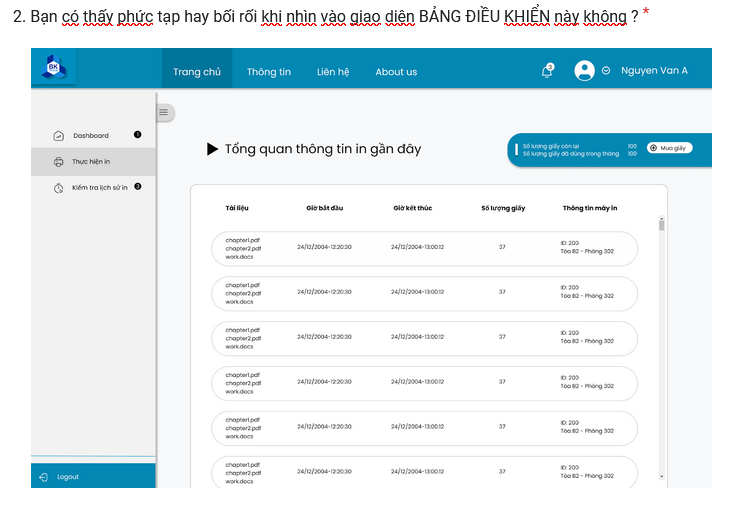
\includegraphics[width=0.8\linewidth]{images/image_uasbility/Q2_Stu.png}
    \caption{DASHBOARD PAGE}
    \label{fig:DASHBOARD}
\end{figure}
\newpage
According to the survey, there are 40\% of participants find it a little curious to understand this task.
\begin{figure}[!h]
    \centering
    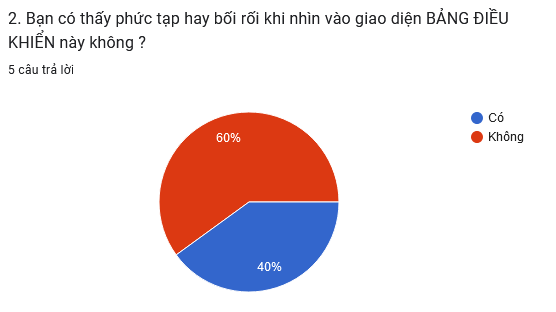
\includegraphics[width=0.8\linewidth]{images/image_uasbility/A2_Stu.png}
    \caption{Chart illustrates the result of Question 2}
    \label{fig:Chart illustrates the result of Question 2}
\end{figure}

    \item \textbf{PRINTING PAGE} \\
    In this Question, we research the behavior of participants in using PRINTING PAGE.
\begin{figure}[!h]
    \centering
    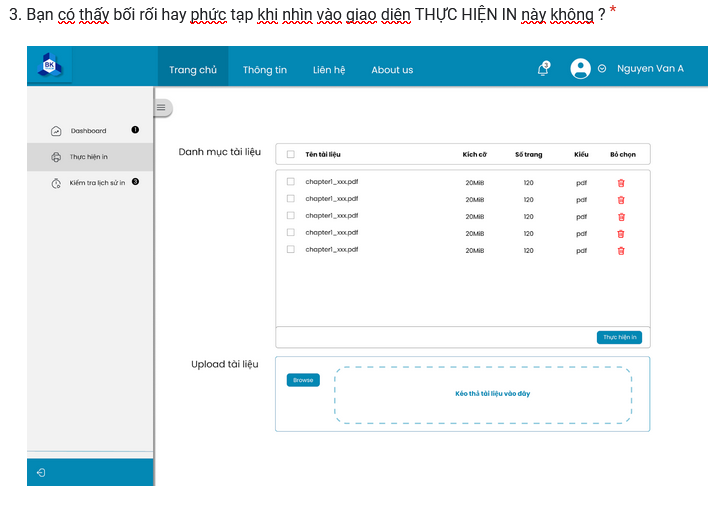
\includegraphics[width=0.8\linewidth]{images/image_uasbility/Q3_Stu.png}
    \caption{PRINTING PAGE}
    \label{fig:PRINTING PAGE}
\end{figure}
\newpage
According the survey, there are 40\% of participants find it a little curious to understand this task.
\begin{figure}[!h]
    \centering
    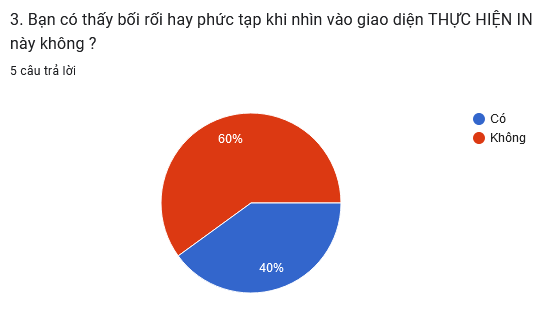
\includegraphics[width=0.8\linewidth]{images/image_uasbility/A3_Stu.png}
    \caption{Chart illustrates the result of Question 3}
    \label{fig:Chart illustrates the result of Question 3}
\end{figure}

    \item \textbf{PRINTING CONFIGURATION PAGE} \\
    In this Question, we research the behavior of participants in using PRINTING CONFIGURATION PAGE.
\begin{figure}[!h]
    \centering
    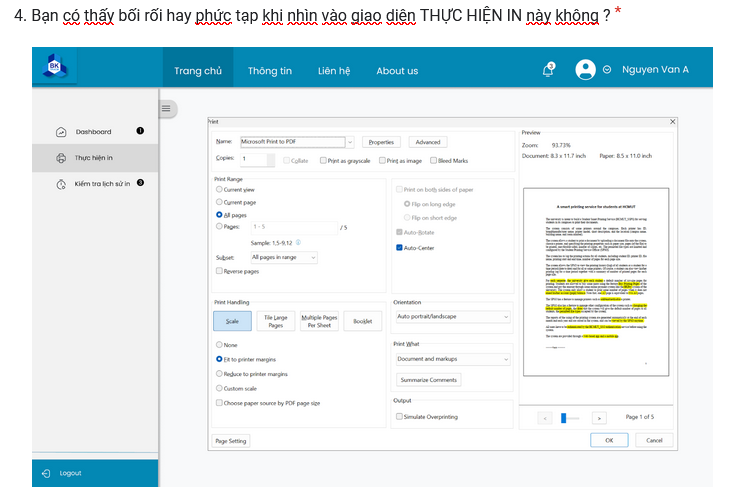
\includegraphics[width=0.8\linewidth]{images/image_uasbility/Q4_Stu.png}
    \caption{PRINTING CONFIGURATION PAGE}
    \label{fig:PRINTING CONFIGURATION PAGE}
\end{figure}
\newpage
According the survey, there are 40\% of participants find it a little curious to understand this task.
\begin{figure}[!h]
    \centering
    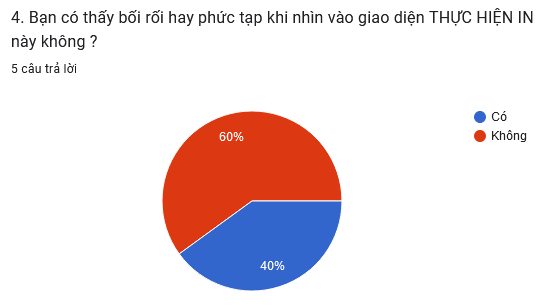
\includegraphics[width=0.8\linewidth]{images/image_uasbility/A4_Stu.png}
    \caption{Chart illustrates the result of Question 4}
    \label{fig:Chart illustrates the result of Question 4}
\end{figure}

    \item \textbf{HISTORY LOG PAGE} \\
    In this Question, we research the behavior of participants in using HISTORY LOG PAGE.
\begin{figure}[!h]
    \centering
    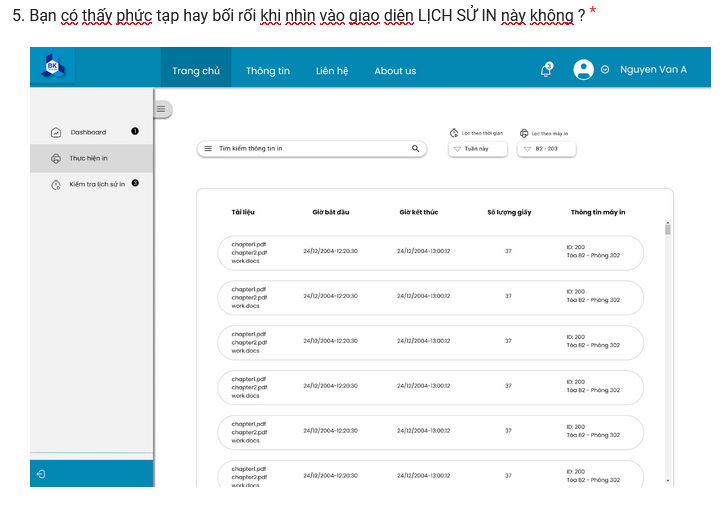
\includegraphics[width=0.8\linewidth]{images/image_uasbility/Q5_Stu.png}
    \caption{HISTORY LOG PAGE}
    \label{fig:HISTORY LOG PAGE}
\end{figure}
\newpage
According the survey, there are 40\% of participants find it a little curious to understand this task.
\begin{figure}[!h]
    \centering
    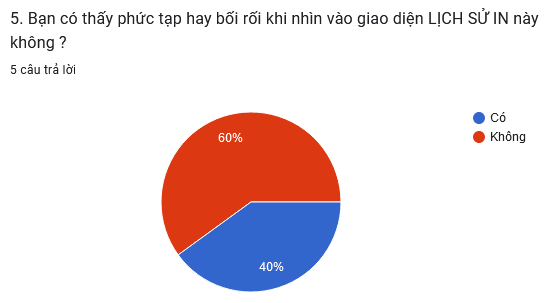
\includegraphics[width=0.8\linewidth]{images/image_uasbility/A5_Stu.png}
    \caption{Chart illustrates the result of Question 5}
    \label{fig:Chart illustrates the result of Question 5}
\end{figure}
\end{enumerate}

\subsection{SPSS for SPSO}
\begin{enumerate}
    \item \textbf{LOGIN PAGE} \\
    In this question, we research the behavior of participants in using LOGIN PAGE.
\begin{figure}[!h]
    \centering
    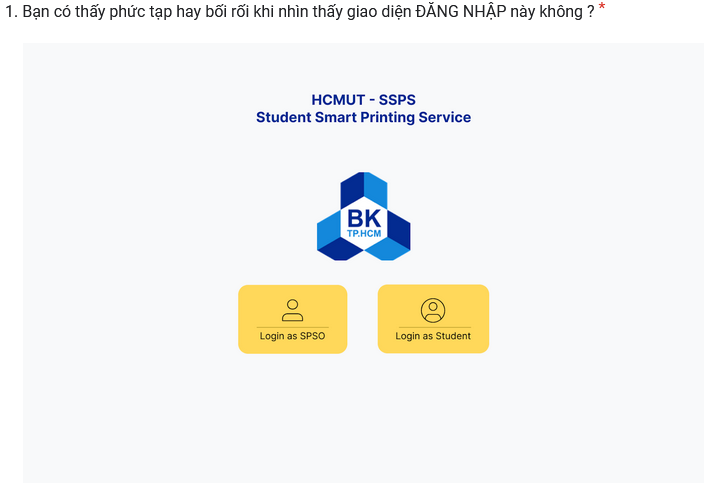
\includegraphics[width=0.8\linewidth]{images/image_uasbility/Q1_SPSO.png}
    \caption{LOGIN PAGE}
    \label{fig:LOGIN PAGE}
\end{figure}
\newpage
According to the survey, there are 60\% of participants find it a little curious to understand this task.
\begin{figure}[!h]
    \centering
    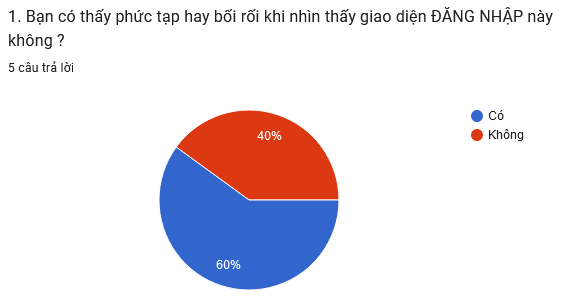
\includegraphics[width=0.8\linewidth]{images/image_uasbility/A1_SPSO.png}
    \caption{Char illustrates the result of Question 1}
    \label{fig:Chat illustrates the results of Question 1}
\end{figure}


    \item \textbf{DASHBOARD PAGE} \\
    In this Question, we research the behavior of participants in using DASHBOARD PAGE.
\begin{figure}[!h]
    \centering
    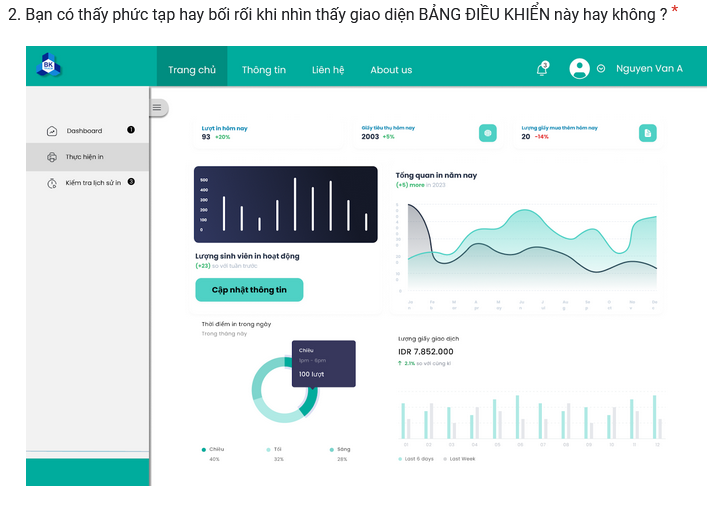
\includegraphics[width=0.8\linewidth]{images/image_uasbility/Q2_SPSO.png}
    \caption{DASHBOARD PAGE}
    \label{fig:DASHBOARD}
\end{figure}
\newpage
According to the survey, there are 60\% of participants find it a little curious to understand this task.
\begin{figure}[!h]
    \centering
    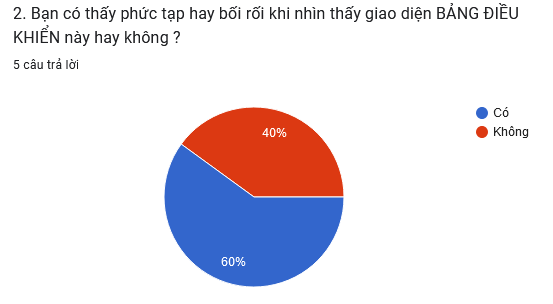
\includegraphics[width=0.8\linewidth]{images/image_uasbility/A2_SPSO.png}
    \caption{Chart illustrates the result of Question 2}
    \label{fig:Chart illustrates the result of Question 2}
\end{figure}


    \item \textbf{PRINTING CONFIGURATION PAGE} \\
    In this Question, we research the behavior of participants in using PRINTING CONFIGURATION PAGE.
\begin{figure}[!h]
    \centering
    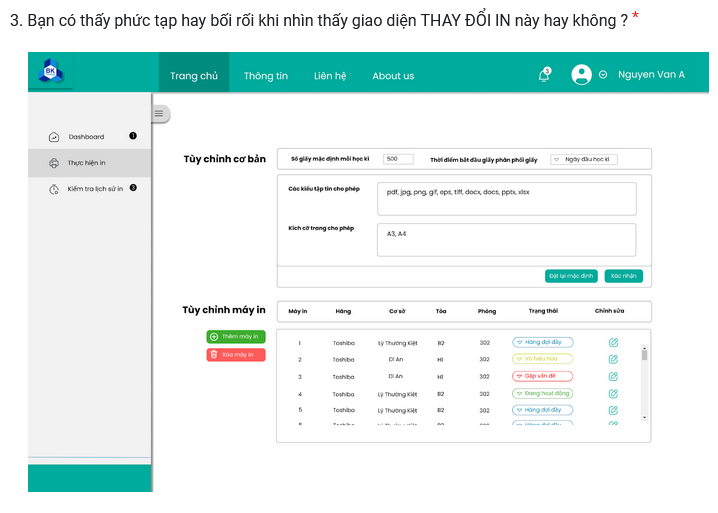
\includegraphics[width=0.8\linewidth]{images/image_uasbility/Q3_SPSO.png}
    \caption{PRINTING CONFIGURATION PAGE}
    \label{fig:PRINTING CONFIGURATION}
\end{figure}
\newpage
According the survey, there are 60\% of participants find it a little curious to understand this task.
\begin{figure}[!h]
    \centering
    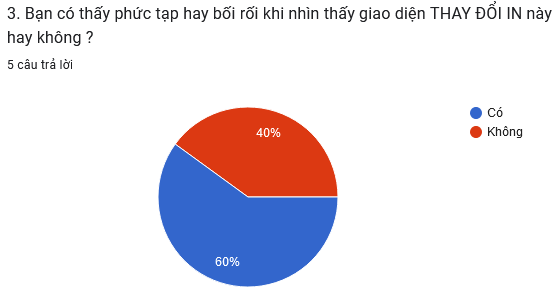
\includegraphics[width=0.8\linewidth]{images/image_uasbility/A3_SPSO.png}
    \caption{Chart illustrates the result of Question 3}
    \label{fig:Chart illustrates the result of Question 3}
\end{figure}


    \item \textbf{HISTORY LOG PAGE} \\
    In this Question, we research the behavior of participants in using HISTORY LOG PAGE.
\begin{figure}[!h]
    \centering
    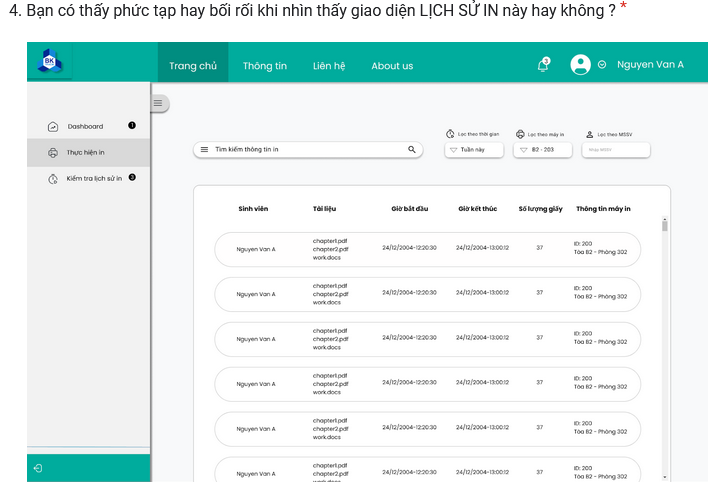
\includegraphics[width=0.8\linewidth]{images/image_uasbility/Q4_SPSO.png}
    \caption{HISTORY LOG PAGE}
    \label{fig:HISTORY LOG PAGE}
\end{figure}
\newpage
According the survey, there are 20\% of participants find it a little curious to understand this task.
\begin{figure}[!h]
    \centering
    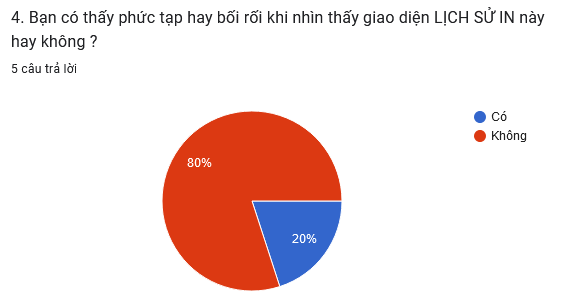
\includegraphics[width=0.8\linewidth]{images/image_uasbility/A4_SPSO.png}
    \caption{Chart illustrates the result of Question 4}
    \label{fig:Chart illustrates the result of Question 4}
\end{figure}
\end{enumerate}

\end{document}

